\chapter{The Hyperbolic Case: The Strata \texorpdfstring{$(3;1^6;3)$}{(3;1\textasciicircum 6;3)} and \texorpdfstring{$(2;1^6;3^2)$}{(2;1\textasciicircum 6;3\textasciicircum 2)} on the Disk}
\label{chap:stratatraintrackanalysis}

\section{Introduction}

In this chapter, we detail the classification of pseudo-Anosov 6-braids belonging to the strata $(3;1^6;3)$ and $(2;1^6;3^2)$ whose canonical lifts to the surface $\Sigma_2^2$ are fixed-point-free. These strata cannot be eliminated using the orientable foliations technique developed in Chapter \ref{chap:stratoriented} because their invariant train tracks contain odd-sided unmarked polygons (specifically 3-gons). Consequently, their invariant foliations are non-orientable, meaning we cannot apply the Alexander polynomial obstruction directly to the geometric data. Instead, we must explicitly enumerate and analyze the specific train track maps carried by the allowable standard train tracks in these strata.

Our analysis proceeds in several steps. First, the finite list of candidate standard train tracks is generated by the \texttt{autofolder} algorithm, and among these we retain the ones which are jointless. By utilizing the tight splitting sequences established in Chapter \ref{chap:tight_splitting}, we further reduce the number of tracks that need to be considered. We further reduce the number by identifying train tracks that are vertical mirror images of each other; since the mirror of a braid inducing a map on one track induces a symmetric map on the other, it suffices to analyze a single representative from each mirror pair.

For the stratum $(3;1^6;3)$, this reduction process isolates a single standard jointless train track, which we refer to as \textit{The Candelabra} (see Figure \ref{fig:candelabra}). For the stratum $(2;1^6;3^2)$, the tight splitting sequences reduce the candidate list to exactly six tracks. Therefore, up to conjugation, mirroring, and the addition of full twists, every fixed-point-free pseudo-Anosov 6-braid in these two strata must be carried by one of these specific train tracks.

We then exhaustively analyze all possible train track maps that can be carried by each of these refined tracks. The analysis proceeds edge by edge, enumerating the admissible image paths $f_\beta(e)$ subject to two combinatorial obstructions: the Trace Lemma (which forbids self-occurrence at jointless monogon edges and imposes parity constraints at the central edge $d$ of two-triangle tracks) and the Absorption Obstruction (which forbids image paths from entering geometrically inaccessible regions near vertices). When neither obstruction can be satisfied, the configuration falls into one of three named patterns---Situation $\alpha$, Situation $\beta$, or a path mill---each of which produces a contradiction; we collect these in Appendix \ref{app:case_analysis_preliminaries}. This procedure successfully prunes the infinite space of maps down to a finite list of eligible train track map \textit{families} for each track. For each surviving family, we produce explicit braid words $\beta$ that induce those maps.

Finally, to verify if such a braid $\beta$ can properly fit into the Birman-Hilden correspondence data
\[
(h, \phi_h, \hat{h}, \hat{\phi}_h, b, \phi_b, \beta, \phi_\beta, \Phi, \phi_\Phi)
\]
induced by the monodromy $h$ of a hyperbolic fibered knot $K$ satisfying $\widehat{HFK}(K) \cong \widehat{HFK}(T_{2,3}\# T_{2,3})$, we apply two homological filters. We compute the action of the open book decomposition induced by $\beta$ on the first homology to ensure it bounds the correct ambient manifold, and we extract its Alexander polynomial. We demonstrate that none of the candidate braid families generated by the train track analysis satisfy these necessary homological conditions, allowing us to definitively rule out both strata.


\section{Topological Constraints on Train Track Maps}
\label{sec:traintrack_analysis}

Fixing a stratum of pseudo-Anosov maps on the 6-marked disk (either $(3;1^6;3)$ or $(2;1^6;3^2)$), the \texttt{autofolder} algorithm produces a finite list of standard train tracks. Among these, we restrict our attention solely to the jointless standard train tracks, as any pseudo-Anosov map in this stratum is guaranteed to be carried by one such track (Corollary \ref{cor:jointless_track}).

Let $\tau$ be one such jointless standard train track. We aim to enumerate all possible train track maps $f_\beta$ carried by $\tau$, subject to the strict topological condition that any 6-braid $\beta$ inducing $f_\beta$ must lift to a fixed-point-free pseudo-Anosov map on the genus-two surface $\Sigma_2^2$. This topological condition places severe combinatorial constraints on the underlying train track map on the disk.

\subsection{The Trace Lemma}

The relationship between the transition matrix of a train track map on the disk and the fixed-point theory of its lift is encapsulated by the Trace Lemma, which was first established as Lemma \ref{lem:trace_lemma} in Chapter \ref{chap:train tracks}. We restate it below in the form most useful for our case analysis, after introducing the necessary local terminology.

Recall that a standard train track on the marked disk possesses a unique edge belonging to the infinitesimal polygon incident to each marked point. We refer to these as \textbf{side-swapping edges}. The geometric significance of such an edge is that because the double cover is branched exactly over the marked points, whenever a train path on the disk traverses a side-swapping edge, its canonical lift to the surface strictly transitions to the ``other sheet'' of the cover.

We adapt the following lemma and corollary from Reinoso \cite[Chapter~2]{reinoso2024pseudo} to our setting.

\begin{lemma}[The Trace Lemma]\label{lem:trace_lemma_downstairs}
Let $(\beta, \phi_\beta, \tau, f_\beta)$ be the geometric data of a pseudo-Anosov braid with Birman-Hilden lift $(h, \phi_h, \tilde{\tau}, \tilde{f}_h)$ on the surface $\Sigma_2^2$. Suppose that $\tau$ is a standard train track and that the canonical lift $\phi_h$ has no interior fixed points on $\Sigma_2^2$. Then, for any real edge $e$ of $\tau$, any sub-word of the image path $f_\beta(e)$ bounded by two occurrences of $e$ must contain an \textbf{even} number of side-swapping edges.
\end{lemma}

\begin{proof}
If the canonical lift $\phi_h$ has no interior fixed points, its transition matrix $M(\tilde{f}_h)$ must be strictly traceless by \cite[Proposition~2.2.4]{reinoso2024pseudo}. Consequently, for any real edge $e_i$ in the lifted track $\tilde{\tau}$, the edge $e_i$ cannot appear in its own image $\tilde{f}_h(e_i)$.

Consider the image path $f_\beta(e)$ on the disk. Every traversal of a side-swapping edge causes the image $\tilde{f}_h(e_i)$ of either lift of $e$ to cross to the opposite sheet of the branched cover. If $e$ appeared in $f_\beta(e)$ separated by an odd number of side-swapping edges, then the lifted image $\tilde{f}_h(e_1)$ would necessarily map back onto $e_1$ (and similarly for $e_2$). This would force a non-zero diagonal entry of $M(\tilde{f}_h)$, contradicting the tracelessness established above.
\end{proof}

In our context, the standard train tracks generated for these strata feature jointless monogons at the marked points. This specific local geometry allows for a highly restrictive corollary.

\begin{corollary}[Trace Lemma for Jointless Monogons]\label{cor:trace_jointless}
Retain the notation and assumptions of Lemma \ref{lem:trace_lemma_downstairs}. If $e$ is a real edge of $\tau$ which is directly incident to a jointless monogon at a marked point, then $e$ cannot appear anywhere in its own image path $f_\beta(e)$.
\end{corollary}

\begin{proof}
Suppose, for the sake of contradiction, that $e$ appears in $f_\beta(e)$. Because $e$ is incident to a jointless monogon (which has only one real edge attached to it), any path entering the monogon via $e$ must immediately exit via $e$, effectively ``turning around''. This forces two adjacent, consecutive appearances of $e$ in the word $f_\beta(e)$. Since there are zero side-swapping edges between these two occurrences, it violates the parity condition of Lemma \ref{lem:trace_lemma_downstairs}.

Alternatively, if the path $f_\beta(e)$ terminates entirely upon reaching $e$, it implies that the vertex corresponding to the monogon is mapped to itself. This local invariance generates an interior fixed point at the singularity in the lifted surface, which again contradicts the assumption that $\phi_h$ is fixed-point-free. Thus, $e$ cannot appear in $f_\beta(e)$.
\end{proof}

In the stratum $(3;1^6;3)$, all of the real edges of the train tracks under consideration are incident to a jointless monogon, thus Corollary \ref{cor:trace_jointless} applies. In the stratum $(2;1^6;3^2)$, all but a single real edge $d$ connecting the two unmarked triangles are incident to a jointless monogon. Thus Corollary \ref{cor:trace_jointless} applies to all real edges except $d$. Consequently, in our enumeration of possible train track maps, the image path of real edges except $d$ cannot contain itself.

\subsection{The Absorption Obstruction}
\label{subsec:absorption_obstruction}

While the Trace Lemma places strict algebraic restrictions on the transition words, we must also ensure the geometric validity of the map $f_\beta$. Because $f_\beta$ is induced by a genuine, injective surface homeomorphism $\phi_\beta$, it must preserve the injectivity of train paths. This requirement imposes local geometric rigidity near the vertices of $\tau$, formalized through the concept of \textit{absorption}.

\begin{definition}
Let $a$ and $b$ be two real edges of $\tau$ adjacent at an initial vertex $v$. The initial segments of the mapped edges $\phi_\beta(a)$ and $\phi_\beta(b)$ determine a convex cone extending from $\phi_\beta(v)$, denoted $X_v(a,b)$, lying transverse to the invariant foliations of the surface.
\end{definition}

\begin{lemma}[The Absorption Obstruction, {\cite[Lemma~4.2.5]{reinoso2024pseudo}}]
\label{lem:cone_condition}
For any real edge $c$ of $\tau$, the image path $\phi_\beta(c)$ cannot intersect the interior of the convex cone $X_v(a,b)$.
\end{lemma}

\begin{proof}
By the injectivity of the diffeomorphism $\phi_\beta$, the path $\phi_\beta(c)$ cannot cross the boundary of the cone, which is formed strictly by the paths $\phi_\beta(a)$ and $\phi_\beta(b)$. Suppose, for the sake of contradiction, that $\phi_\beta(c)$ enters the interior of $X_v(a,b)$.

Since $\phi_\beta(c)$ cannot cross the boundary to exit, it must either terminate strictly inside the cone, or exit by backtracking through the vertex $\phi_\beta(v)$. Backtracking is impossible for a taut train track map. Furthermore, the endpoints of real edges in a standard train track map only to marked points or singularities, which are permuted by $\phi_\beta$. The local structure at $\phi_\beta(v)$ prescribes a strict cyclic ordering of the incident edges. If $c$ is distinct from $a$ and $b$, its image cannot essentially land ``between'' $\phi_\beta(a)$ and $\phi_\beta(b)$ without violating the preservation of this cyclic order or destroying the planar embedding of the graph. Thus, $\phi_\beta(c)$ cannot enter the cone $X_v(a,b)$.
\end{proof}

\begin{figure}[ht]
    \centering
    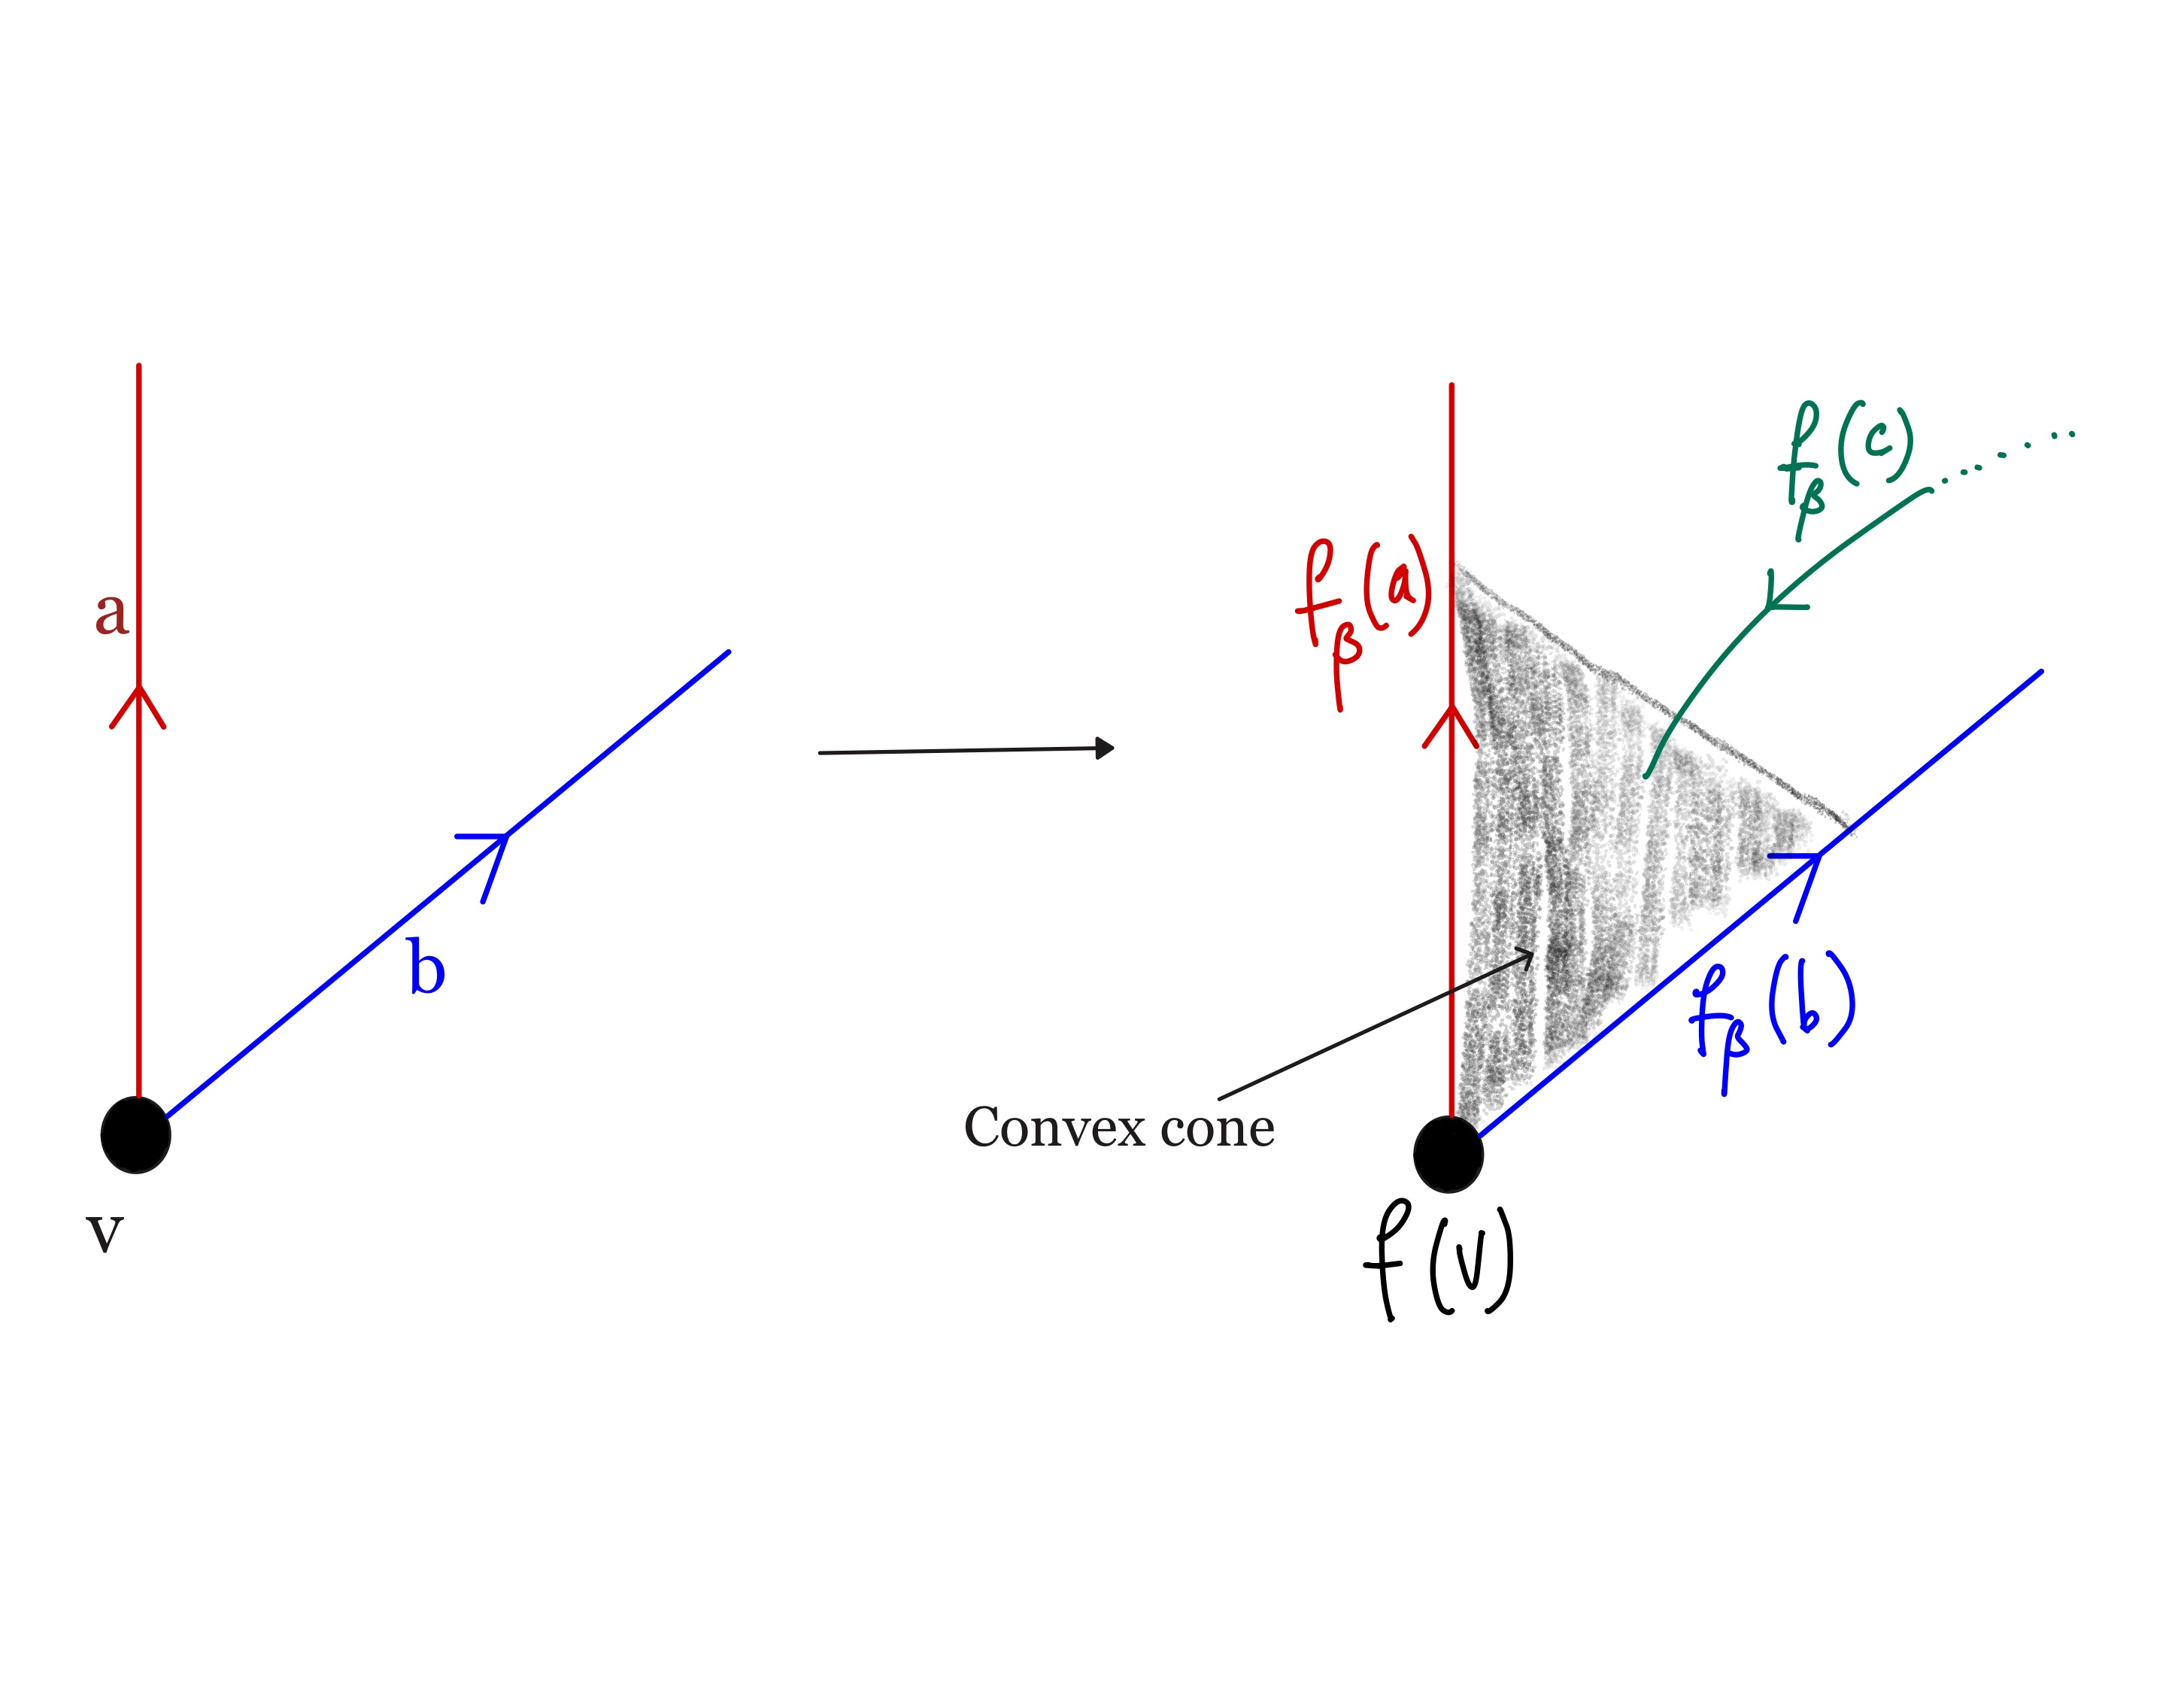
\includegraphics[width=0.8\linewidth]{figures/Absorption-1.jpg}
    \caption[The Absorption Obstruction]{An invalid geometric configuration where $\phi_\beta(c)$ is absorbed between $\phi_\beta(a)$ and $\phi_\beta(b)$, violating injectivity.}
    \label{fig:absorbed_cone}
\end{figure}

When the theoretical transition word $f_\beta(c)$ implies that the path $\phi_\beta(c)$ enters $X_v(a,b)$, we say that $f_\beta(c)$ is \textbf{absorbed} between $f_\beta(a)$ and $f_\beta(b)$ (illustrated in Figure \ref{fig:absorbed_cone}). We denote such a disallowed scenario in our hypothetical image paths with an $\times$ superscript:
\[
f_\beta(c) = \dots \Abso{f_\beta(a)}{f_\beta(b)} \dots
\]
The existence of such an absorption immediately invalidates the transition word. By systematically applying the Absorption Obstruction alongside the algebraic parity constraints of the Trace Lemma, we can definitively prune the space of possible transition matrices.



\subsection{The Case Analysis Procedure}
\label{subsec:case_analysis_procedure}

Given a jointless standard train track $\tau$, we enumerate the families of train track maps $f_\beta$ carried by $\tau$ via the following procedure. Steps 1--6 below constitute the content of the per-track case analyses in Appendices \ref{app:case_analysis_candelabra}, \ref{app:case_analysis_track0}, \ref{app:case_analysis_track1}, \ref{app:case_analysis_track8}, \ref{app:case_analysis_track12}, \ref{app:case_analysis_track13}, and \ref{app:case_analysis_track17}; Step 7 is the content of the corresponding braid-extraction appendices.

\begin{enumerate}
    \item \textbf{Initial labeling.} Label and orient the real edges of $\tau$ toward their adjacent monogons. For two-triangle tracks, identify the central edge $d$ connecting the two infinitesimal triangles and its symmetric companion $\bar{d}$.
    
    \item \textbf{Triangle permutation case split.} For two-triangle tracks, branch the analysis into Cases A, B, C, D according to how $f_\beta$ permutes the two infinitesimal triangles, as described in Section \ref{subsec:path_notation_two_triangles}.
    
    \item \textbf{Initial-letter enumeration.} For each real edge $e$ of $\tau$, enumerate the possible first letters of $f_\beta(e)$, subject to Corollary \ref{cor:trace_jointless} (the letter $e$ does not appear in $f_\beta(e)$) and, in Case A, the parity constraint of Assumption A applied to $f_\beta(d)$ and $f_\beta(\bar{d})$.
    
    \item \textbf{Forced continuations.} For each partial image path, determine the next admissible letters by checking the Trace Lemma (for paths at the central edge $d$, the parity of the number of letters between consecutive $d$-crossings) and the Absorption Obstruction (at each vertex traversed, the image path must not enter a cone formed by adjacent edge images, as in Lemma \ref{lem:cone_condition}).
    
    \item \textbf{Termination or contradiction.} Continue Step 4 until either (i) the path terminates with a $\circ$-decoration at a marked point, yielding a candidate, or (ii) the path is forced into Situation $\alpha$, Situation $\beta$, a path mill, or a direct tracing or absorption violation, eliminating the case. See Appendix \ref{app:case_analysis_preliminaries} for the precise definitions of Situations $\alpha$, $\beta$, and path mills, together with worked examples of each contradiction pattern.
    
    \item \textbf{Parameterization.} Group surviving paths into families parameterized by the number of internal twists $k$ between adjacent edges, accommodating the fact that an edge image may twist between two adjacent edges an arbitrary number of times before terminating.
    
    \item \textbf{Braid extraction.} For each surviving family, reverse-engineer a braid word $\beta$ inducing the family by isotoping the image train track back to $\tau$. This is illustrated explicitly for the candelabra example below and for the Jehu family in Appendix \ref{app:candidate_braids_candelabra}.
\end{enumerate}

We now demonstrate this procedure with two worked examples: first on the candelabra (one infinitesimal triangle, no central edge $d$), then on Track 0 (two infinitesimal triangles, with the central edge analysis in full).

\subsection{Path Notation and The Two Triangles}
\label{subsec:path_notation_two_triangles}

Following the conventions established by Reinoso \cite{reinoso2024pseudo}, we describe the image of a real edge under the train track map $f_\beta$ as a sequence of real edges decorated with turn information. Let $\tau$ be a standard train track. The image path $f_\beta(e)$ is represented as a word in the real edges $\{x_1, \dots, x_k\}$ of $\tau$.


Each letter is equipped with a decoration from $\{+, -, \circ\}$ indicating the behavior of the path at the vertex reached after traversing that edge:
\begin{itemize}
    \item $x^+$ indicates the path traverses edge $x$ and turns in the \textbf{positive} direction (typically left relative to the orientation) at the vertex to enter the next edge.
    \item $x^-$ indicates the path traverses edge $x$ and turns in the \textbf{clockwise} direction to enter the next edge.
    \item $x^\circ$ indicates the path traverses edge $x$ and \textbf{terminates} at the marked point inside the associated polygon. This decoration appears only on the final edge of the path.
\end{itemize}

As noted previously, the invariant train tracks carrying our candidate pseudo-Anosov braids fall into two distinct geometric categories based on their central singularities. The single track in stratum $(3;1^6;3)$ (\textit{The Candelabra}) possesses only one infinitesimal triangle, while the five candidate tracks in $(2;1^6;3^2)$ feature a central edge $d$ connecting exactly \textbf{two} infinitesimal triangles.

For the two-triangle tracks, the constraints on the image $f_\beta(d)$ are governed entirely by how $f_\beta$ permutes these triangles downstairs, and how $\tilde{f}_h$ permutes their canonical lifts upstairs. Because the surface $\Sigma_2^2$ is a double cover branched over the marked points, we can partition the admissible behavior of $f_\beta$ into four exhaustive cases based on the permutation of the pre-images of the triangles $\{p_1, p_2, p_3, p_4\}$ under the fixed-point-free map $\phi_h$:

\begin{itemize}
    \item \textbf{Case A (Triangles Fixed):} The infinitesimal triangles are fixed by $f_\beta$ downstairs. Under the lift, this occurs if and only if the lifts are swapped (sent to the opposite side of $\tilde{\tau}$) by $\tilde{f}_h$. \\
    \textbf{Trace Constraint:} For $\tilde{f}_h$ to prevent the lifted edge $\tilde{d}$ from mapping over itself on the same sheet, every occurrence of $d$ or $\overline{d}$ in $f_\beta(d)$ must occur after an \textbf{even} number of preceding letters.

    \item \textbf{Case B (Triangles Swapped - Both Same Side):} The triangles are swapped downstairs, and both of their lifts are sent to the same side of $\tilde{\tau}$. \\
    \textbf{Trace Constraint:} Because the boundary points of $d$ are exchanged, the path must switch its sheet parity to avoid an interior fixed point on $\tilde{d}$. Thus, at least one of $f_\beta(d)$ or $f_\beta(\overline{d})$ must pass over $d$ or $\overline{d}$ after an \textbf{odd} number of letters.

    \item \textbf{Case C \& D (Triangles Swapped - Mixed Sides):} The triangles are swapped downstairs; one lift is sent to the same side, and the other to the opposite side. \\
    \textbf{Trace Constraint:} Subject to the exact same \textbf{odd} parity constraint as Case B.
\end{itemize}

By systematically checking every theoretical transition word against these parity constraints and the Absorption Obstruction, we can computationally exhaust the finite set of valid train track maps for both strata.


\subsubsection*{Example 1: The Candelabra}
\label{subsec:example_candelabra}

We illustrate the procedure on the candelabra (Figure \ref{fig:candelabra}), the unique jointless standard train track in the stratum $(3;1^6;3)$ (as will be established in Section \ref{sec:analysis_3_16_3}). The candelabra has six real edges $b, o, s, i, p, r$, each incident to a jointless monogon, and a single central infinitesimal triangle. Because there is no central edge $d$, Step 2 of the procedure (the triangle permutation case split) does not arise here.

\paragraph{Step 1 (Initial labeling).} We label and orient the six real edges toward their respective monogons, as shown in Figure \ref{fig:candelabra}.

\paragraph{Step 3 (Initial letters).} By Corollary \ref{cor:trace_jointless}, the letter $e$ cannot appear in $f_\beta(e)$ for any of the six edges. This already constrains the first letter of each image path: for instance, $\fbb$ cannot begin with $b$, so it must begin with one of $o, s, i, p, r$ (with an appropriate decoration). Combined with the local cyclic order at each vertex, this immediately implies that the triangle must be rotated by $f_\beta$; otherwise at least one of $\fbb$ or $\fbr$ would immediately trace. Thus the complete case analysis must consider separately the case in which $\fbr$ and $\fbb$ begin with the pair $\{o^{*}, s^{*}\}$ in some order, and the case in which they begin with $\{i^{*}, p^{*}\}$ in some order. For the purpose of this example, we treat the former case. In this situation, $\fbo$ and $\fbs$ begin with the pair $\{i^{*}, p^{*}\}$ in some order, while $\fbi$ and $\fbp$ begin with the pair $\{b^{*}, r^{*}\}$ in some order. The complete case analysis enumerates all such possibilities; here we restrict to the following subcase:
\[
\fbp = b^\circ, \qquad \fbi = r^\circ,
\]
\[
\fbr = o^*\ldots, \qquad \fbb = o^*\ldots,
\]
\[
\fbo = p^*\ldots, \qquad \fbs = p^*\ldots.
\]
This initial state is shown in Figure \ref{fig:Jehu_example_1}.

\begin{figure}[H]
    \centering
    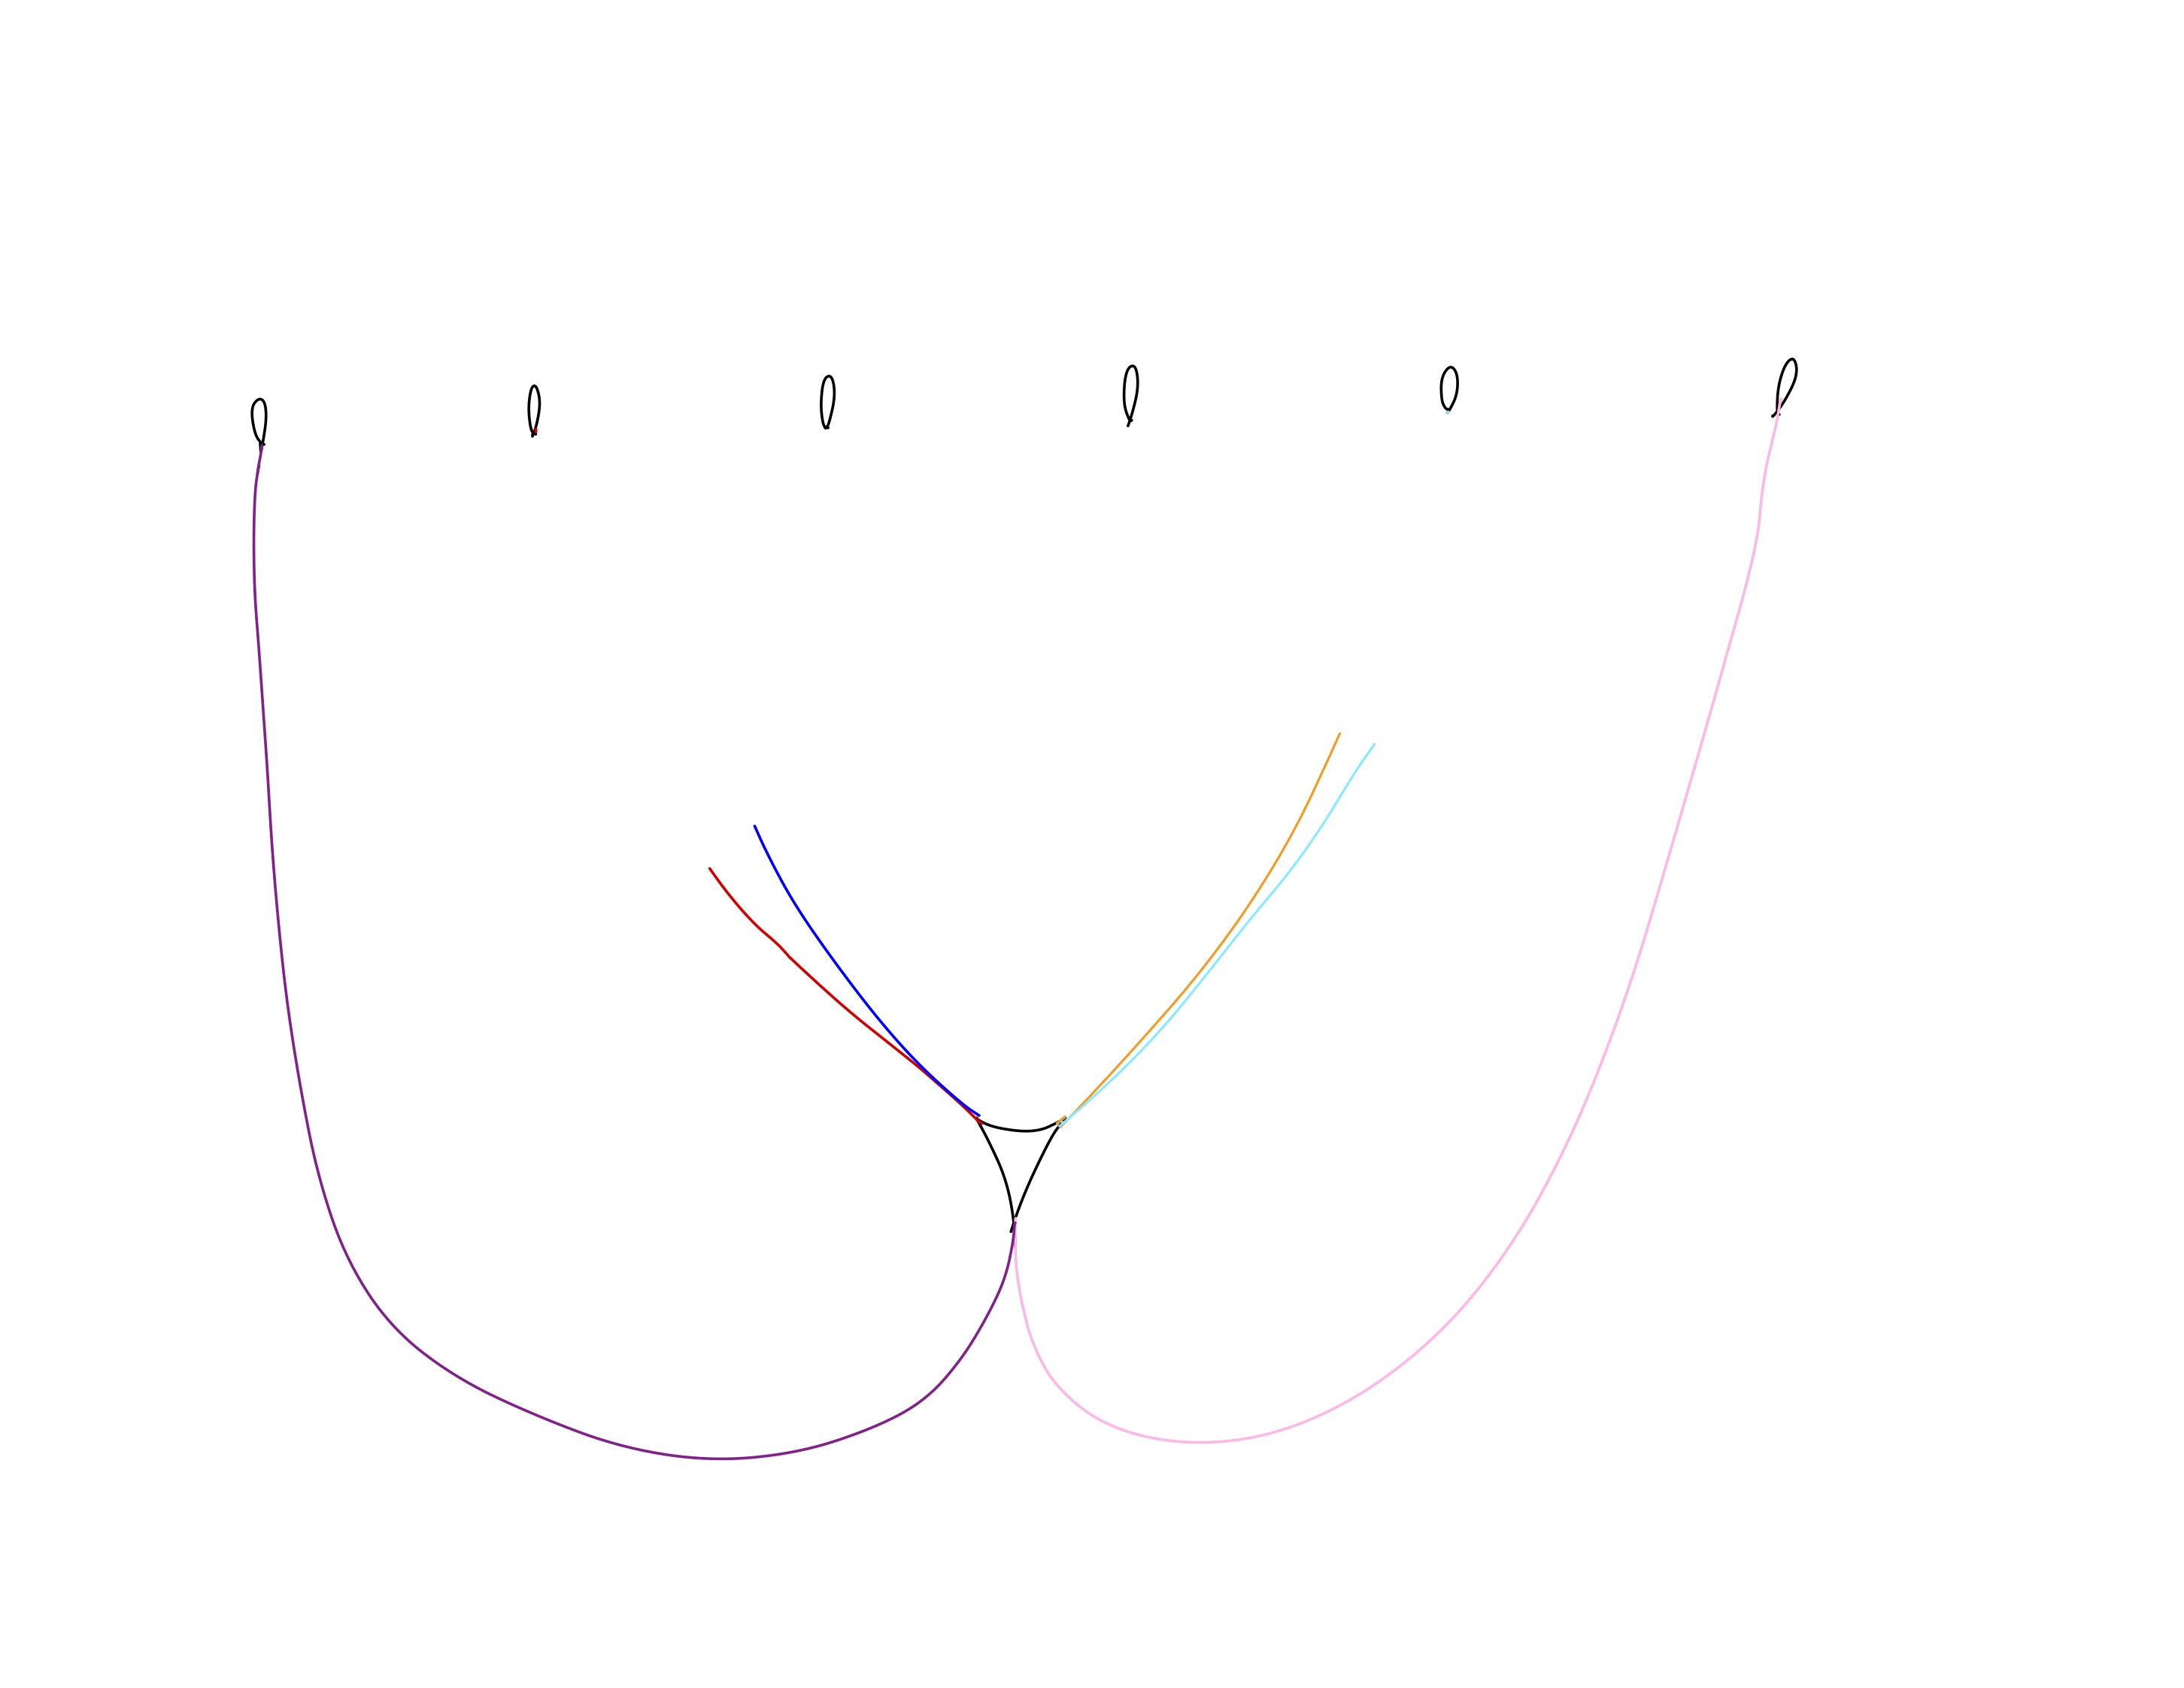
\includegraphics[width=\linewidth]{figures/Case Analysis Example Candelabra-01.jpg}
    \caption{Initial subcase under consideration: $\fbp = b^\circ$, $\fbi = r^\circ$, with $\fbr$ and $\fbb$ both beginning at $o$, and $\fbo$ and $\fbs$ both beginning at $p$.}
    \label{fig:Jehu_example_1}
\end{figure}

\paragraph{Step 4 (Forced continuations and absorption).} Within this subcase, the case analysis further branches on the decoration of each first letter. Let us first consider $\fbr$. If it were to begin with $o^\circ$ (meaning it terminates immediately) or $o^+$ (a counterclockwise turn), then because $\fbb$ lies to the right of $\fbr$, $\fbb$ would in both cases be forced to begin with $o^+$, and would then immediately trace:
\[
\fbb = o^+ b^\times,
\]
as shown in Figures \ref{fig:Jehu_example_2} and \ref{fig:Jehu_example_3}.

\begin{figure}[H]
    \centering
    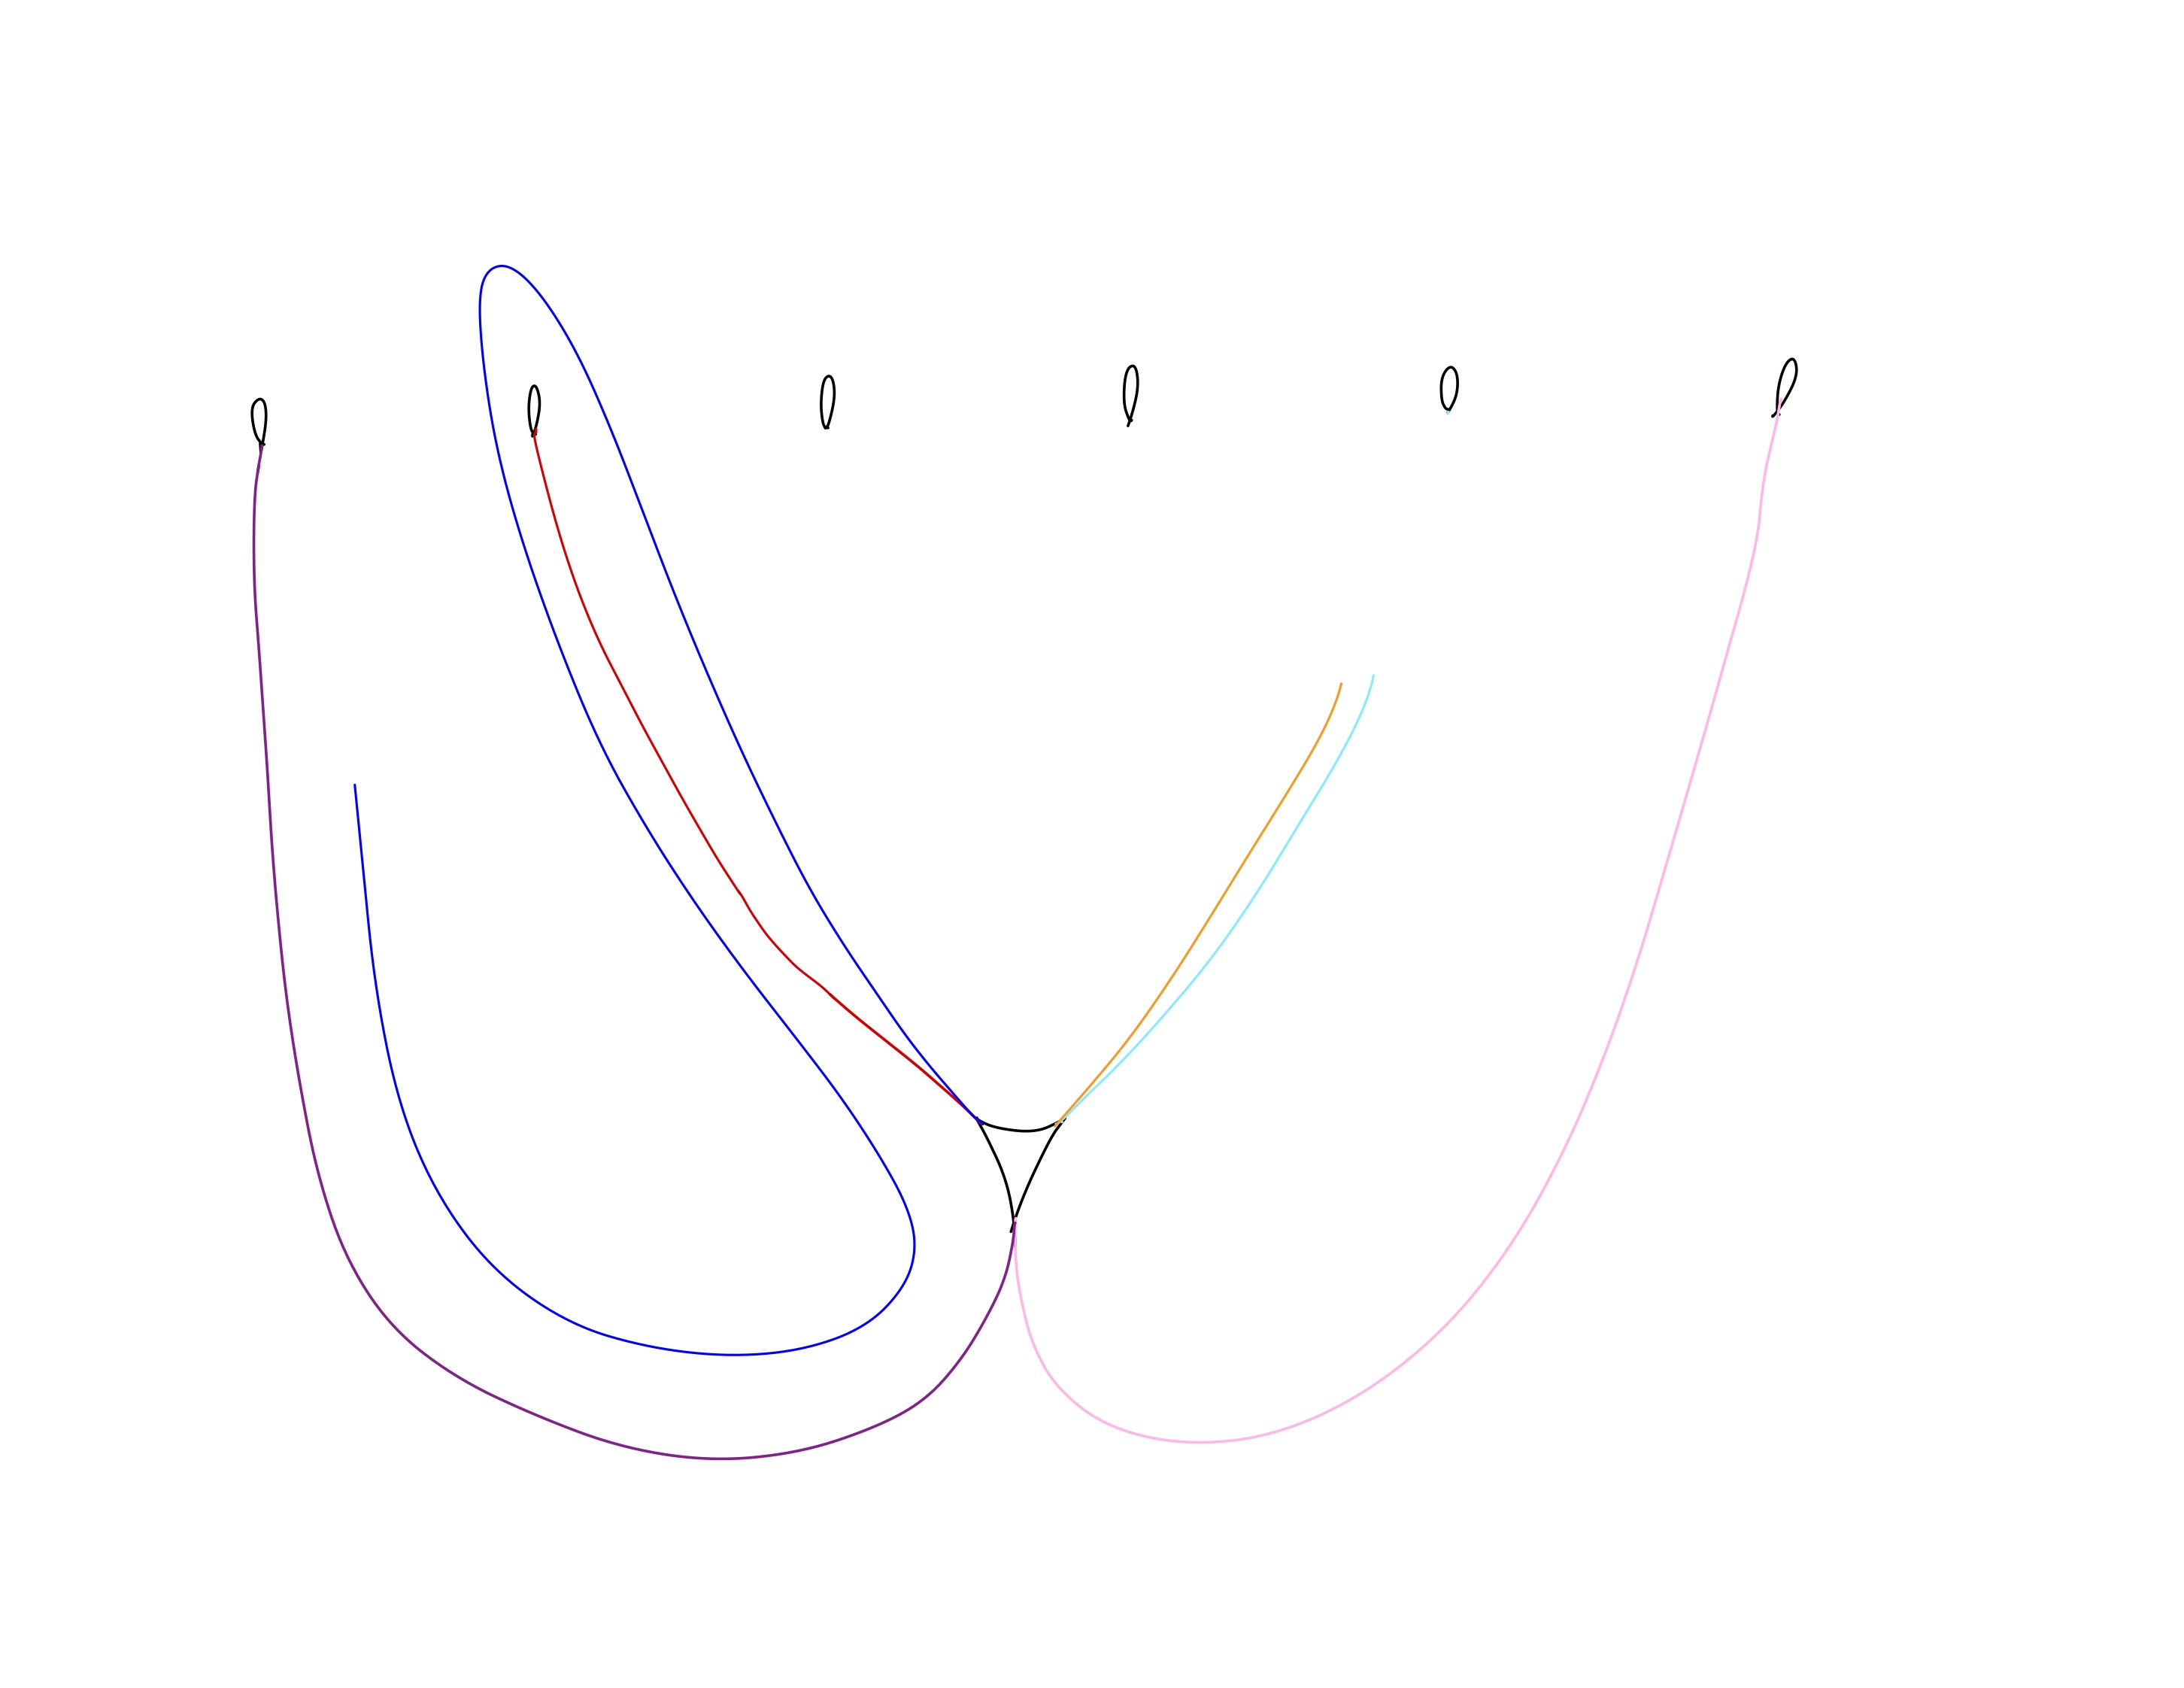
\includegraphics[width=\linewidth]{figures/Case Analysis Example Candelabra-02.jpg}
    \caption{Failure of the $\fbr = o^\circ$ branch: $\fbb$ is forced to begin with $o^+$ and traces immediately at $b^\times$.}
    \label{fig:Jehu_example_2}
\end{figure}

\begin{figure}[H]
    \centering
    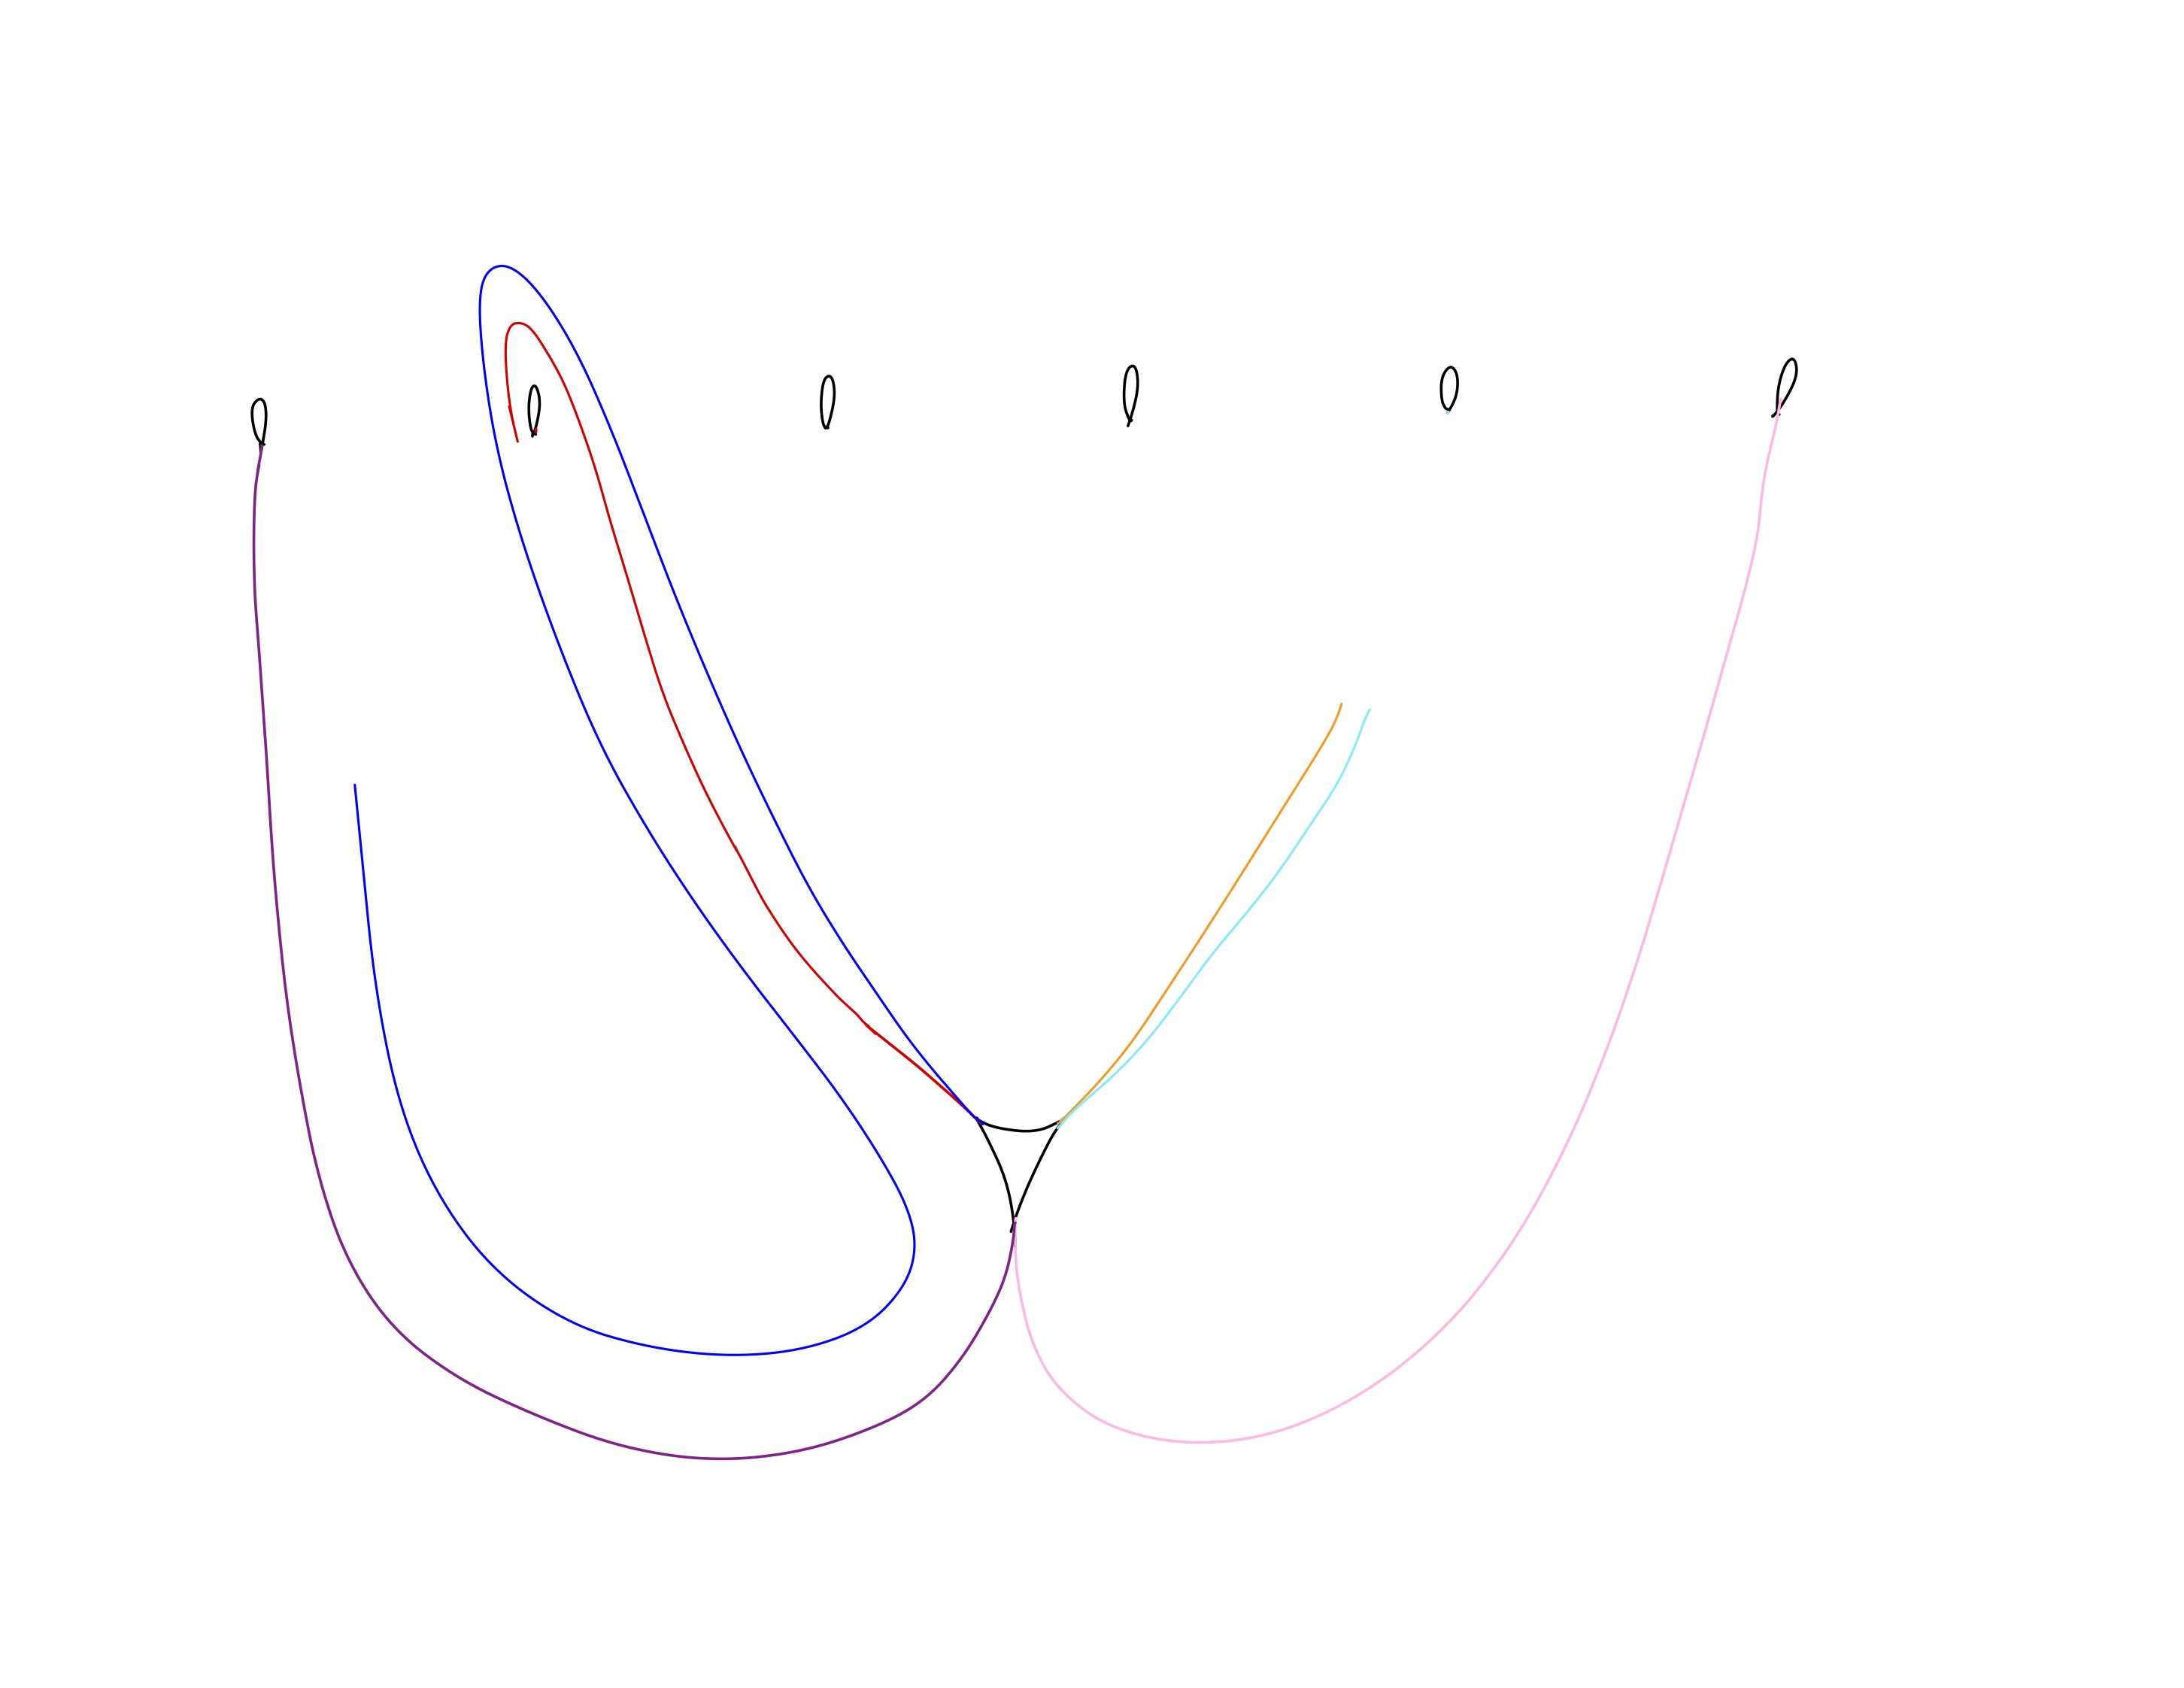
\includegraphics[width=\linewidth]{figures/Case Analysis Example Candelabra-03.jpg}
    \caption{Failure of the $\fbr = o^+$ branch: $\fbb$ is again forced into $o^+ b^\times$, tracing immediately.}
    \label{fig:Jehu_example_3}
\end{figure}

The only remaining possibility is for $\fbr$ to begin with $o^-$, entering to the right of $\fbb$ after the clockwise turn:
\[
\fbr = o^-\ldots,
\]
as shown in Figure \ref{fig:Jehu_example_4}. The next letter can then be either $i^{*}$ or $p^{*}$.

\begin{figure}[H]
    \centering
    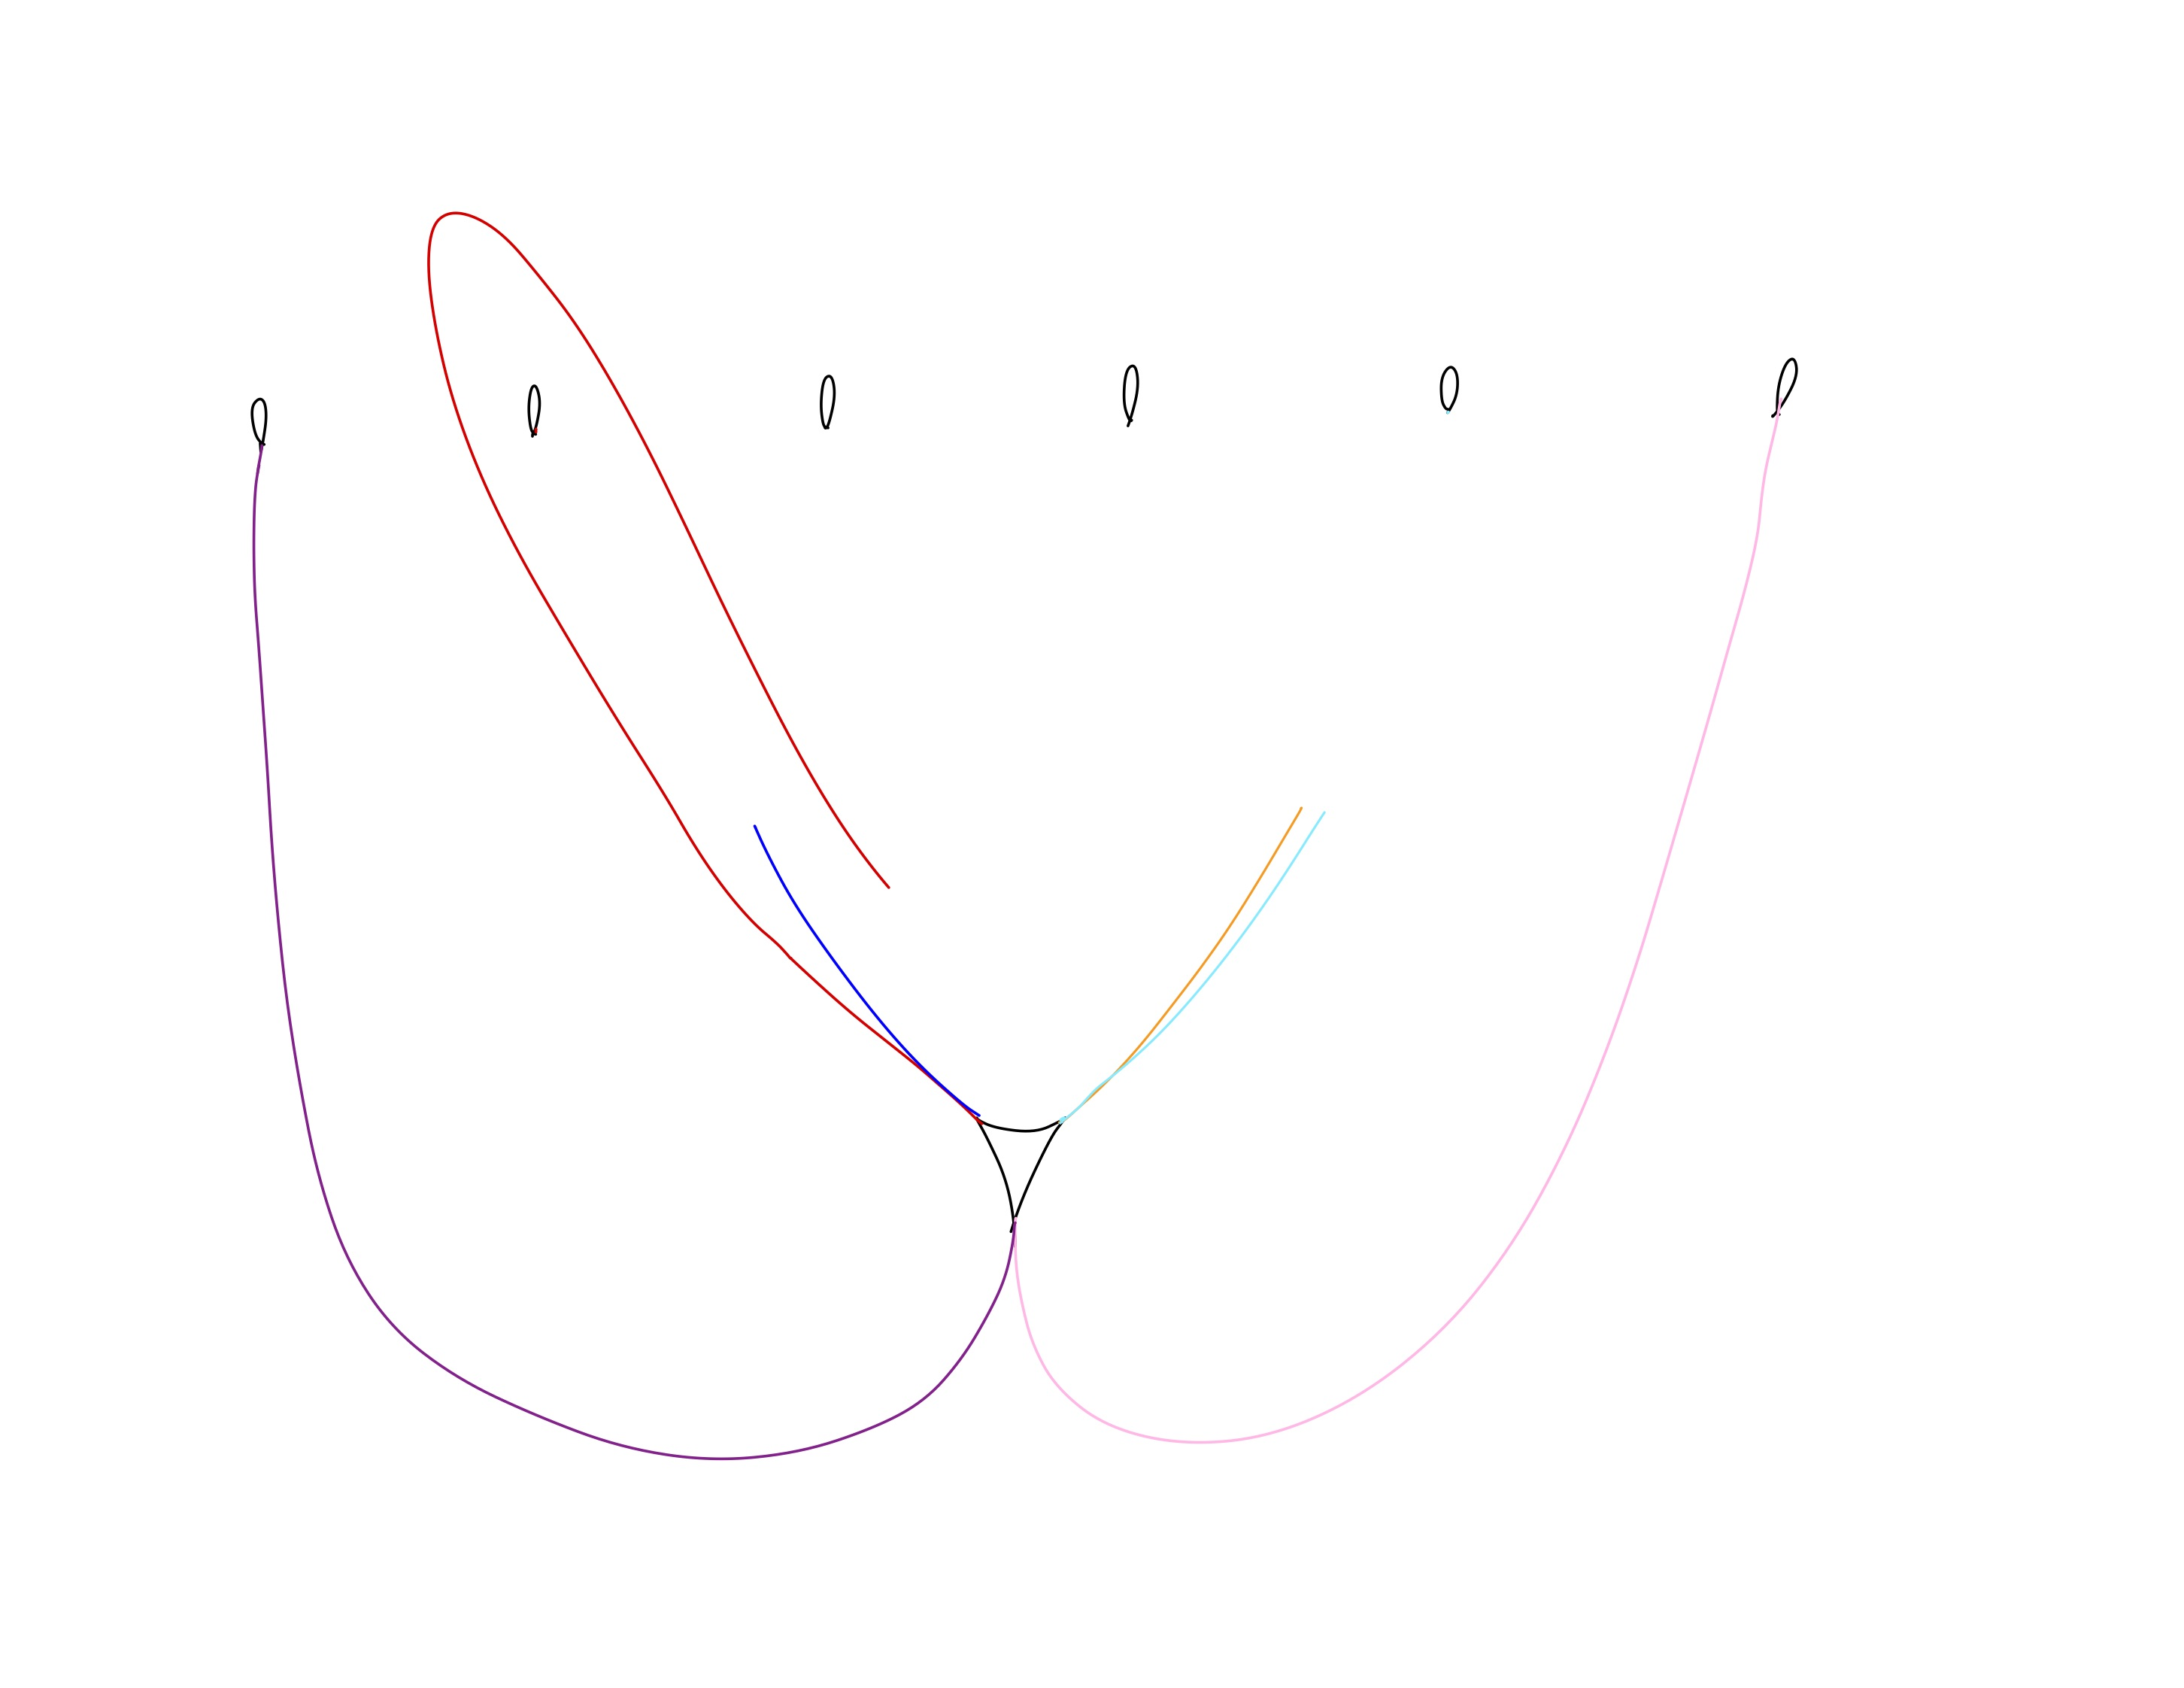
\includegraphics[width=\linewidth]{figures/Case Analysis Example Candelabra-04.jpg}
    \caption{The only admissible decoration: $\fbr = o^-\ldots$, with $\fbr$ entering to the right of $\fbb$ after the clockwise turn.}
    \label{fig:Jehu_example_4}
\end{figure}

Let us now turn to $\fbs$. If it were to begin with $p^\circ$ or $p^-$, then because $\fbo$ lies to the left of $\fbs$, $\fbo$ would be forced to begin with $p^-$ and would be absorbed:
\[
\fbo = p^- r^- \Abso{\fbp}{\fbi},
\]
as shown in Figure \ref{fig:Jehu_example_5}.

\begin{figure}[H]
    \centering
    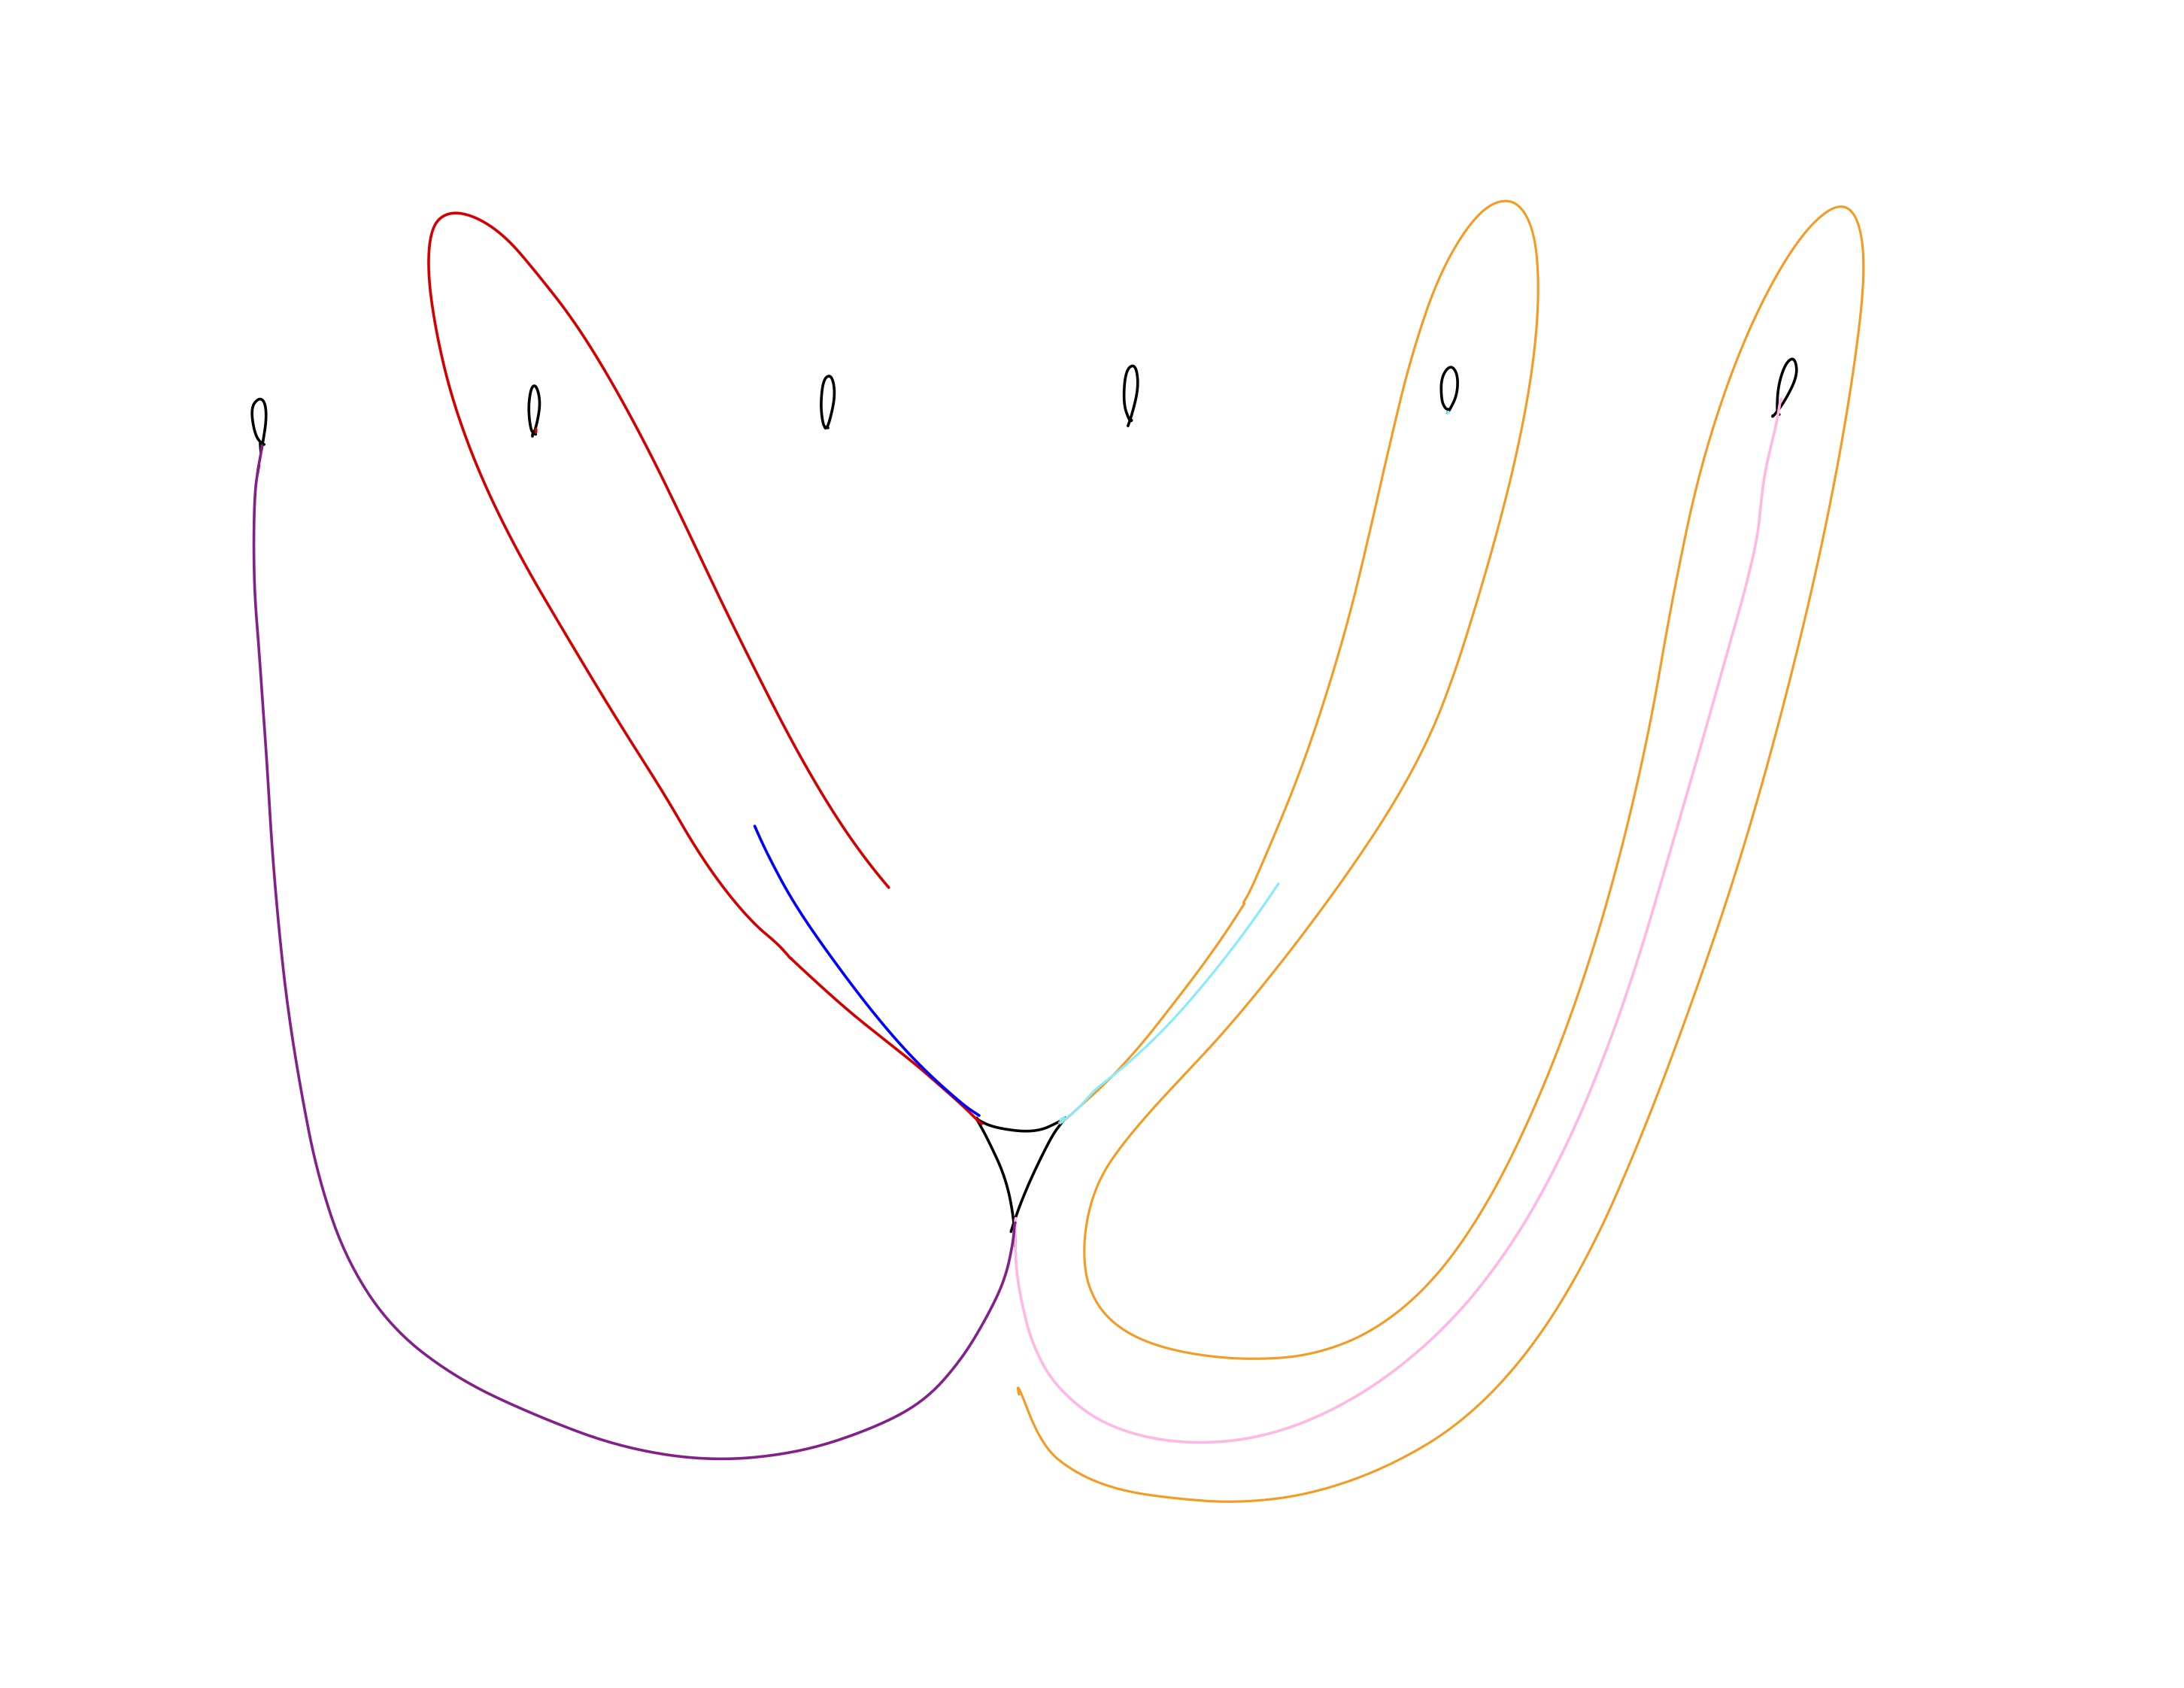
\includegraphics[width=\linewidth]{figures/Case Analysis Example Candelabra-05.jpg}
    \caption{Failure of the $\fbs = p^\circ$ and $\fbs = p^-$ branches: $\fbo$ is forced to begin with $p^-$ and is absorbed between $\fbp$ and $\fbi$.}
    \label{fig:Jehu_example_5}
\end{figure}

We must therefore have instead $\fbs = p^+\ldots$, and the next letter can be either $o^{*}$ or $s^{*}$. To avoid tracing, it must be the former:
\[
\fbs = p^+ o^*\ldots.
\]
This is Figure \ref{fig:Jehu_example_6}. Note that $\fbs$ must go to the left of $\fbr$; otherwise $\fbs$ would continue traversing the outer perimeter and be absorbed between $\fbp$ and $\fbi$.

\begin{figure}[H]
    \centering
    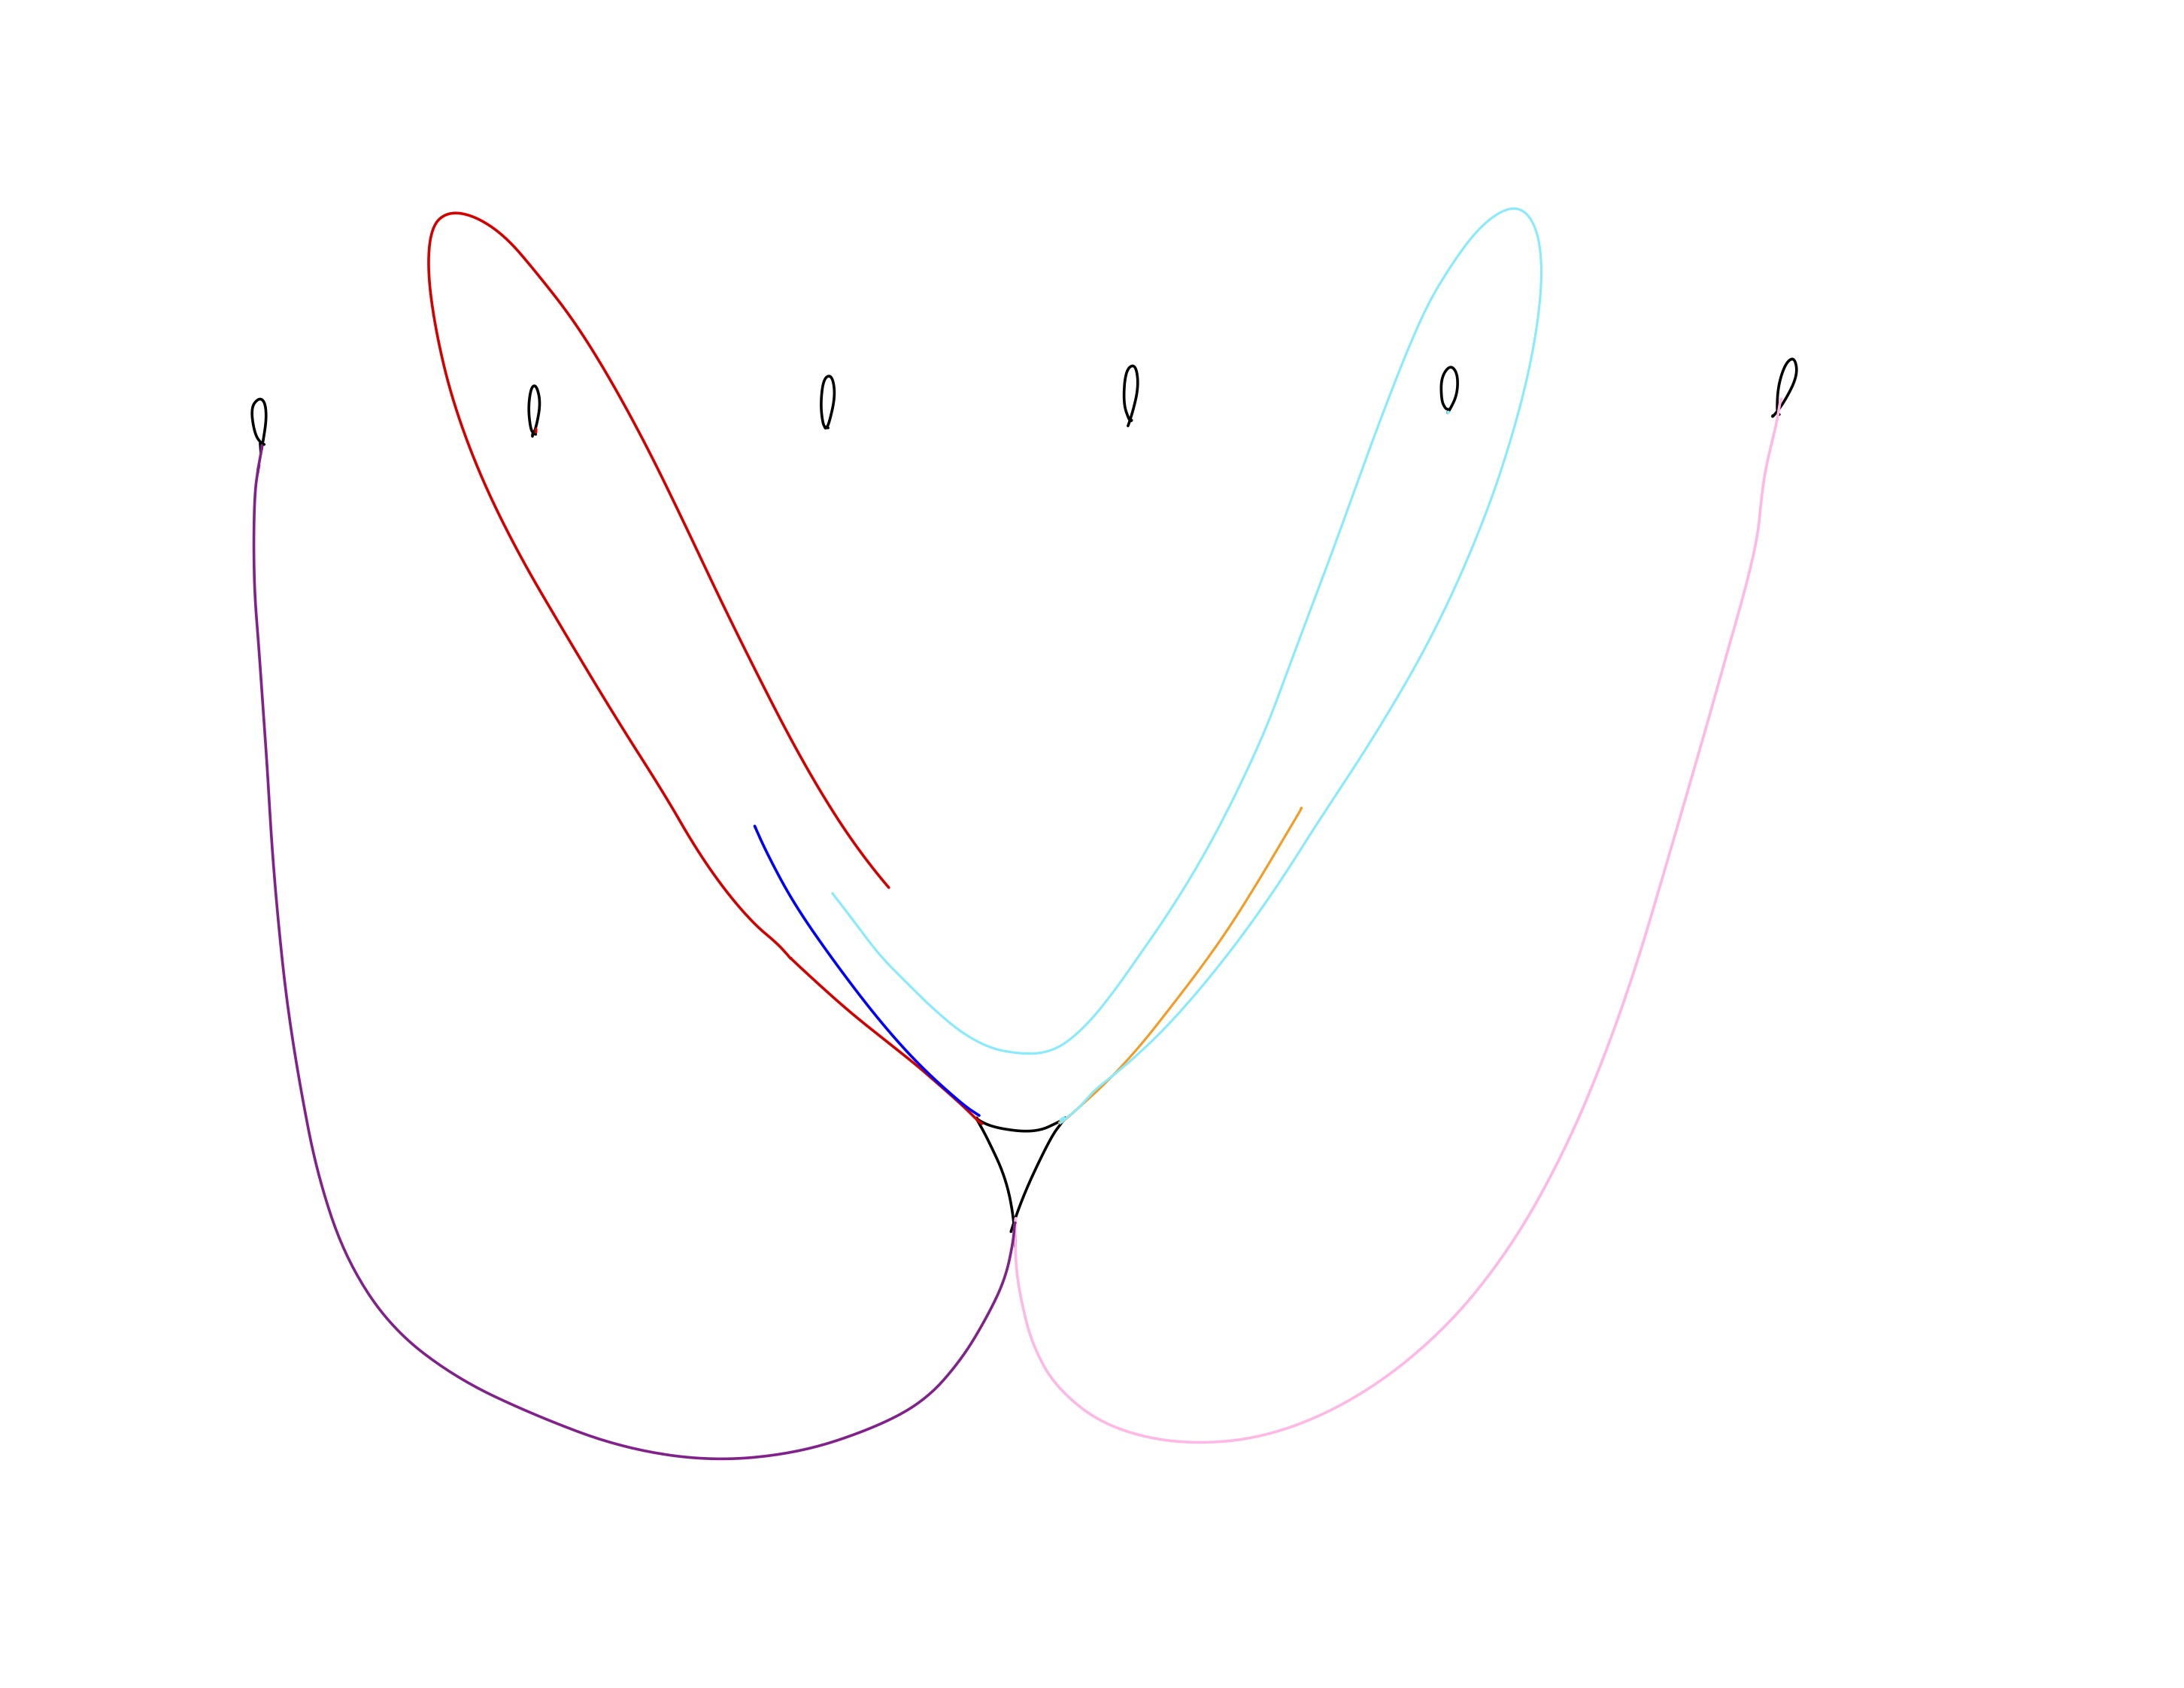
\includegraphics[width=\linewidth]{figures/Case Analysis Example Candelabra-06.jpg}
    \caption{Forced continuation: $\fbs = p^+ o^*\ldots$, with $\fbs$ passing to the left of $\fbr$ to avoid the outer-perimeter absorption.}
    \label{fig:Jehu_example_6}
\end{figure}

We can now return to $\fbr$. In this situation, if $\fbr$ continued with $p^*$, then it would traverse above $\fbs$ and wrap around to be absorbed:
\[
\fbr = o^- p^- r^- \Abso{\fbp}{\fbi},
\]
as shown in Figure \ref{fig:Jehu_example_7}.

\begin{figure}[H]
    \centering
    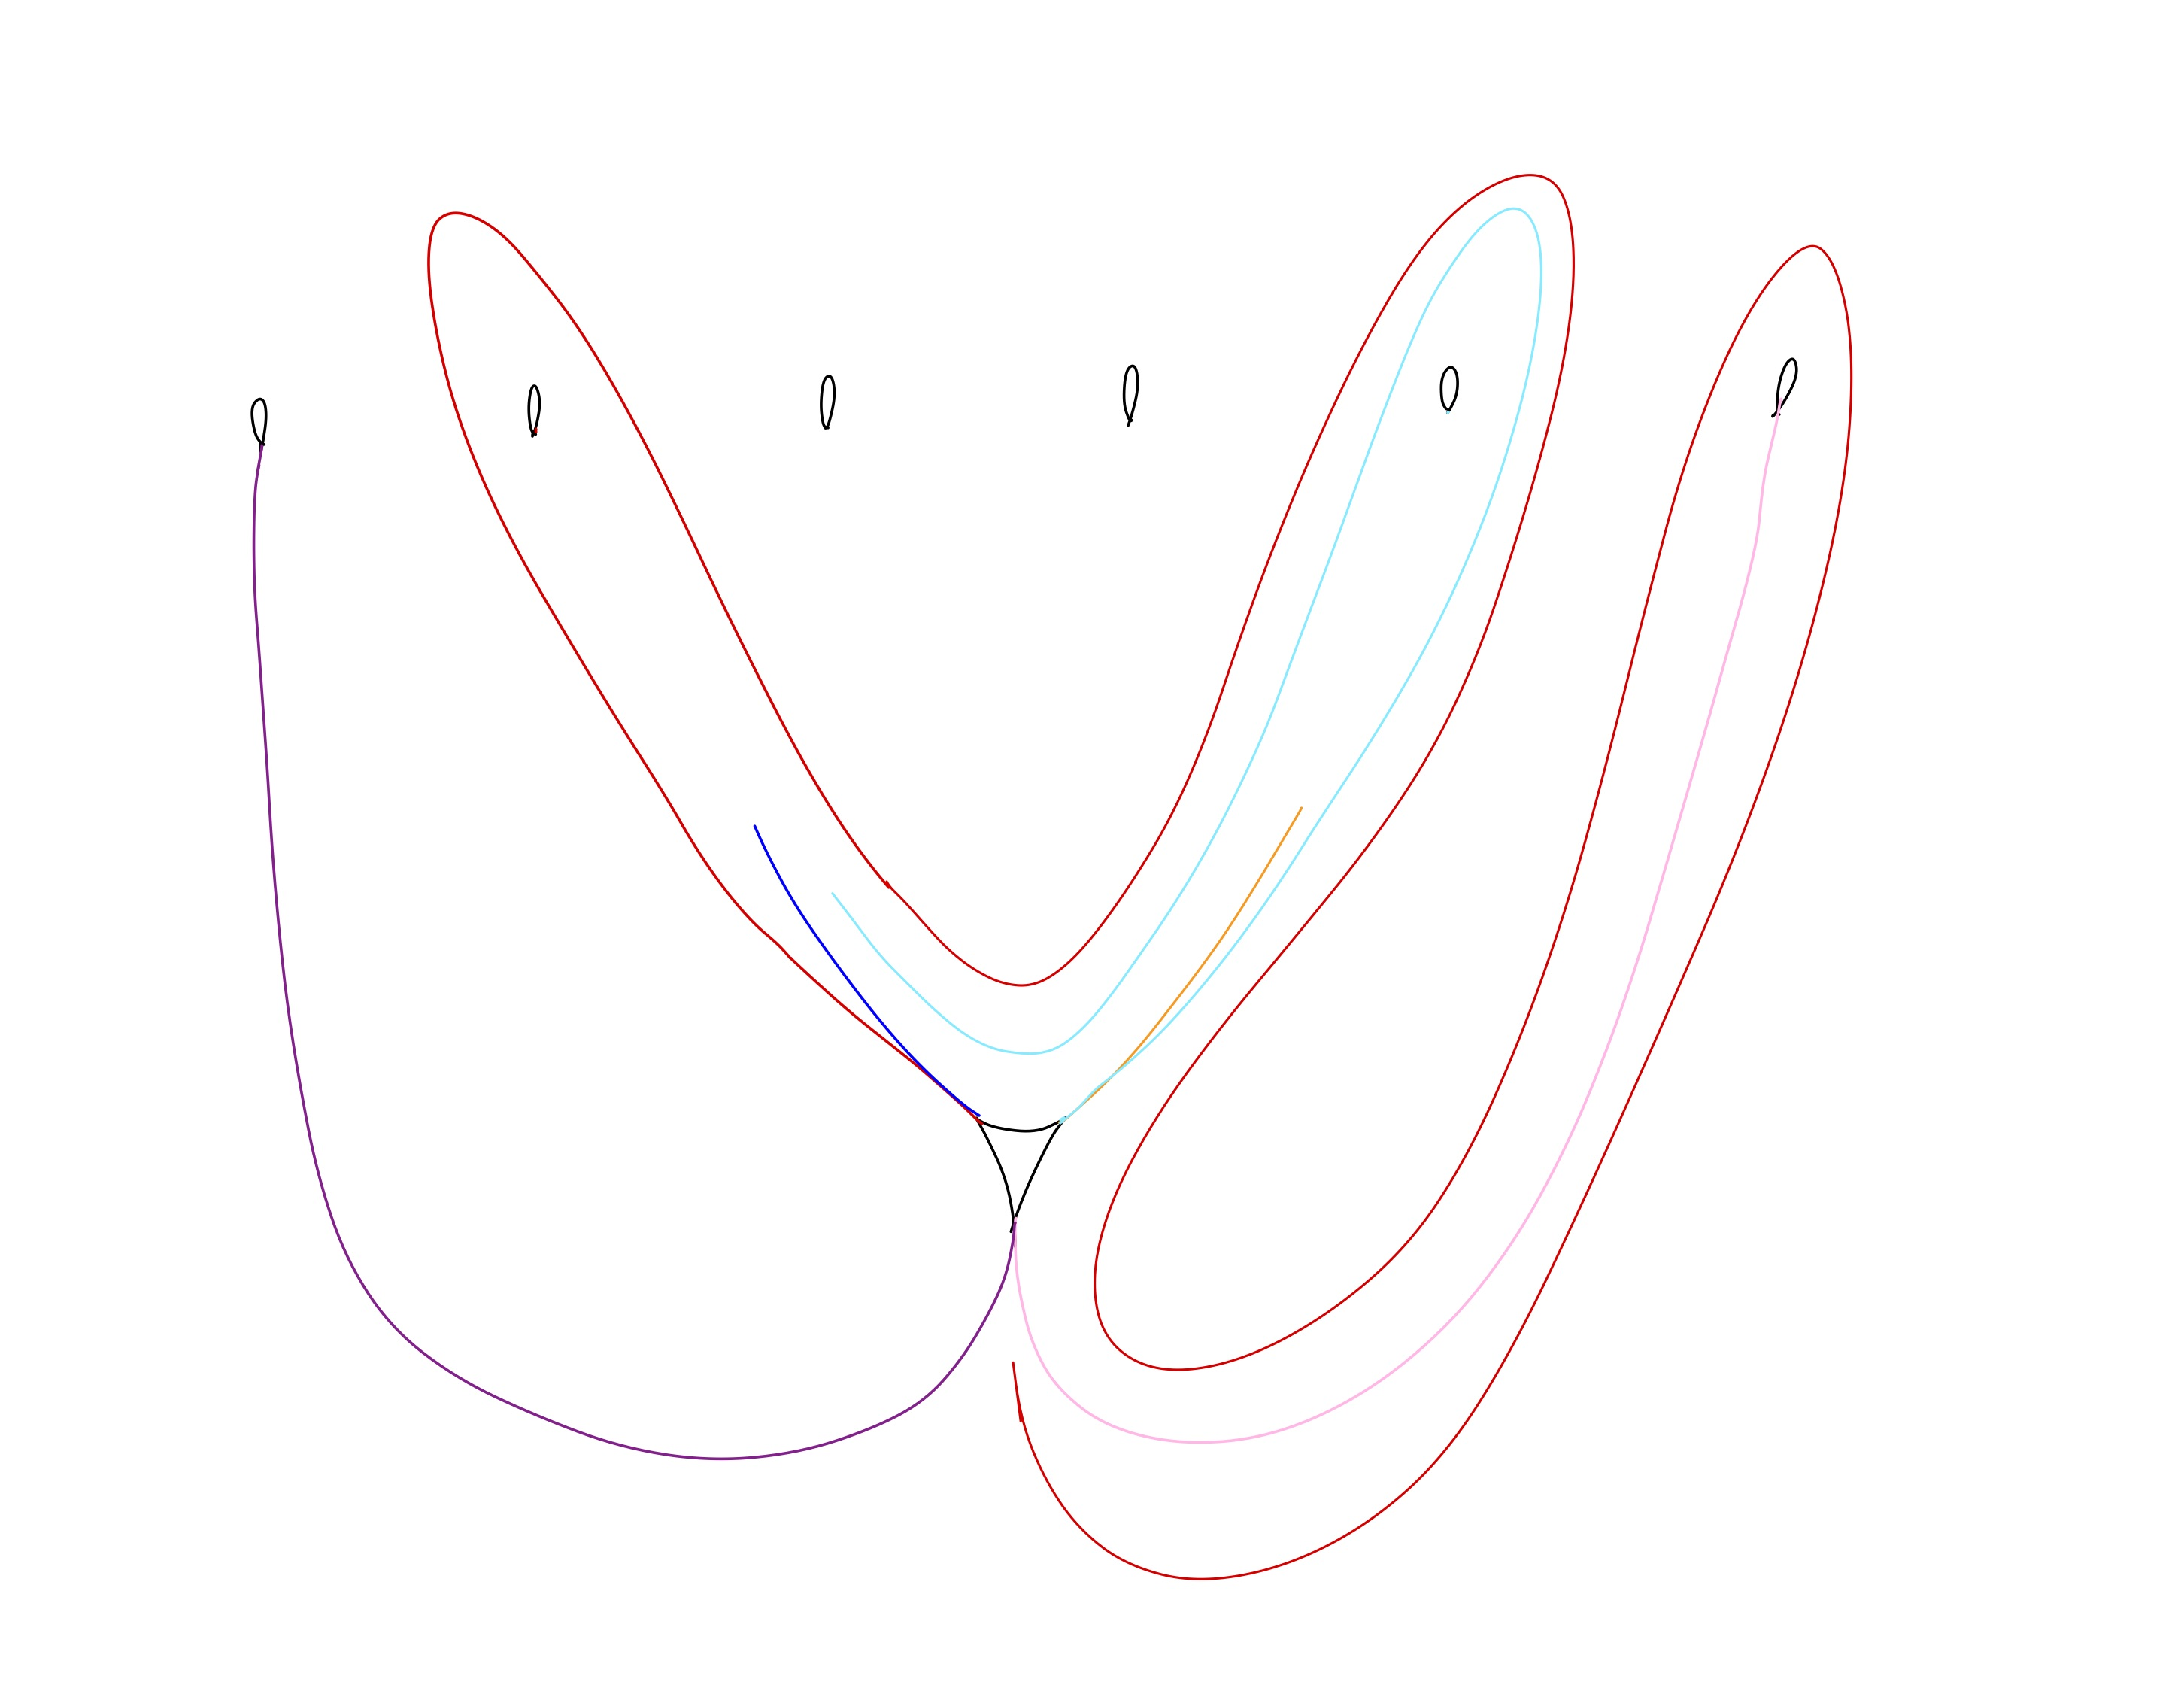
\includegraphics[width=\linewidth]{figures/Case Analysis Example Candelabra-07.jpg}
    \caption{Failure of the $\fbr = o^- p^*\ldots$ branch: $\fbr$ traverses above $\fbs$, wraps around $r^-$, and is absorbed between $\fbp$ and $\fbi$.}
    \label{fig:Jehu_example_7}
\end{figure}

We must therefore have
\[
\fbr = o^- i^*\ldots,
\]
as shown in Figure \ref{fig:Jehu_example_8}.

\begin{figure}[H]
    \centering
    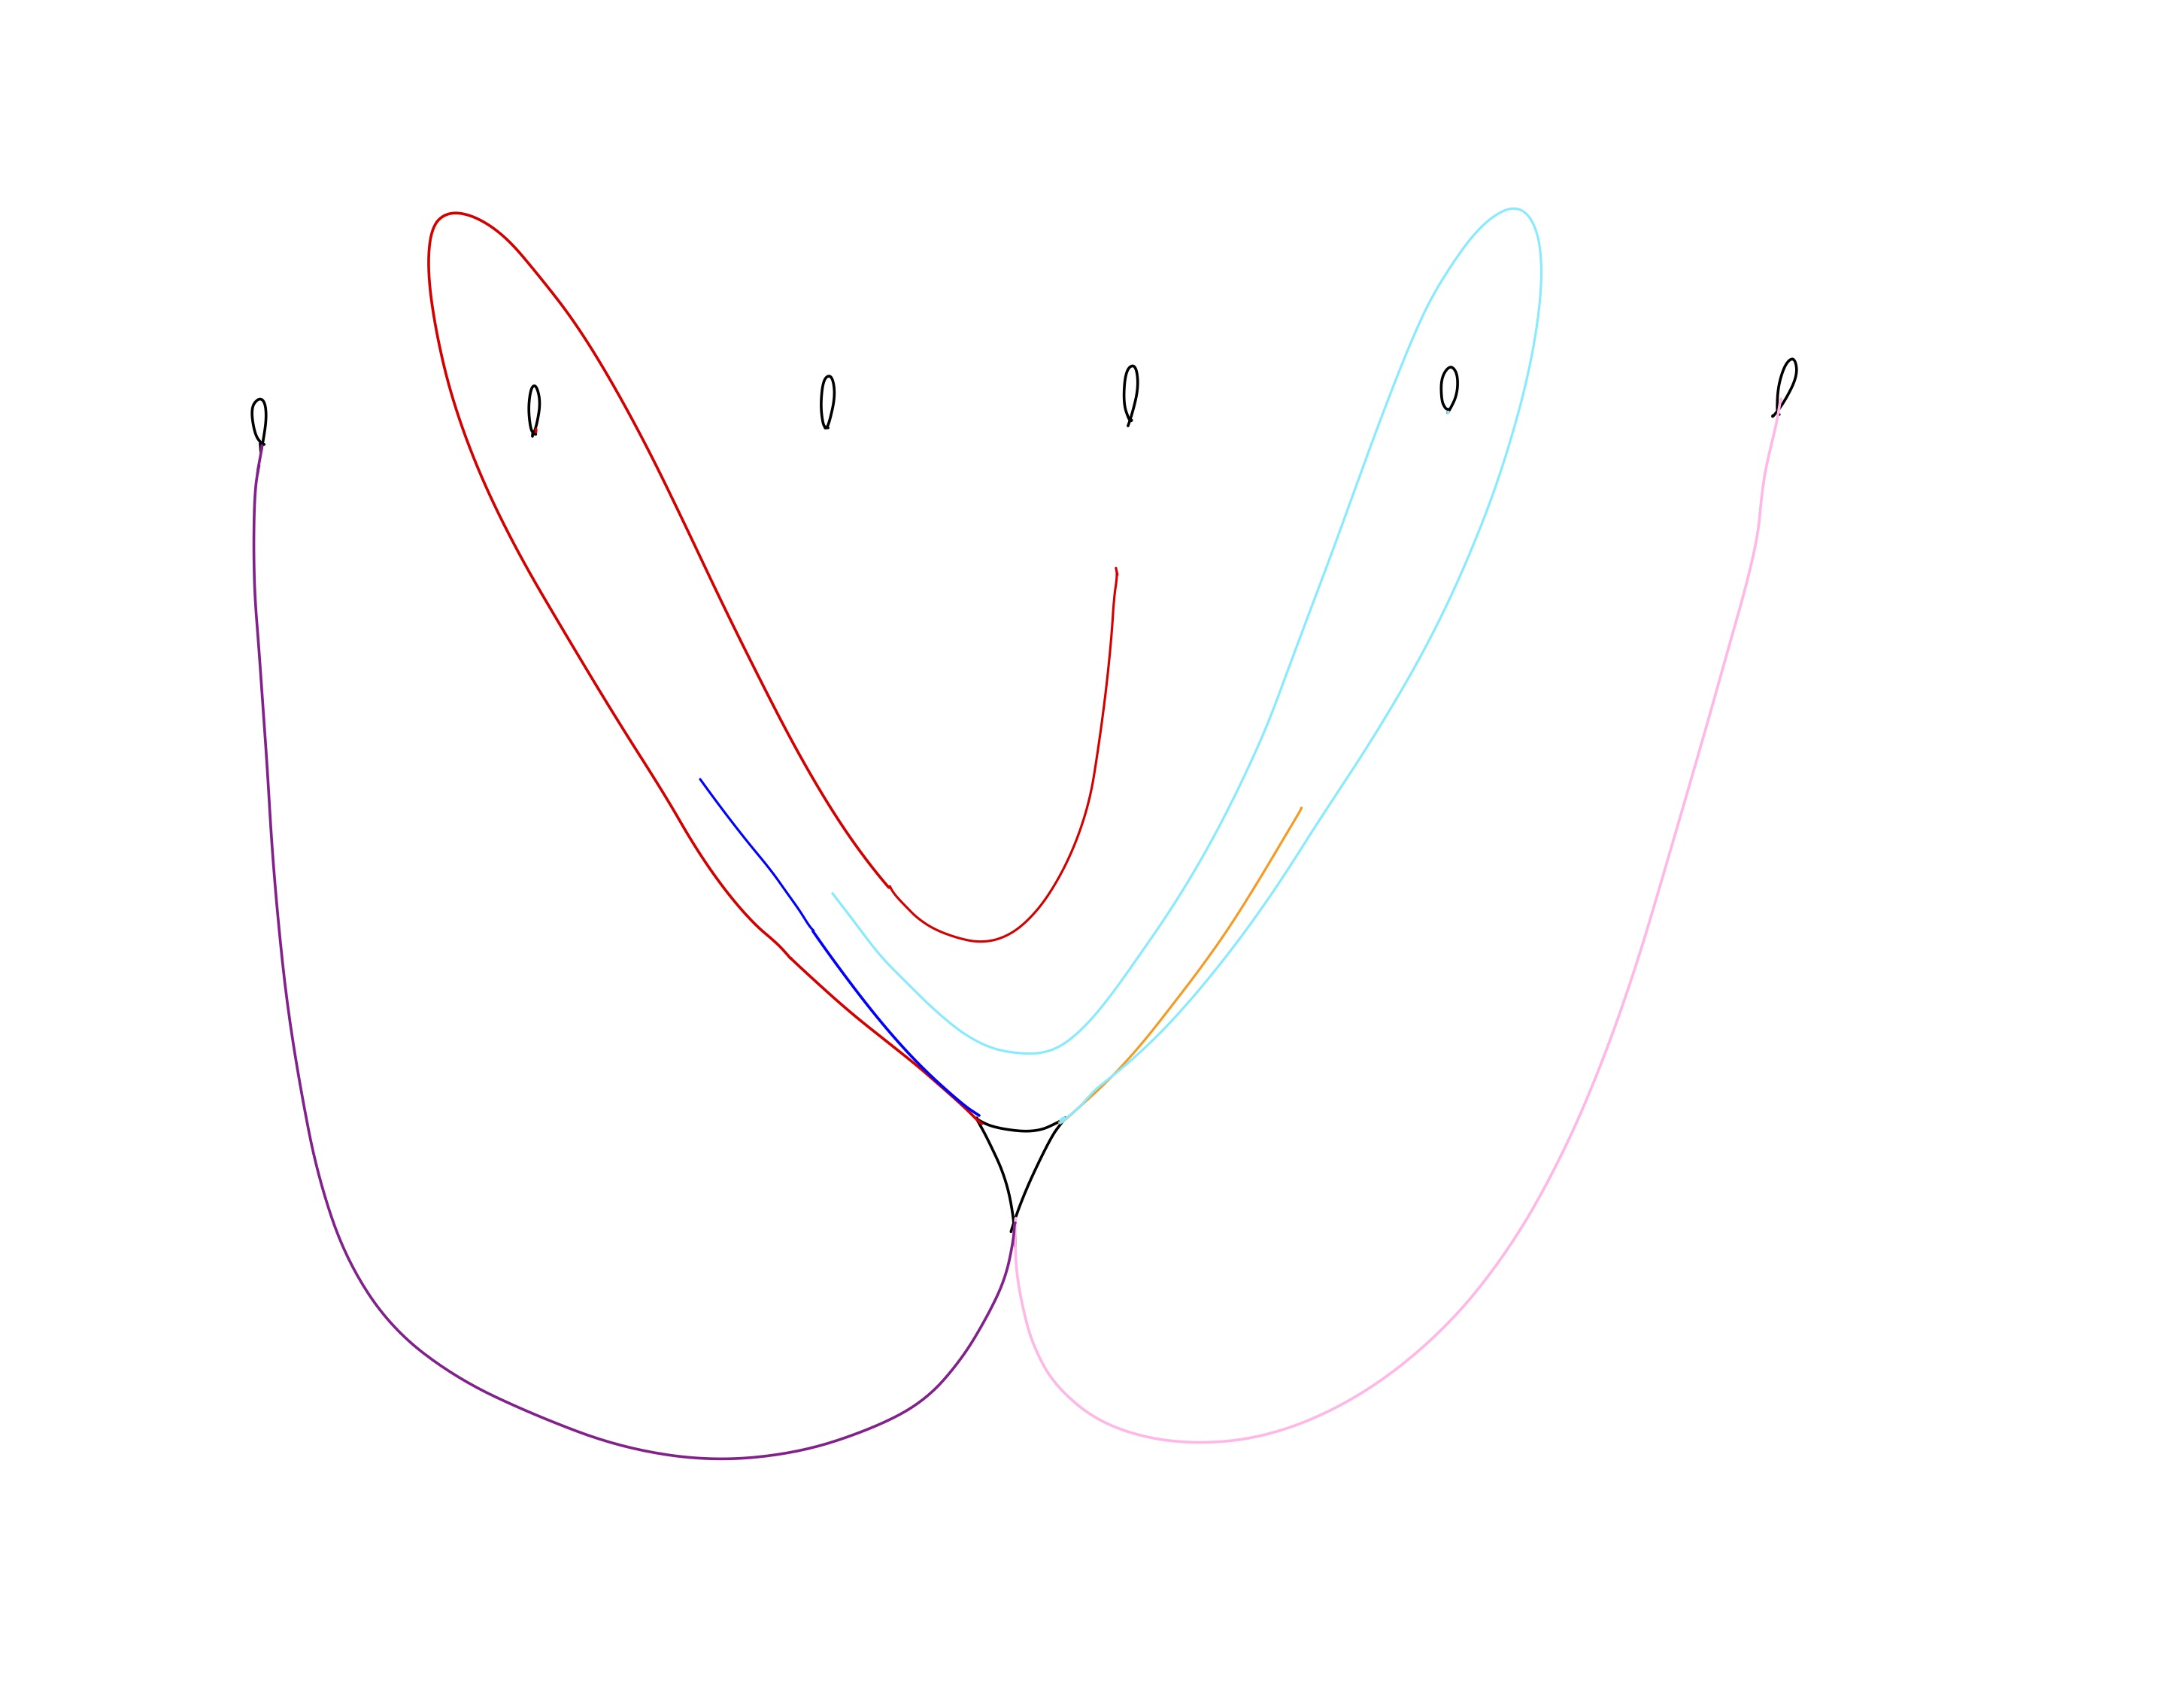
\includegraphics[width=\linewidth]{figures/Case Analysis Example Candelabra-08.jpg}
    \caption{Forced continuation: $\fbr = o^- i^*\ldots$, the only remaining admissible route.}
    \label{fig:Jehu_example_8}
\end{figure}

Now consider $\fbb$. Beginning with $o^+$ is ruled out by immediate absorption. On the other hand, if $\fbb$ began with $o^\circ$, the incoming $\fbs$ would then traverse $o^+$ and be absorbed. We must therefore have
\[
\fbb = o^- i^*\ldots,
\]
as shown in Figure \ref{fig:Jehu_example_9}.

\begin{figure}[H]
    \centering
    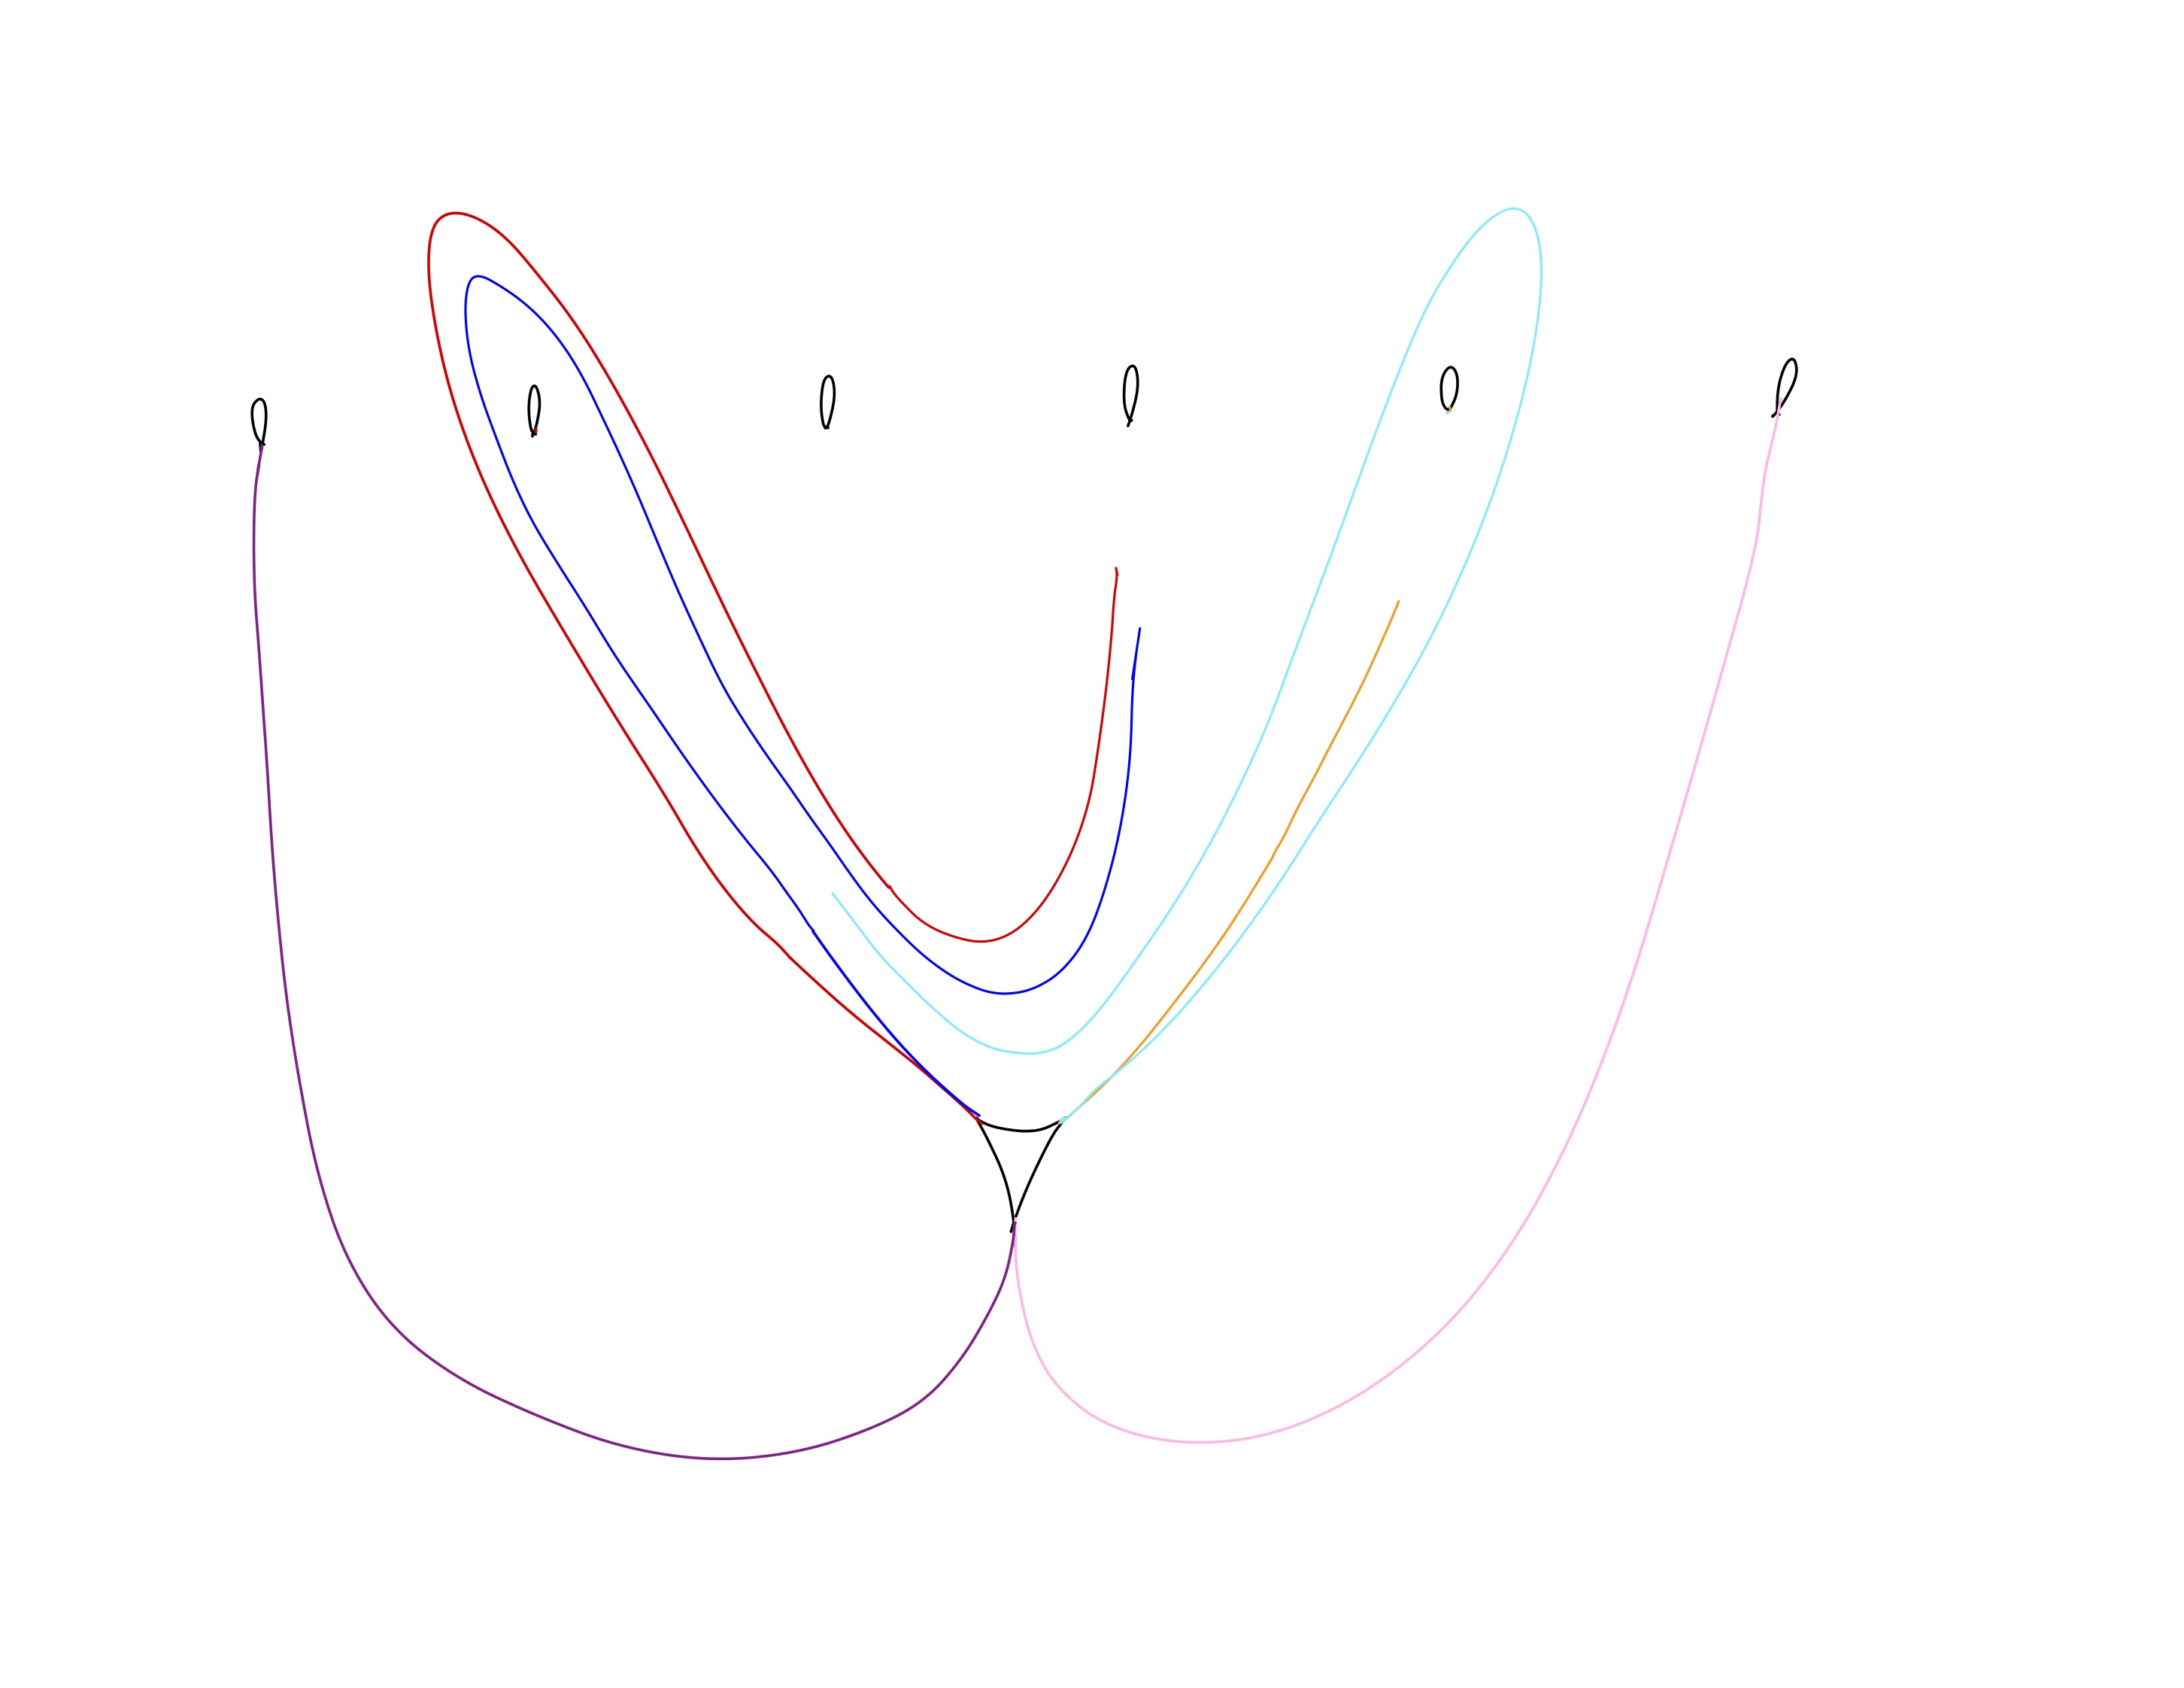
\includegraphics[width=\linewidth]{figures/Case Analysis Example Candelabra-09.jpg}
    \caption{Forced continuation: $\fbb = o^- i^*\ldots$, after ruling out $\fbb = o^+\ldots$ (immediate absorption) and $\fbb = o^\circ$ (which would absorb the incoming $\fbs$).}
    \label{fig:Jehu_example_9}
\end{figure}

Consider next the sub-branch in which $\fbs$ terminates at $o^\circ$:
\[
\fbs = p^+ o^\circ.
\]
(The complete case analysis verifies that if $\fbs$ did not terminate here, the resulting configuration would eventually produce a contradiction, but the argument requires extensive further branching that we omit.) The situation is shown in Figure \ref{fig:Jehu_example_10}.

\begin{figure}[H]
    \centering
    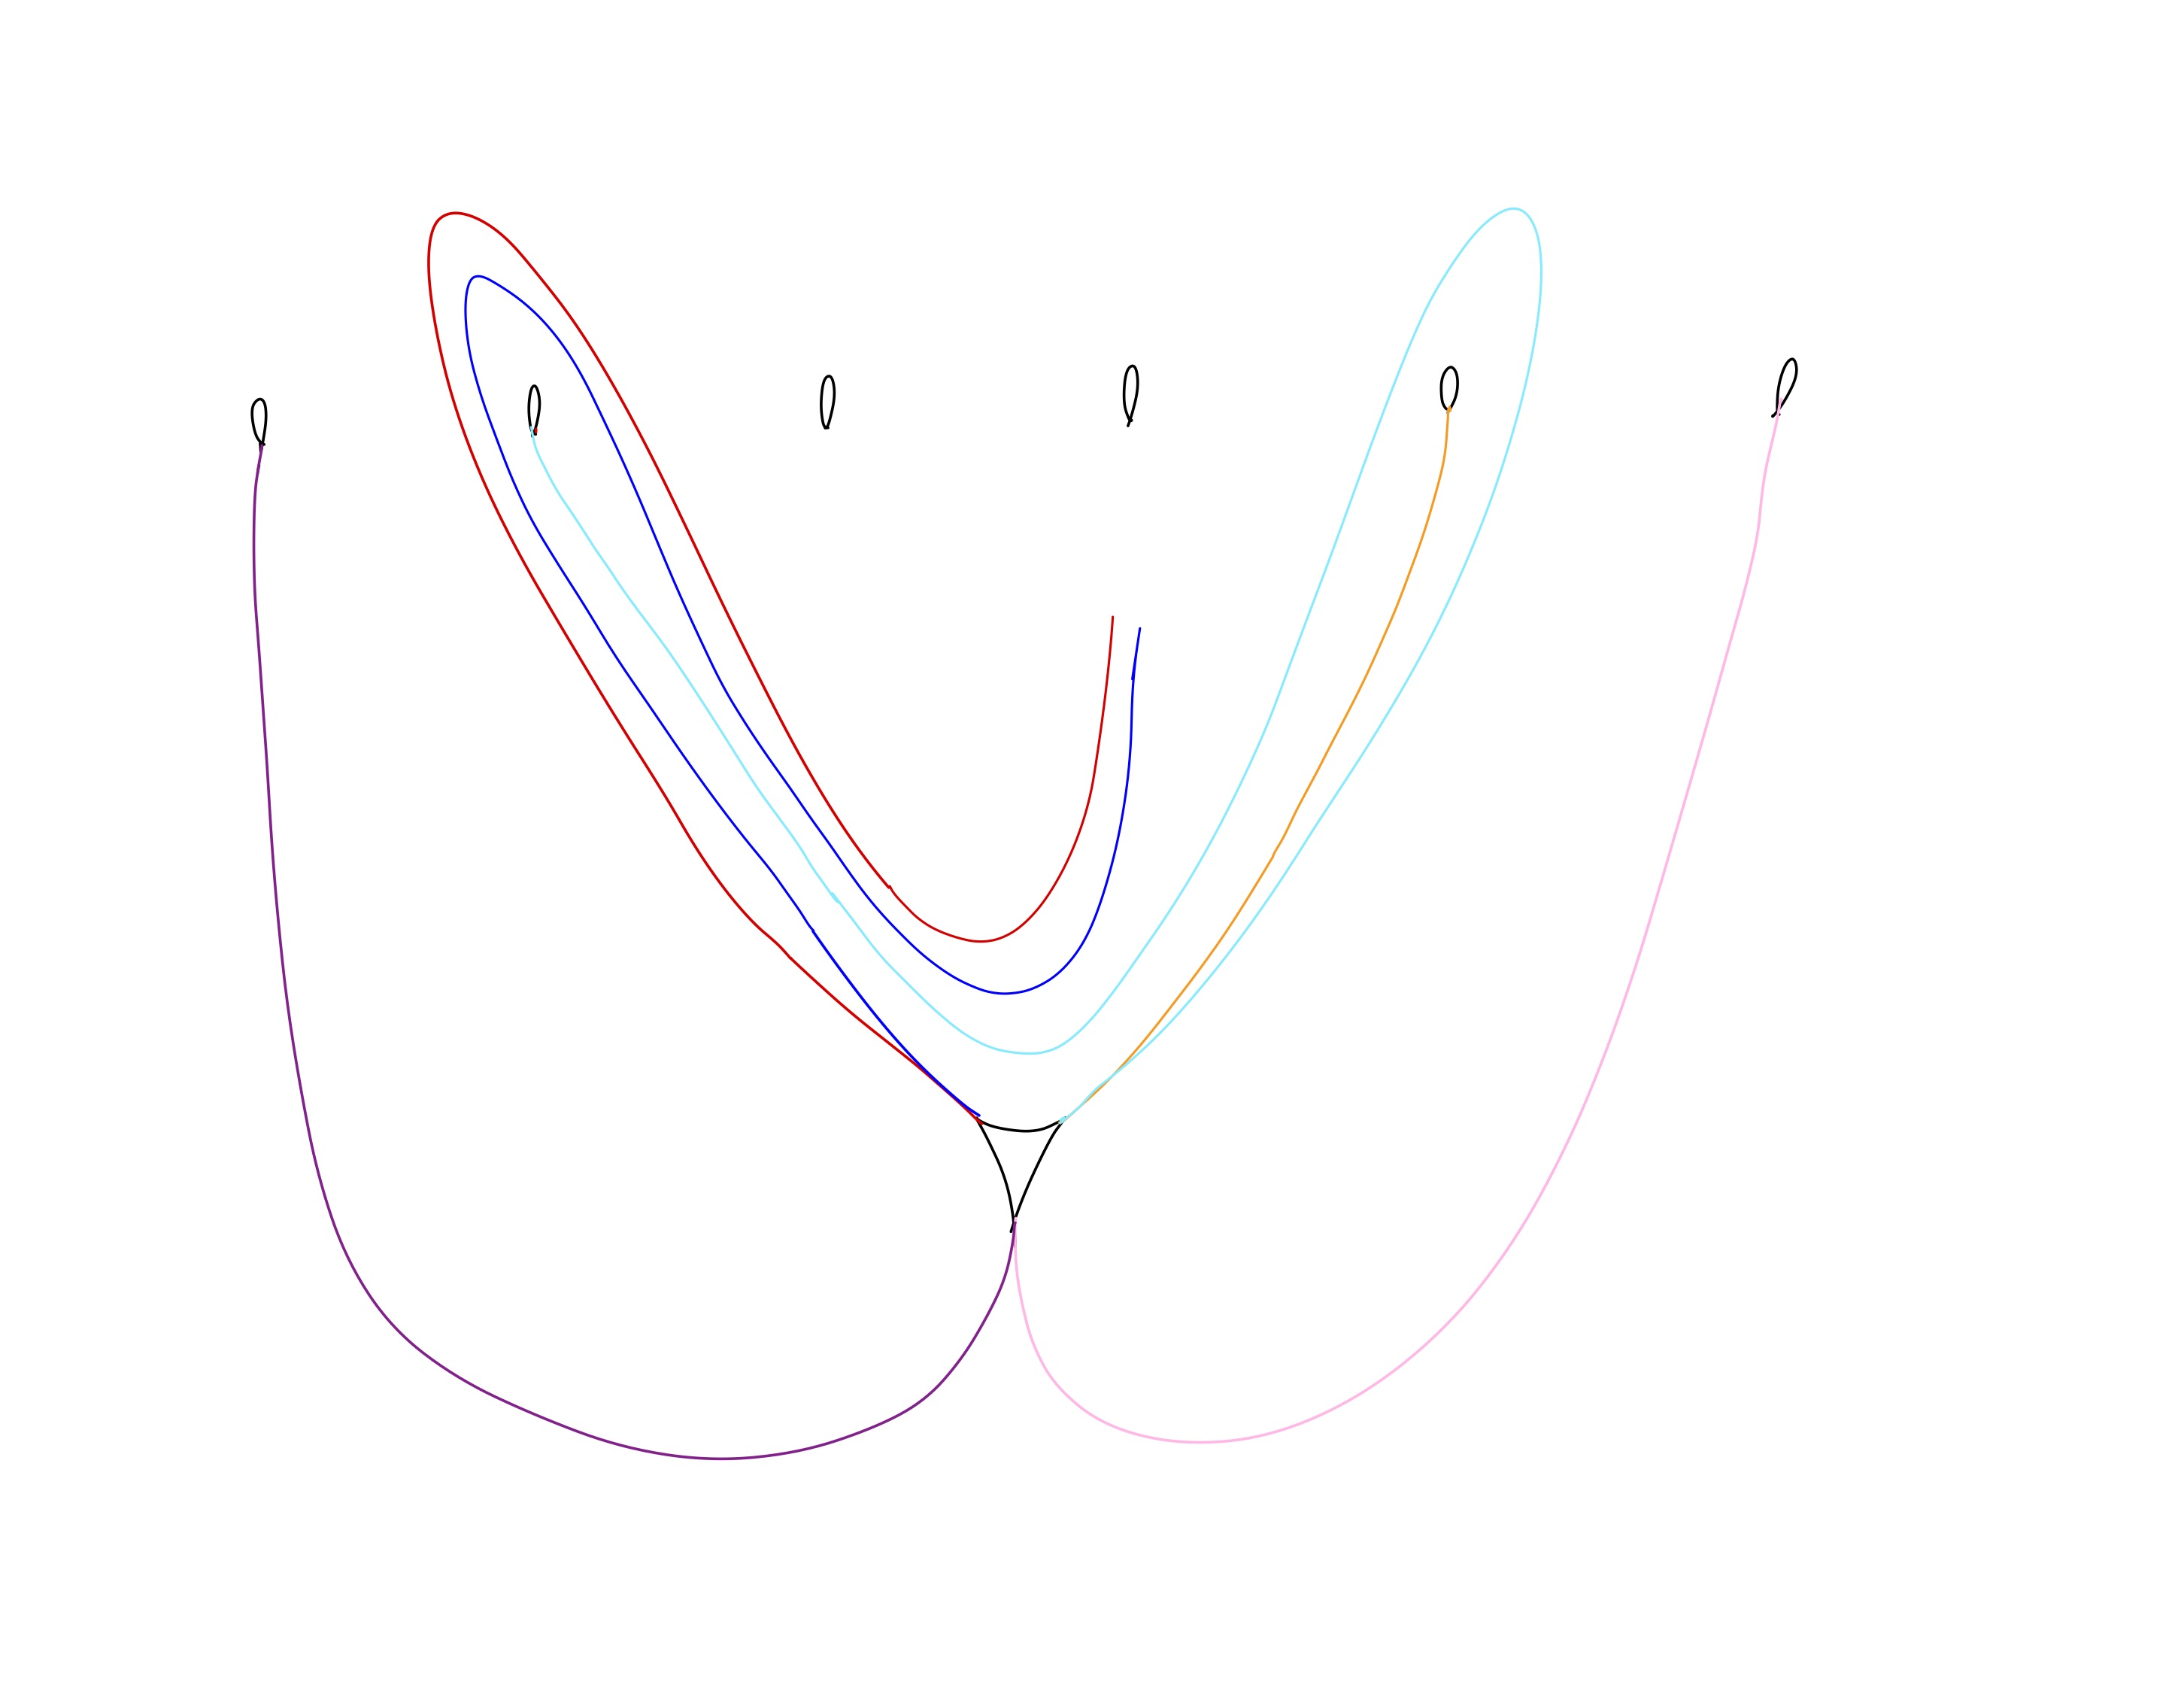
\includegraphics[width=\linewidth]{figures/Case Analysis Example Candelabra-10.jpg}
    \caption{The subcase $\fbs = p^+ o^\circ$ (terminating at $o$), together with the forced $\fbo = p^\circ$ in this configuration.}
    \label{fig:Jehu_example_10}
\end{figure}

In this situation, $\fbo$ must terminate immediately: if it did not, the next letter could only be $o^*$, which would trace. Thus
\[
\fbo = p^\circ.
\]
It remains to determine the continuations of $\fbb$ and $\fbr$. Here $\fbb$ cannot continue with $i^\circ$ or $i^-$: either choice would force $\fbr$ to continue with $i^-$, which would then be absorbed:
\[
\fbr = o^- i^- o^+ p^- \Abso{\fbo}{\fbs},
\]
as shown in Figure \ref{fig:Jehu_example_11}.

\begin{figure}[H]
    \centering
    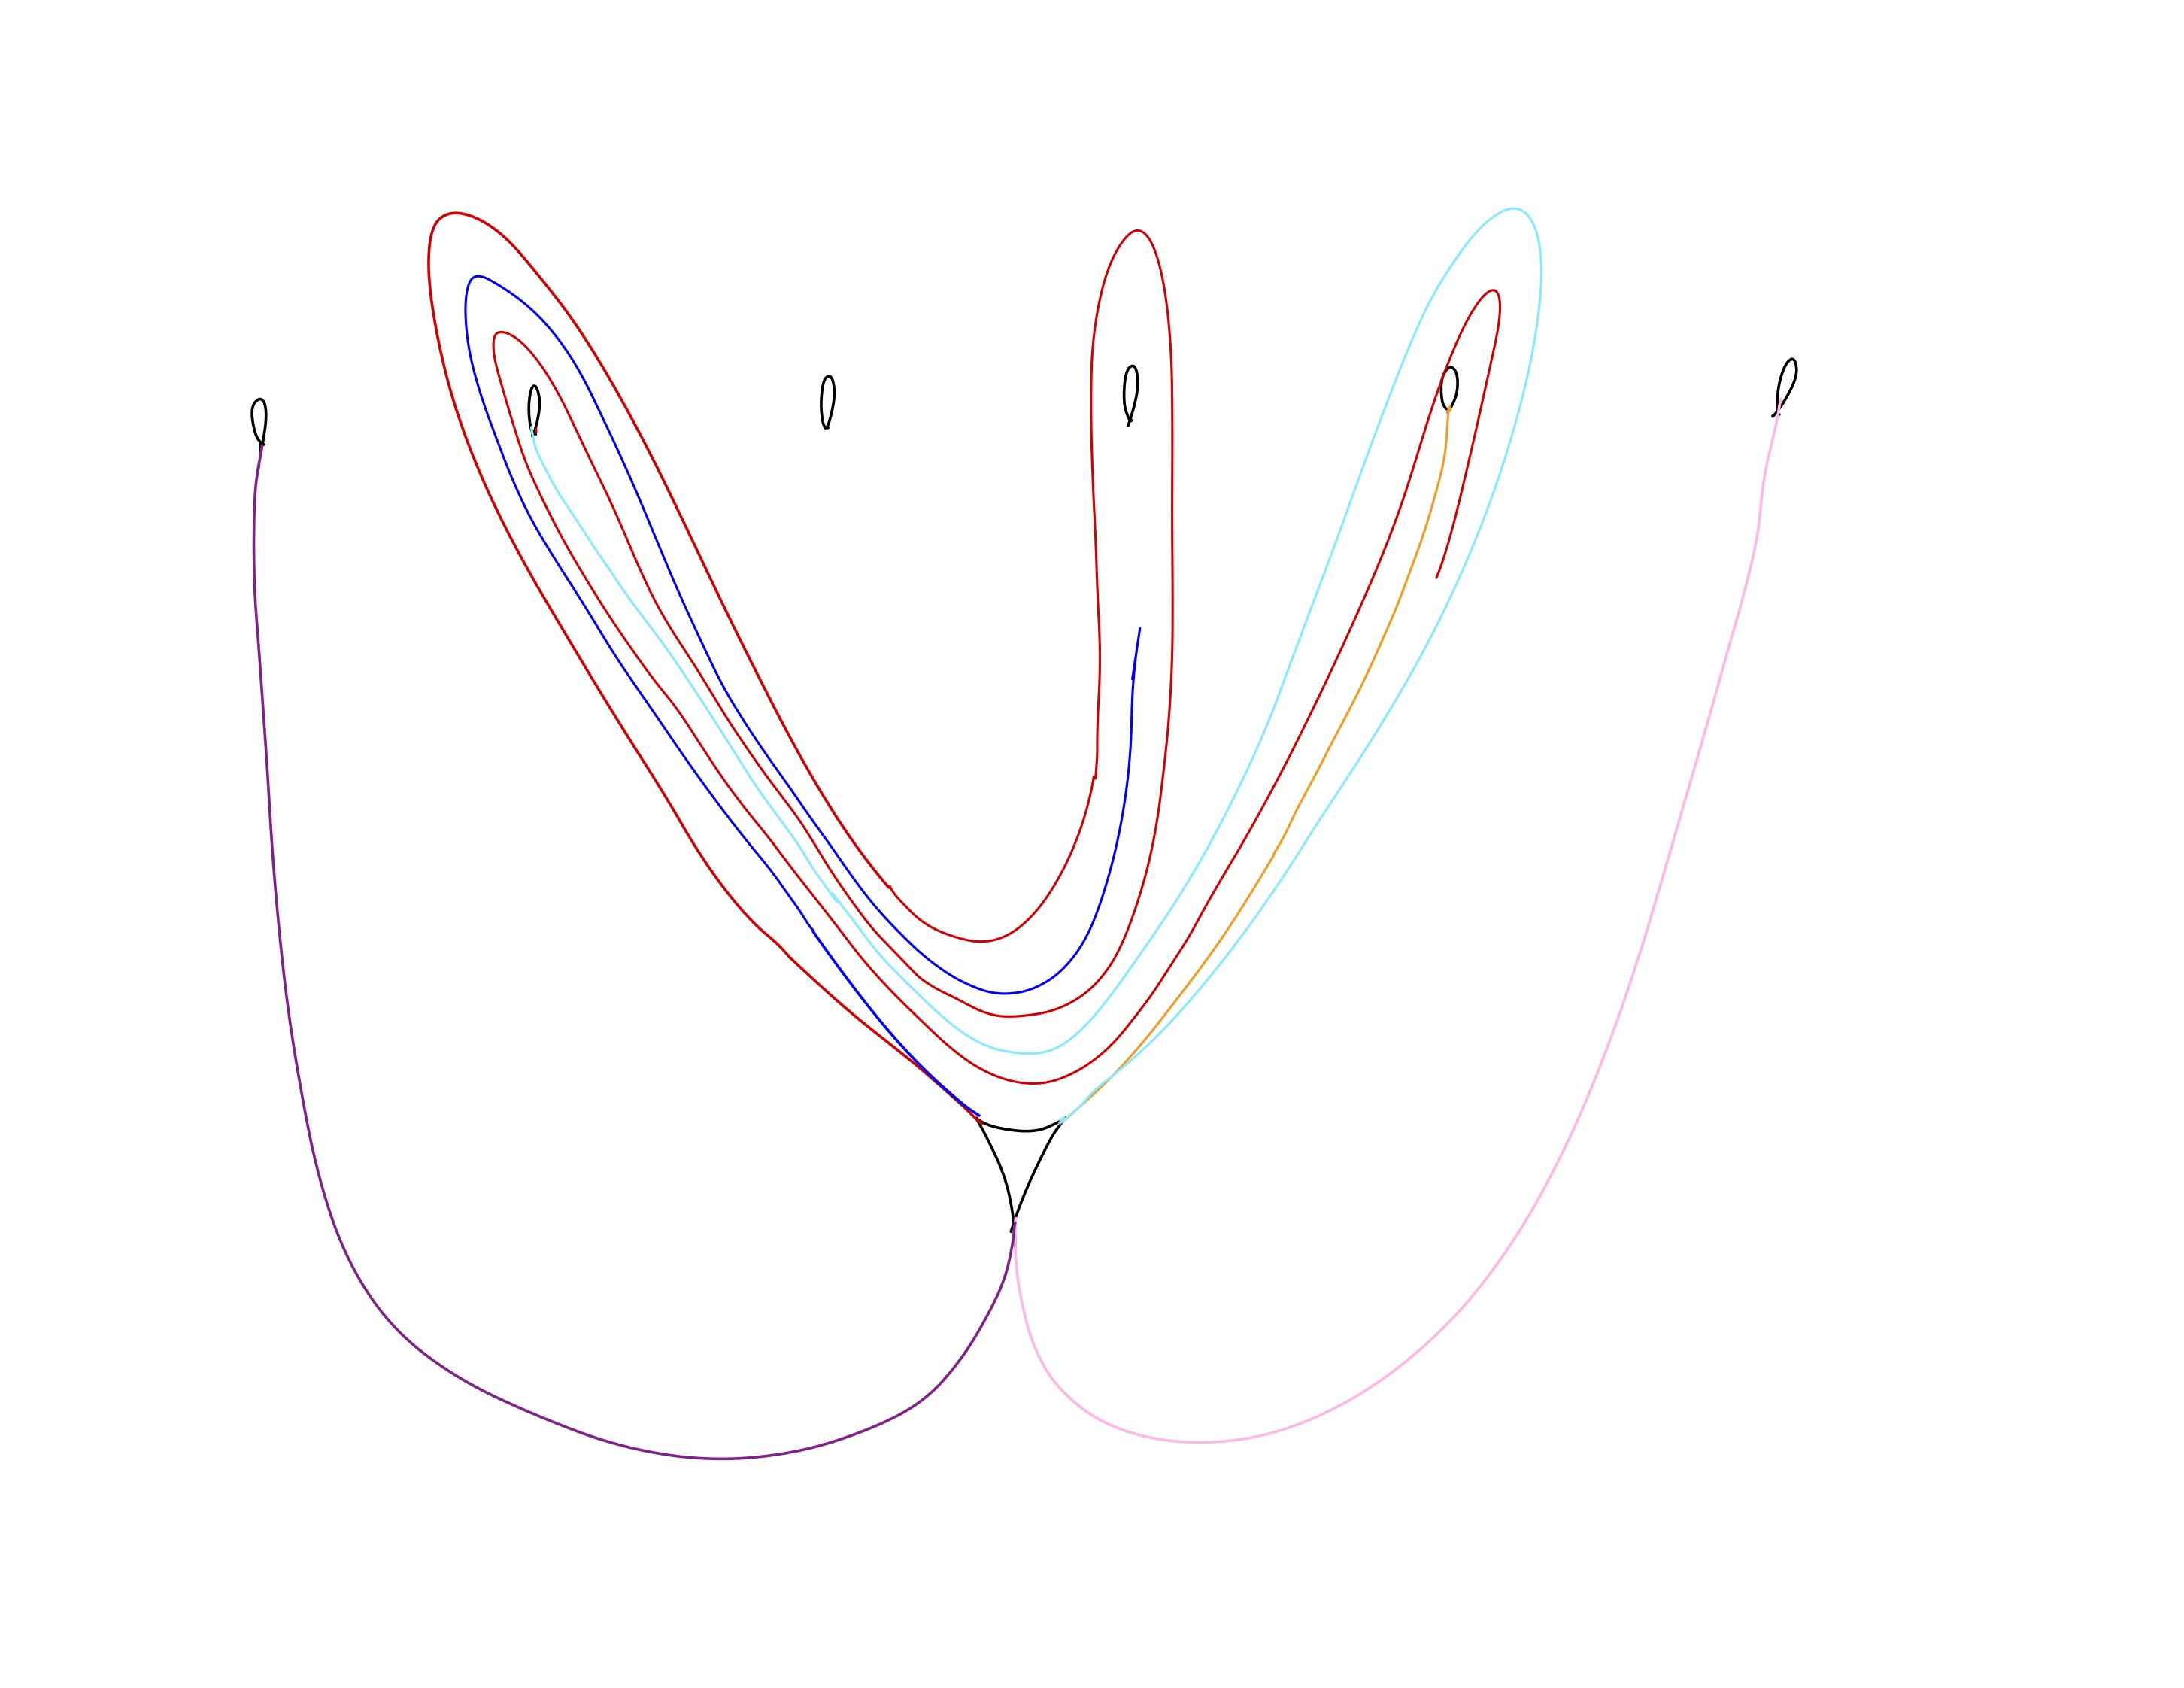
\includegraphics[width=\linewidth]{figures/Case Analysis Example Candelabra-11.jpg}
    \caption{Failure of the $\fbb = o^- i^\circ$ and $\fbb = o^- i^-$ branches: $\fbr$ is forced into $o^- i^- o^+ p^-$ and absorbed between $\fbo$ and $\fbs$.}
    \label{fig:Jehu_example_11}
\end{figure}

We must therefore have
\[
\fbb = o^- i^+ s^*\ldots,
\]
as shown in Figure \ref{fig:Jehu_example_12}.

\begin{figure}[H]
    \centering
    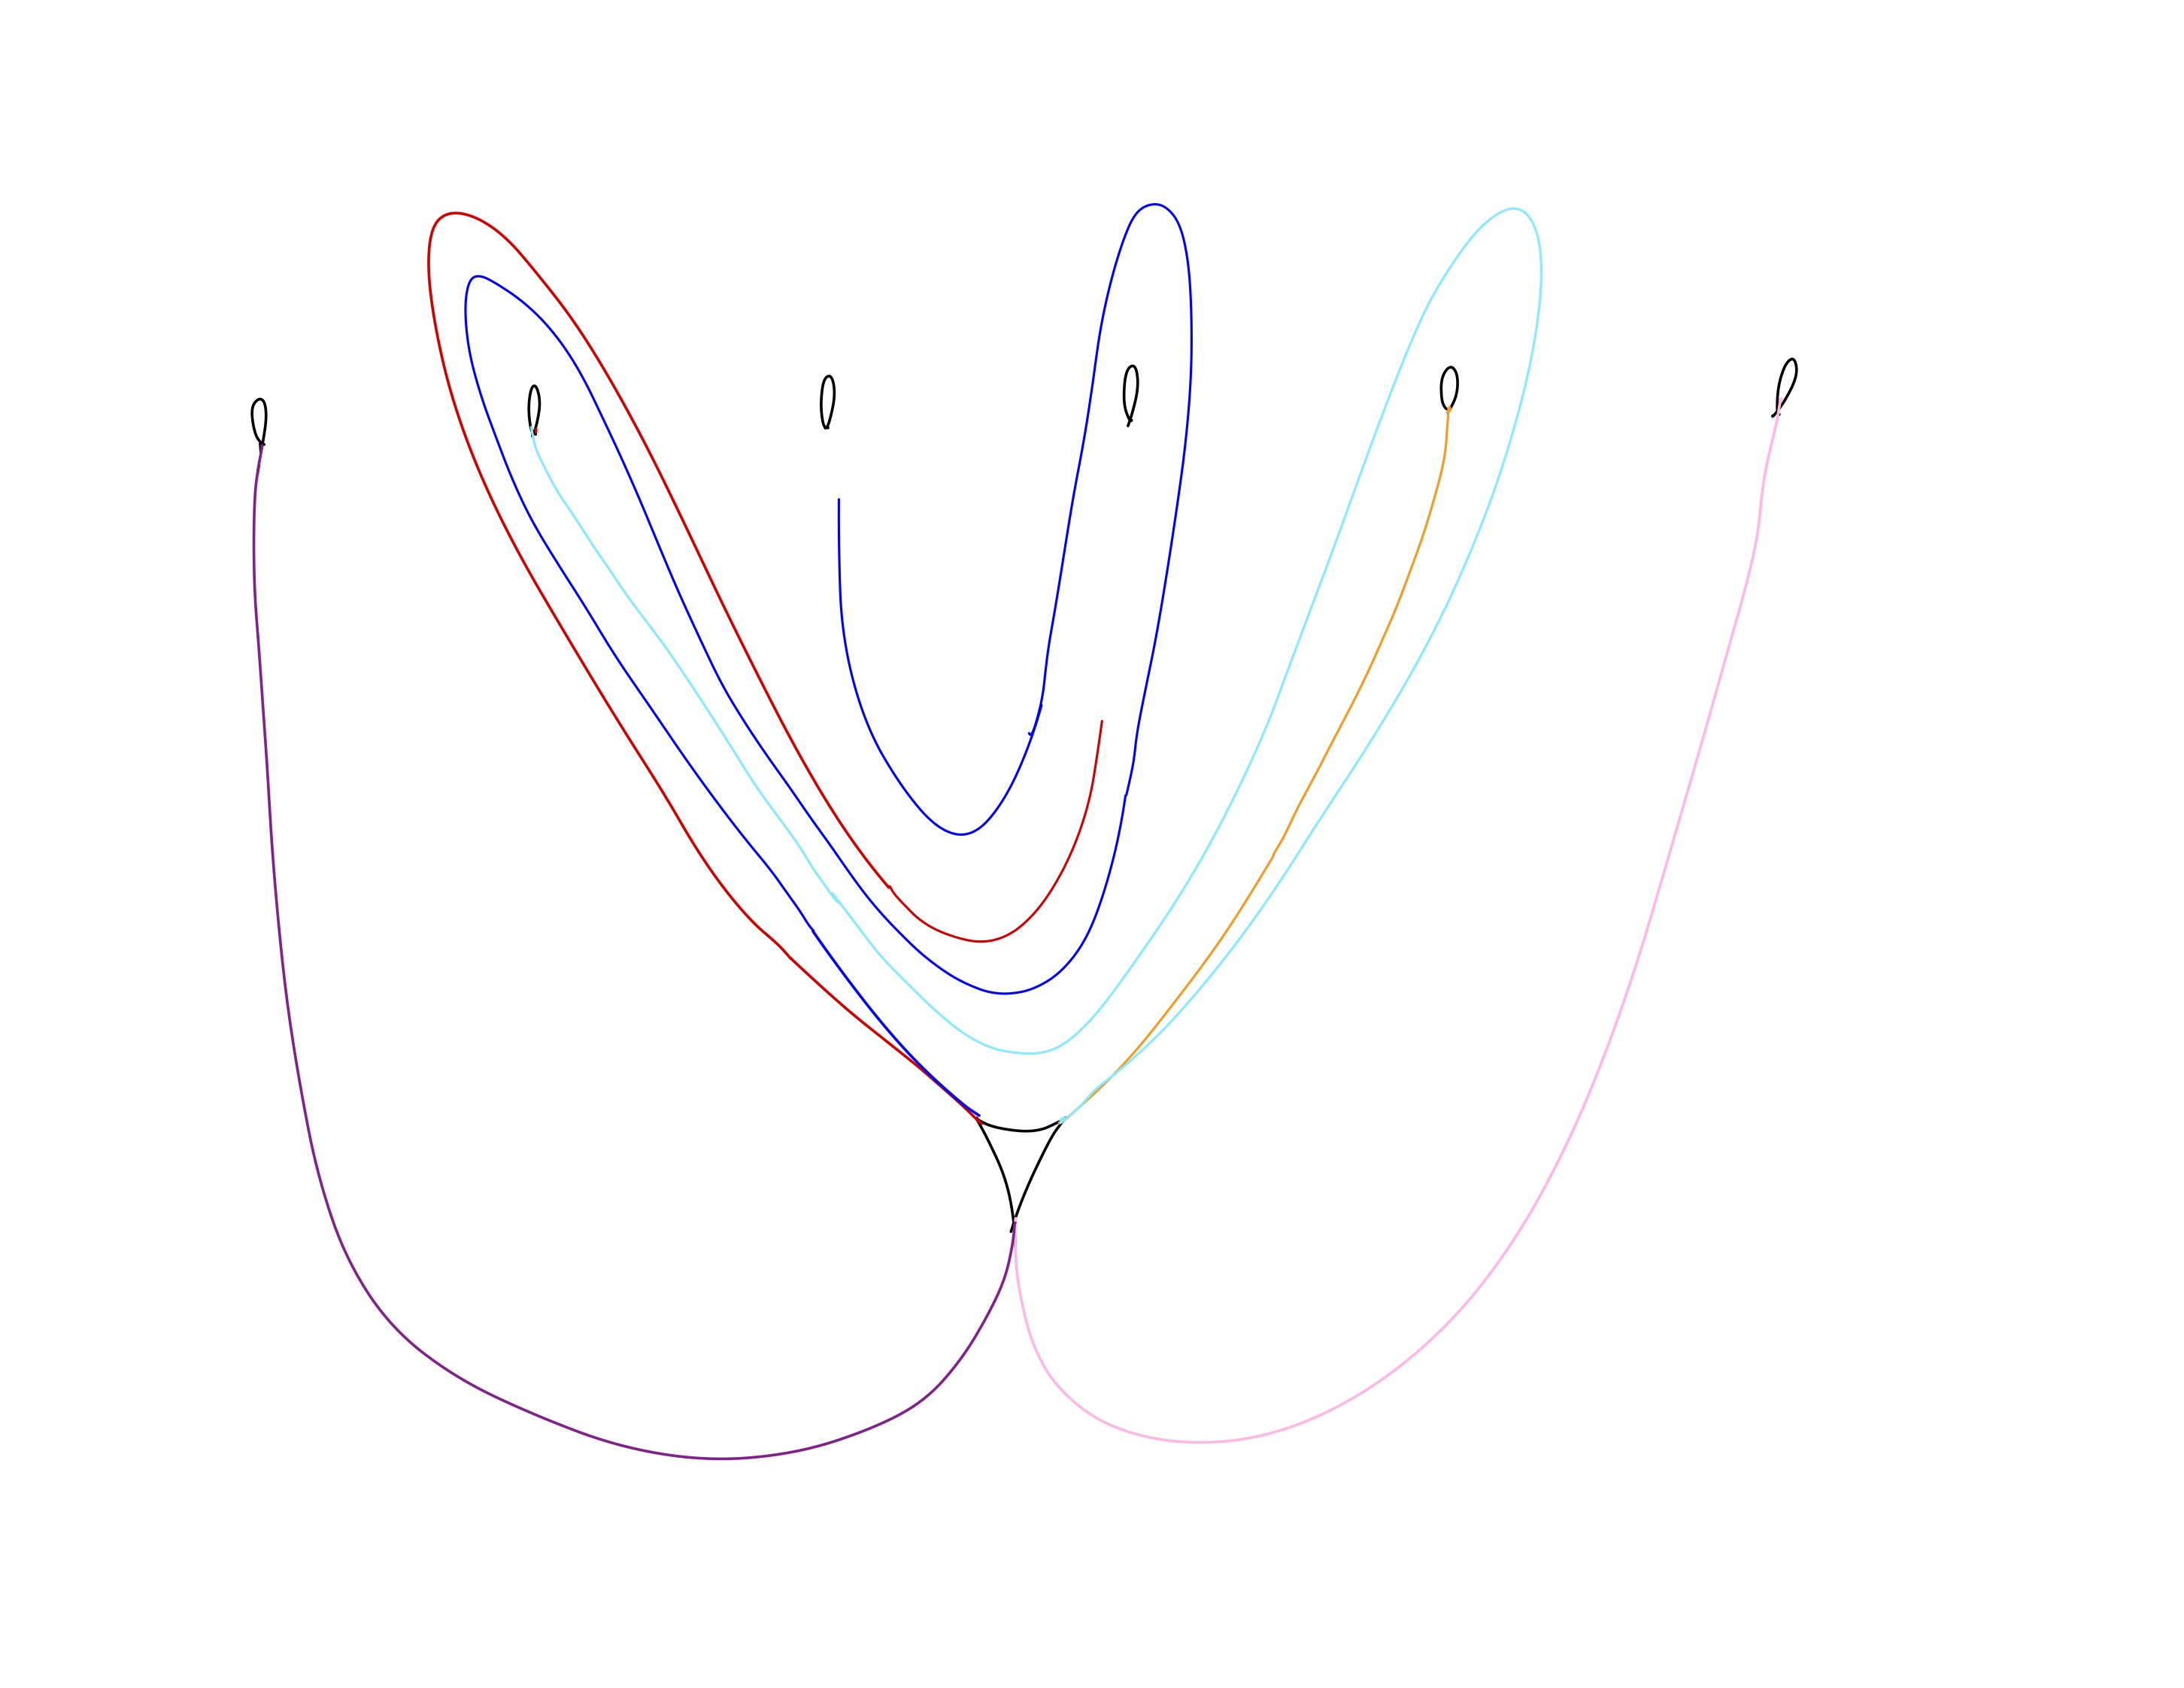
\includegraphics[width=\linewidth]{figures/Case Analysis Example Candelabra-12.jpg}
    \caption{Forced continuation: $\fbb = o^- i^+ s^*\ldots$, the only remaining admissible route.}
    \label{fig:Jehu_example_12}
\end{figure}

At this point, $\fbb$ and $\fbr$ may both terminate, or they may twist between $s^*$ and $i^*$ some number of times before terminating. Figures \ref{fig:Jehu_example_13} and \ref{fig:Jehu_example_14} show two examples of such twisting. Neither $\fbb$ nor $\fbr$ can escape this region between $s$ and $i$ without eventually being absorbed or tracing; both must terminate at one of the two letters after finitely many twists.

\begin{figure}[H]
    \centering
    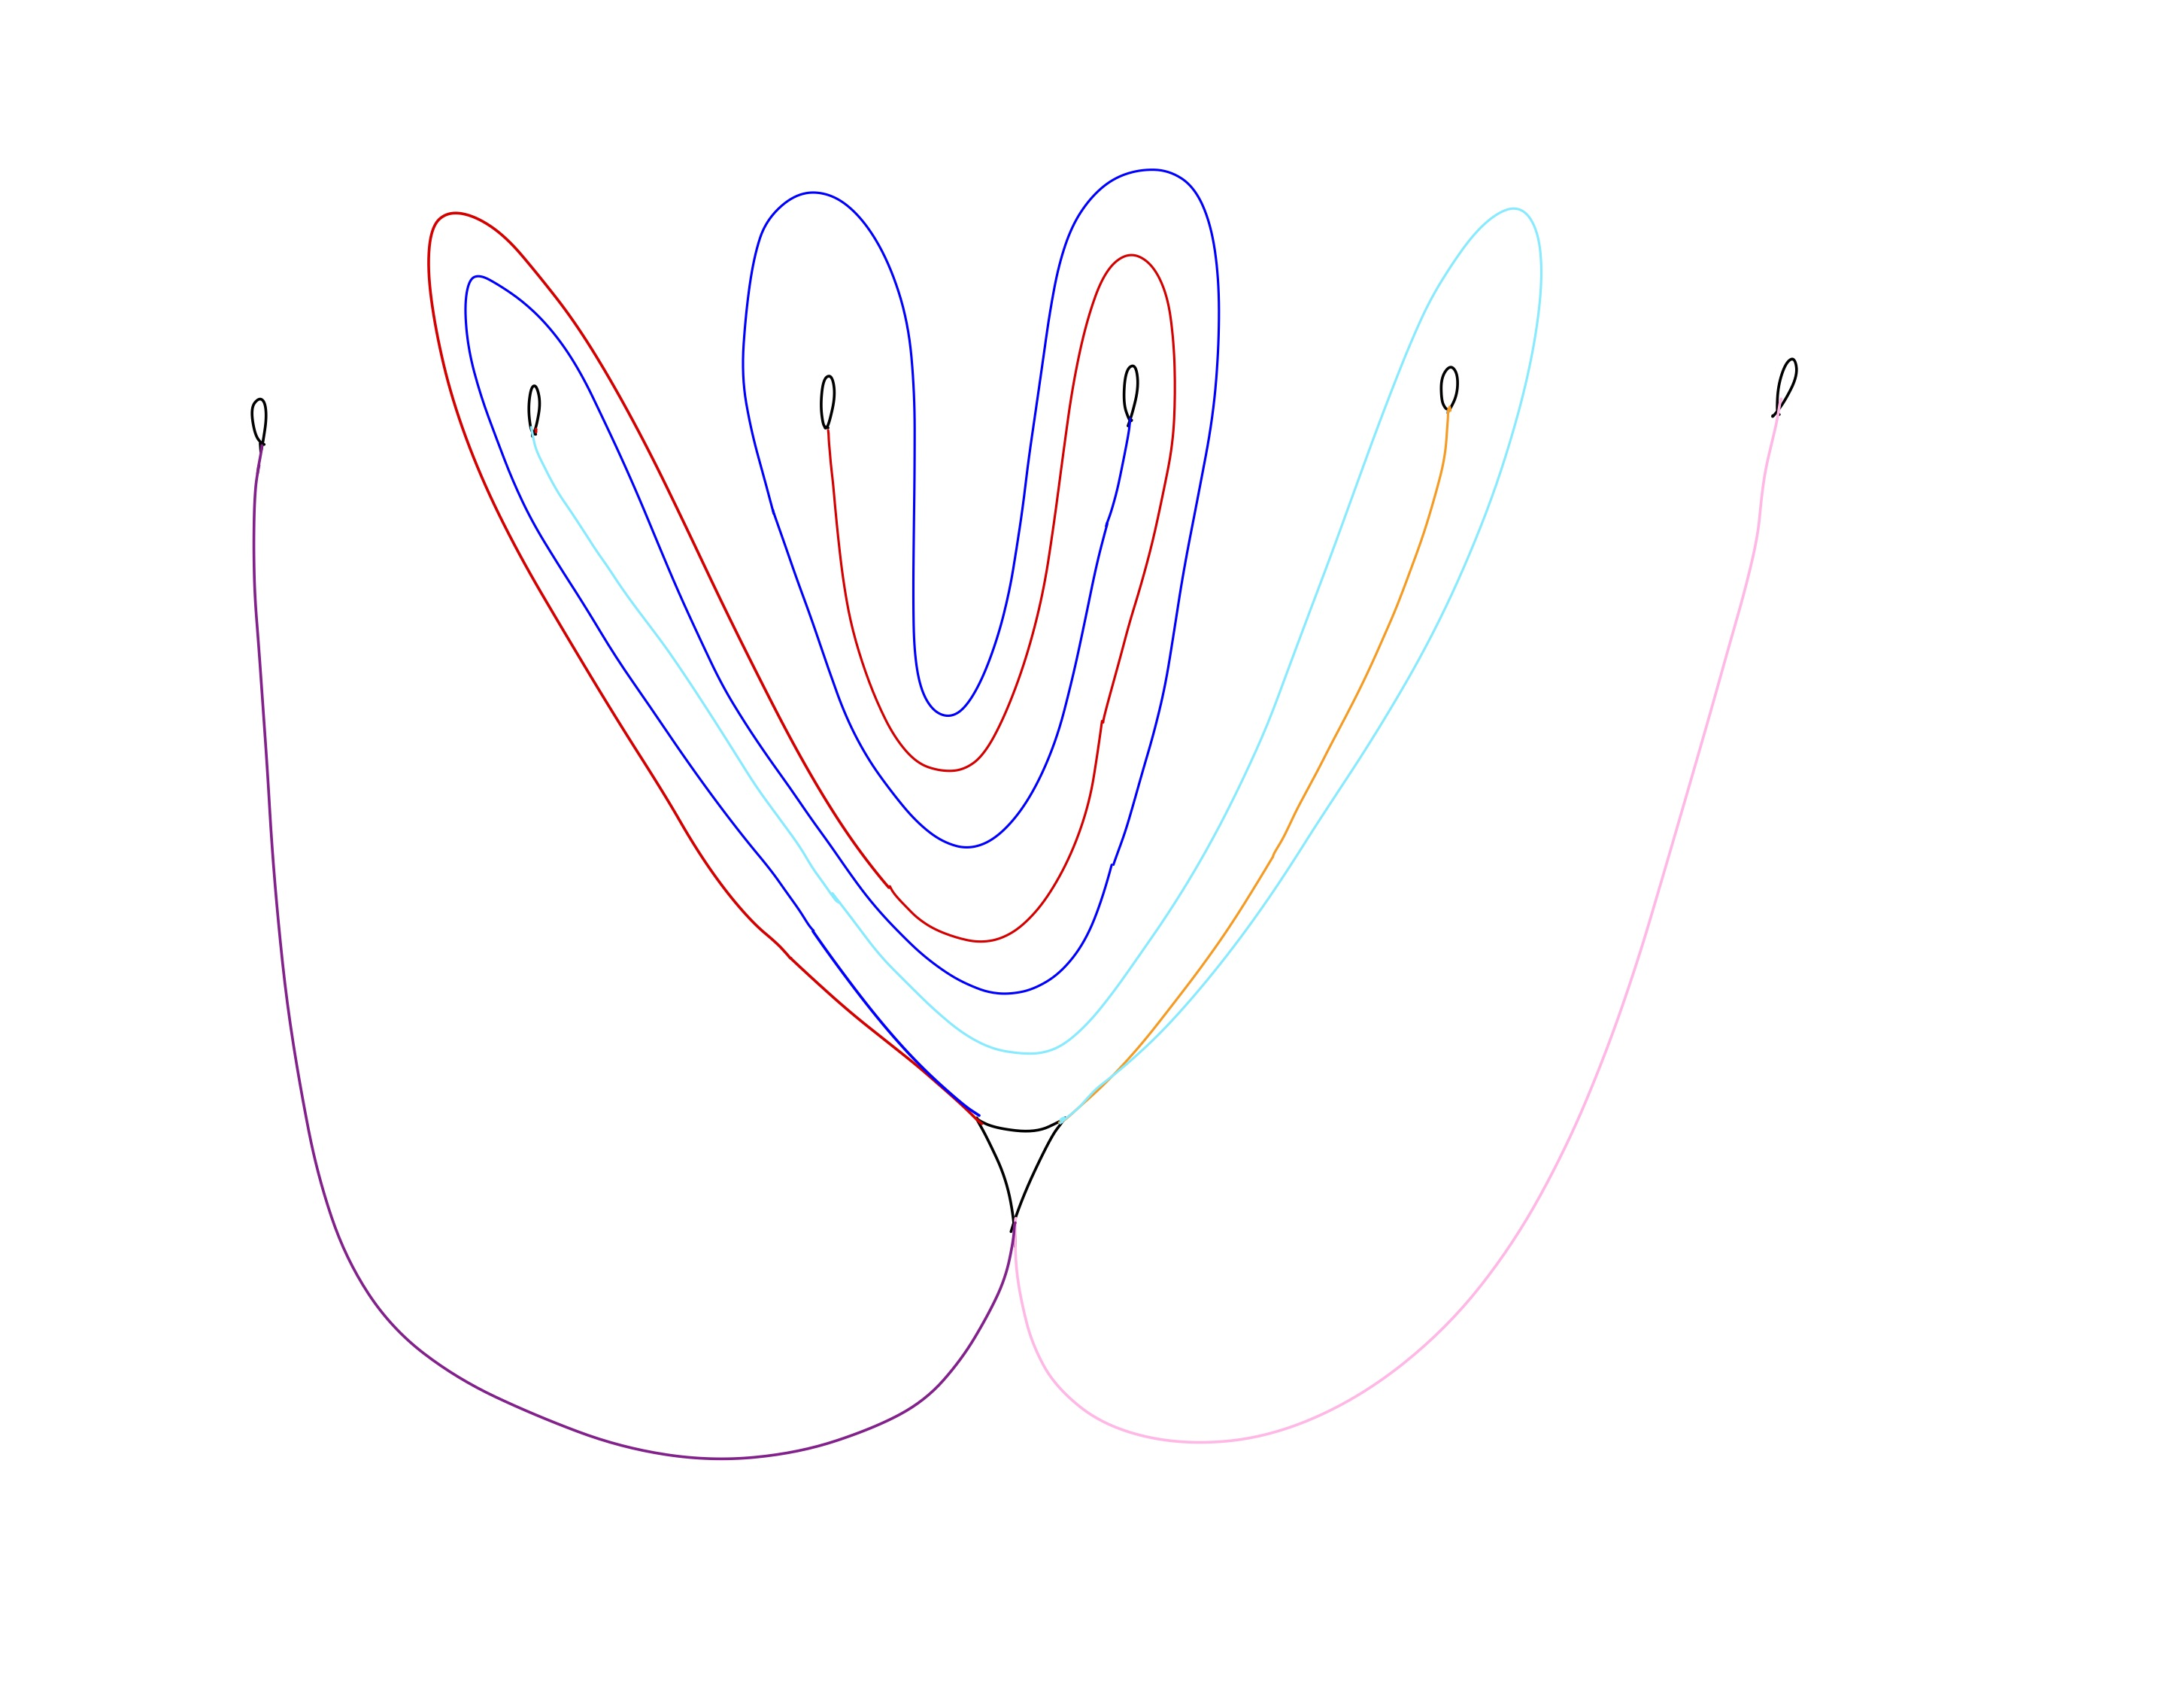
\includegraphics[width=\linewidth]{figures/Case Analysis Example Candelabra-13.jpg}
    \caption{The surviving family with one twist ($k = 1$) of $\fbb$ and $\fbr$ between $s$ and $i$ before termination.}
    \label{fig:Jehu_example_13}
\end{figure}

\begin{figure}[H]
    \centering
    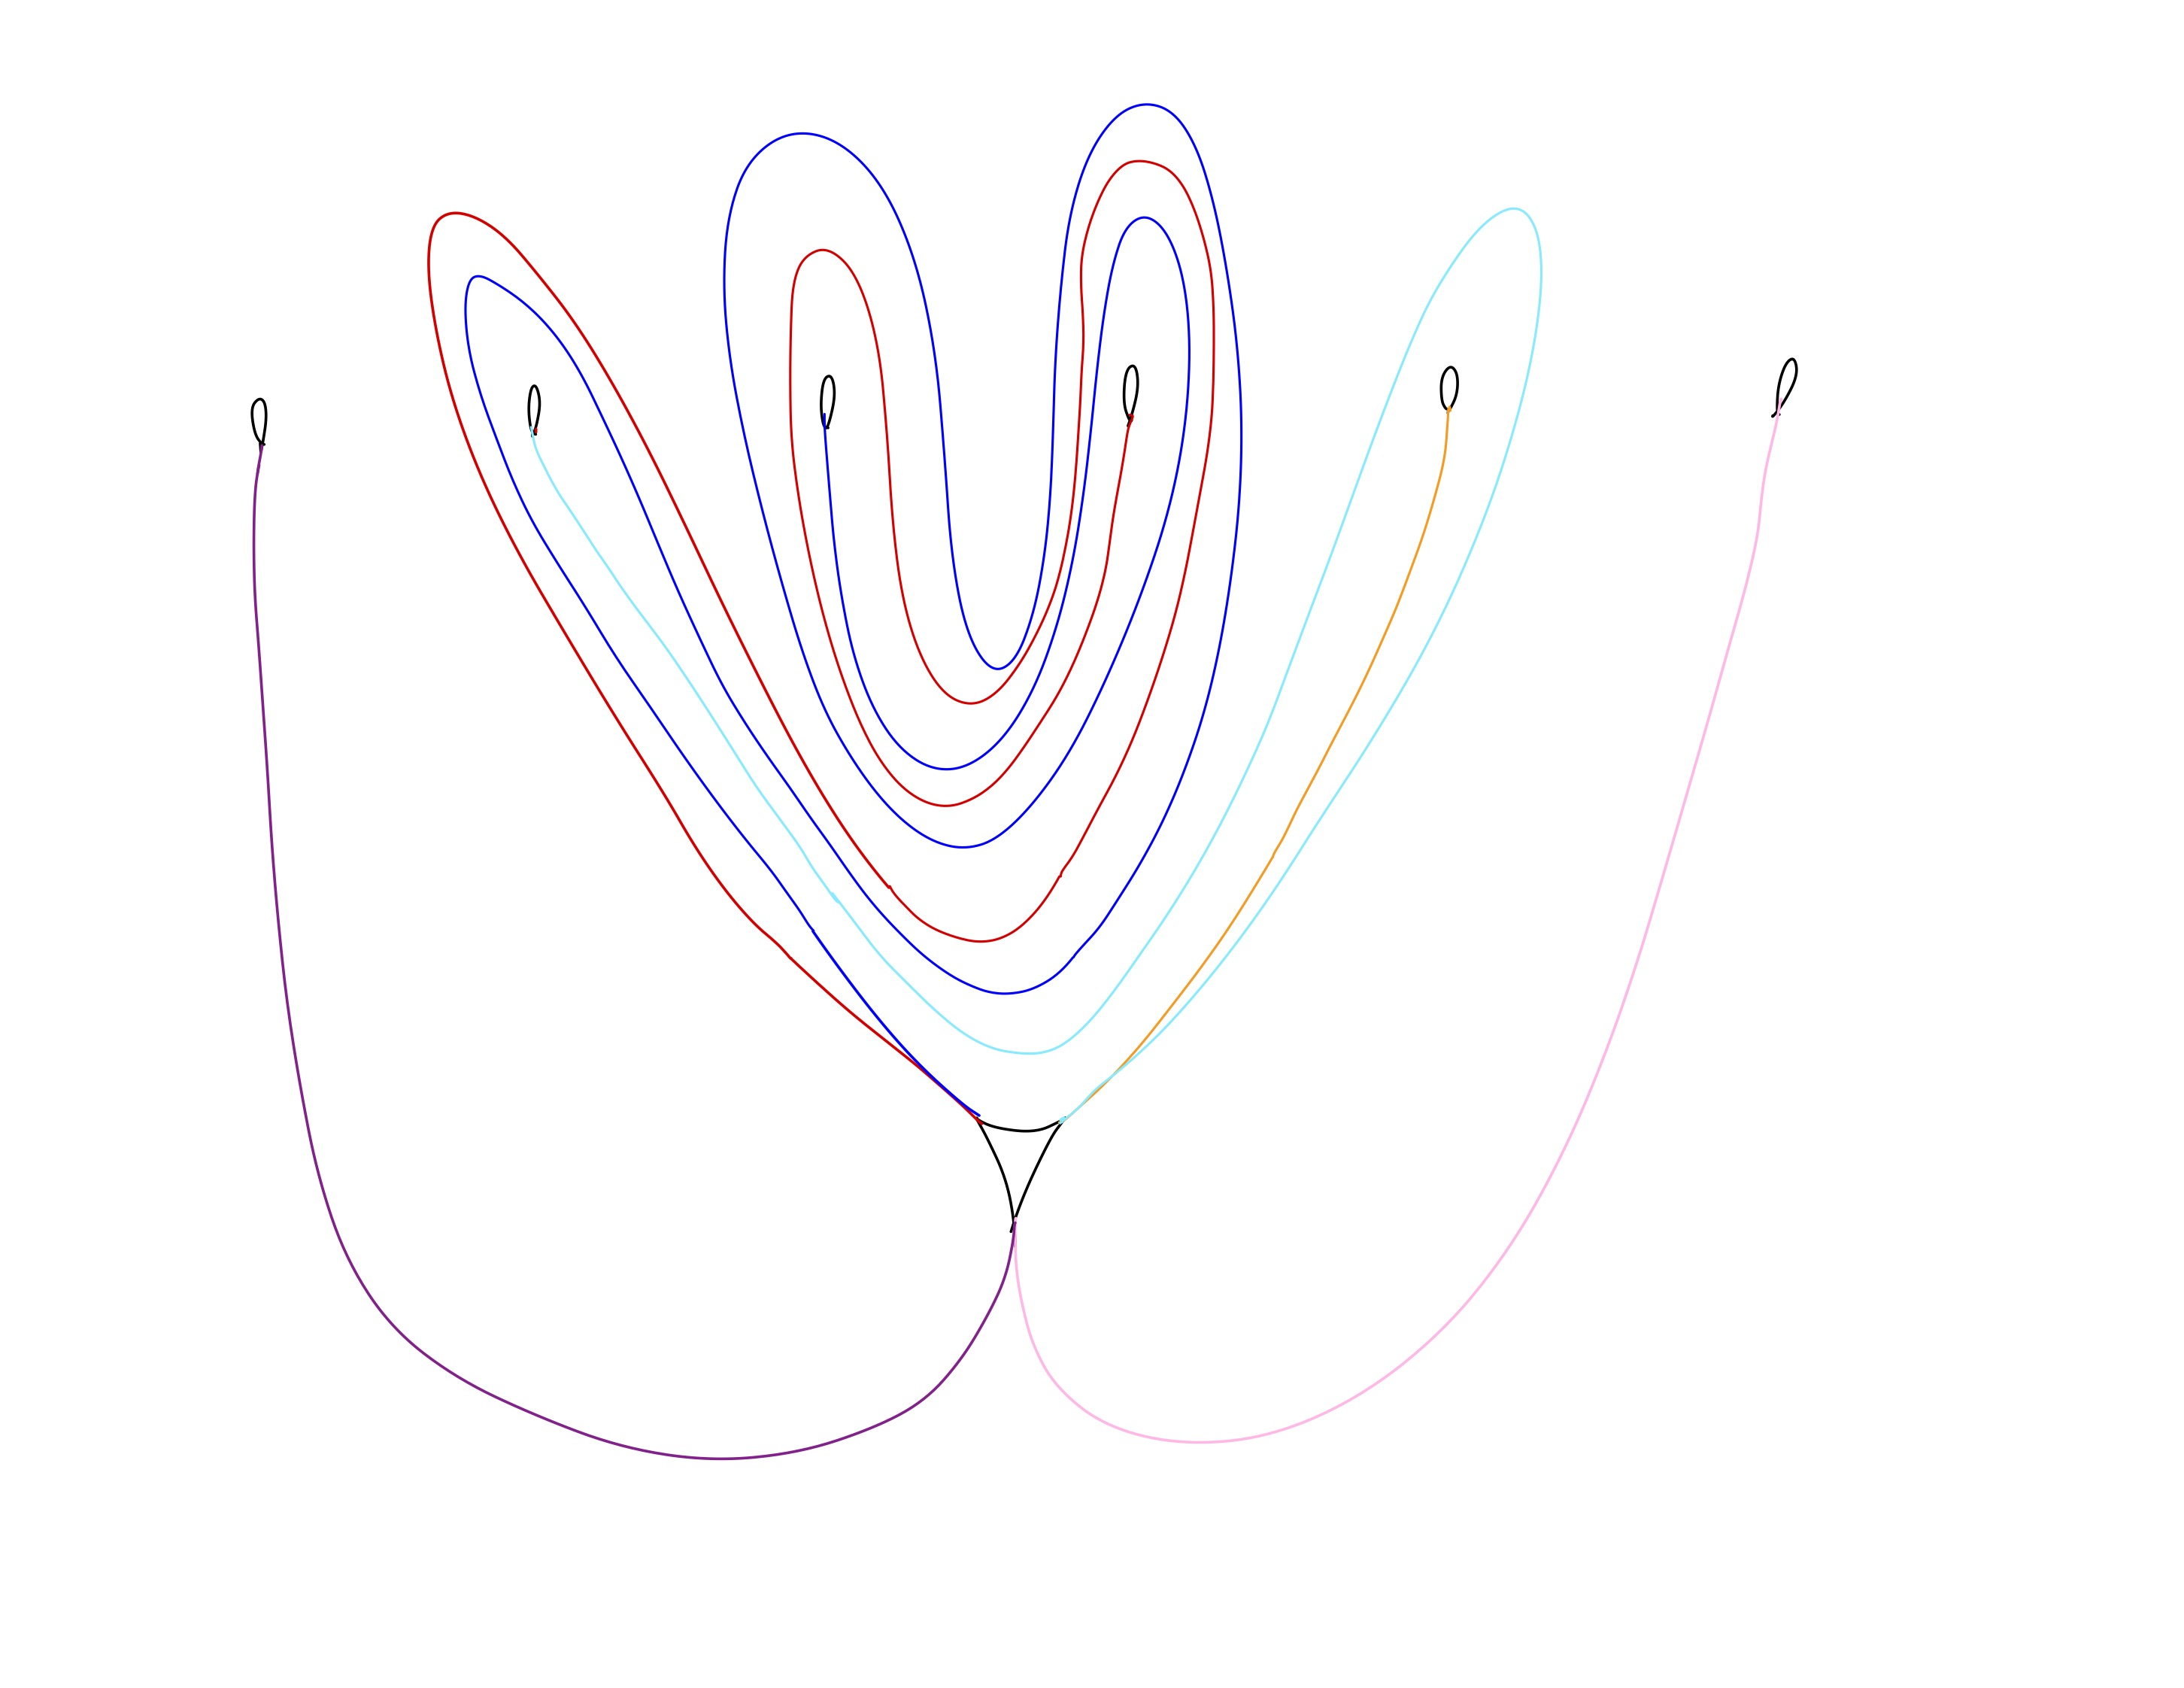
\includegraphics[width=\linewidth]{figures/Case Analysis Example Candelabra-14.jpg}
    \caption{The surviving family with two twists ($k = 2$). The general case admits an arbitrary $k \geq 0$ number of twists, with one of $\fbb, \fbr$ ending at $s^\circ$ and the other at $i^\circ$.}
    \label{fig:Jehu_example_14}
\end{figure}

\paragraph{Step 5--6 (Image paths and parameterization).} In conclusion, the resulting image paths are:
\begin{align*}
    f_\beta(p) &= b^\circ, \\
    f_\beta(o) &= p^\circ, \\
    f_\beta(i) &= r^\circ, \\
    f_\beta(s) &= p^+ o^\circ,
\end{align*}
together with the twisting pair $f_\beta(r)$ and $f_\beta(b)$, which twist between $s$ and $i$ an arbitrary $k \geq 0$ number of times, with one terminating at $s$ and the other at $i$. Precisely, we have either
\[
f_\beta(r) = o^- (i^+s^+)^k i^\circ \quad \text{and} \quad f_\beta(b) = o^- i^+ (s^+ i^+)^k s^\circ,
\]
or
\[
f_\beta(r) = o^- i^+ (s^+i^+)^k s^\circ \quad \text{and} \quad f_\beta(b) = o^- (i^+s^+)^k i^\circ.
\]
This family appears as Candidate Family 2 of the Candelabra train track in our full case analysis (Appendix \ref{app:case_analysis_candelabra}).

\paragraph{Step 7 (Braid extraction).} For each $k \geq 0$, this family is induced by a 6-braid of the form
\[
\beta = \Delta^{2i} (\sigma_3^k \cdot G_1 \cdot G_2)^{-1},
\]
where $i \in \mathbb{Z}$ is an arbitrary number of full twists (see Corollary \ref{cor:induce_by_braid_fulltwist}) and the two intermediate braid factors are
\begin{align*}
G_1 &= \sigma_2^{-1}\sigma_3^{-1}\sigma_4, \\
G_2 &= \sigma_{3}^{-1}\sigma_{4}^{-1}\sigma_{2}^{-1}\sigma_{3}^{-1}\sigma_{1}^{-1}\sigma_{2}^{-1}\sigma_{3}^{-1}\sigma_{4}^{-1}\sigma_{3}\sigma_{4}^{-1}\sigma_{5}^{-1}\sigma_{4}^{-1}\sigma_{3}^{-1}\sigma_{4}\sigma_{5}\sigma_{2}^{-1}\sigma_{1}^{-1}\sigma_{1}^{-1}\sigma_{2}^{-1}\sigma_{1}^{-1}\sigma_{1}^{-1} \\
&\quad \cdot \sigma_{5}\sigma_{4}\sigma_{3}\sigma_{2}\sigma_{1}\sigma_{2}\sigma_{3}\sigma_{4}\sigma_{5}\sigma_{5}\sigma_{4}\sigma_{3}\sigma_{2}\sigma_{3}\sigma_{4}\sigma_{5}\sigma_{5}\sigma_{4}\sigma_{3}\sigma_{4}\sigma_{5}\sigma_{5}\sigma_{4}\sigma_{5}\sigma_{5}.
\end{align*}
The derivation matches the stages described visually in Figure \ref{fig:candelabra_braid_b2} of Appendix \ref{app:candidate_braids_candelabra}: the factor $\sigma_3^k$ unwinds the $k$ twists between $\fbr$ and $\fbb$; the factor $G_1 = \sigma_2^{-1}\sigma_3^{-1}\sigma_4$ then transforms the unwound image to a standardized intermediate configuration; finally, $G_2$ transforms this intermediate back to the candelabra, as illustrated step by step in Figure \ref{fig:candelabra_braid_G}. The inverse of the product gives the candidate braid. We remind the reader that throughout this thesis, braid words are read from left to right.

By Corollary \ref{cor:induce_by_braid_fulltwist}, every 6-braid that induces this same family of train track maps differs from $\beta$ by a number of full twists. Up to conjugation, these braids represent candidates $\beta$ which can fit into the Birman-Hilden correspondence data.

\subsubsection*{Example 2: A Two-Triangle Track}
\label{subsec:example_two_triangles}

We now illustrate the procedure on a two-triangle track to demonstrate the additional features of Step 2 (the Cases A, B, C, D split) and Assumption A. We work on Track 0 (Figure \ref{fig:final_six_tracks}), one of the six irreducible jointless tracks in the stratum $(2;1^6;3^2)$. Track 0 has five real edges $b, i, o, p, r$ each incident to a jointless monogon, plus the central edge $d$ (and its symmetric companion $\bar{d}$) connecting the two infinitesimal triangles.

We focus on \emph{Case A} (triangles fixed). The analysis for Cases B, C, D proceeds analogously with odd parity replacing even at $d$-crossings.

\paragraph{Step 1 (Initial labeling).} The real edges $b, i, o, p, r$ are oriented toward their monogons; $d$ runs between the two triangles, with $\bar{d}$ its symmetric companion.

\paragraph{Step 2 (Triangle permutation).} We work in Case A: $f_\beta$ fixes the two infinitesimal triangles.

\paragraph{Step 3 (Initial letters under Assumption A).} The Trace Lemma applied to $b$, $i$, $o$, $p$, $r$ (each jointless-monogon-incident) forbids any of these edges from appearing in its own image path. For the central edge $d$, Assumption A requires that the first occurrence of $d$ in $f_\beta(d)$ be preceded by an even number of letters. Consider, for instance, an attempted start
\[
f_\beta(d) = r^+ d \ldots
\]
This places the first crossing of $d$ after a single letter ($r^+$), violating Assumption A. The same applies to any attempt to put $d$ in the second position of $f_\beta(d)$. The first $d$-crossing must therefore occur in an even position, so the start of $f_\beta(d)$ has the form
\[
f_\beta(d) = x^{\pm}\, y^{\pm}\, d \ldots
\]
or with more preceding letters (still in even count). The same parity constraint applies to $f_\beta(\bar{d})$.

\paragraph{Step 4 (Forced continuations).} Suppose we are exploring a branch in which
\[
f_\beta(d) = b^- p^- d \ldots, \qquad f_\beta(\bar{d}) = i^+ s^+ \bar{d} \ldots
\]
(Each begins with two letters preceding the central edge crossing, in agreement with Assumption A.) After the $d$-crossing in $f_\beta(d)$, the next letter is constrained by both the Trace Lemma and the Absorption Obstruction. The Trace Lemma requires that the next occurrence of $d$ in $f_\beta(d)$ be again preceded by an even number of letters since the previous $d$; equivalently, $d$ cannot reappear after a single letter. So a continuation of the form
\[
f_\beta(d) = b^- p^- d \cdot z^{\pm}\, d \ldots
\]
is forbidden, where $z^{\pm}$ is any single letter.

Independently, the Absorption Obstruction may forbid certain geometric routings of the continuation. Suppose the next letter is being chosen at a vertex where $f_\beta(i)$ and $f_\beta(o)$ have already established initial segments forming the cone $X_v(\fbi, \fbo)$. Then Lemma \ref{lem:cone_condition} forbids $f_\beta(d)$ from continuing into the interior of this cone:
\[
f_\beta(d) = b^- p^- d\, \Abso{\fbi}{\fbo} \ldots
\]
is invalid, and we record this with the absorption symbol $\times$.

\paragraph{Step 5 (Termination, contradictions, or survival).} Continuing the case analysis at each branching point eventually either:
\begin{enumerate}
    \item produces a complete candidate image word terminating with a $\circ$-decoration, or
    \item forces the dotted lines $f_\beta(d)$ and $f_\beta(\bar{d})$ to fail to join in the interior of the configuration. In the latter case, the dotted lines must continue around the outer perimeter of the train track, each successive $d$-crossing necessarily at an even position---but they continue indefinitely, never terminating. This is \emph{Situation $\alpha$}, and it produces a non-termination contradiction (Appendix \ref{app:case_analysis_preliminaries}).
\end{enumerate}
A third possibility is that the dotted lines do join in the interior but are forced into a region of the configuration from which they cannot escape without an odd-parity return to $d$. This is \emph{Situation $\beta$}, also called the bagged serpent.

\paragraph{Step 6 (Parameterization) and Step 7 (Braid extraction).} The surviving image paths organize into families parameterized by twist counts $k, m, j, \ldots$ between adjacent edges, exactly as in the candelabra example. For Track 0, the full case analysis (Appendix \ref{app:case_analysis_track0}) produces 13 such families, of which the family labeled \emph{Jubilant} provides one of the two F1-passing candidates in the homological filtering of Section \ref{sec:homological_filtering}. Each surviving family is then turned into an explicit candidate braid word by the same reverse-isotopy procedure used in Example 1.

\medskip

We do not attempt to walk through Track 0's complete case analysis here; the per-track appendix (Appendix \ref{app:case_analysis_track0}) is approximately 100 pages of step-by-step forced-letter reasoning across all four cases. The miniature derivation above shows the typical local move---enumerate next letters at each vertex, eliminate by the Trace Lemma or Absorption Obstruction, classify any failures as Situation $\alpha$, $\beta$, or path mill, and continue. For a worked instance of the resulting Jubilant family with concrete parameter values, see Figure \ref{fig:Jubilant3} of Appendix \ref{app:case_analysis_track0}.



%%%%%%%%%%%%%%%%%%%%%%%%%%%%%%%%%%%%%%%%%%%%%%%%%%%%%%%%%%%%%%%%%%%%%%%%
% HOMOLOGICAL FILTERING
%%%%%%%%%%%%%%%%%%%%%%%%%%%%%%%%%%%%%%%%%%%%%%%%%%%%%%%%%%%%%%%%%%%%%%%%

\section{Homological Filtering of Candidate Braids}
\label{sec:homological_filtering}

Once the topological constraints from Section \ref{sec:traintrack_analysis} isolate a finite list of candidate braid families $\beta \in B_6$ on the disk $D_6$ for a given stratum, we must determine which, if any, of these candidates can possibly correspond to the monodromy of a hyperbolic fibered knot $K$ satisfying $\widehat{HFK}(K) \cong \widehat{HFK}(T_{2,3}\# T_{2,3})$. To do this, we apply two filters, both of which are homological in nature. These tests utilize the Birman-Hilden correspondence to relate the action of the lifted braid to the topological invariants of the resulting knot complement.

Recall that our topological analysis determines the candidate braid only up to specific equivalences:
\begin{enumerate}
    \item \textbf{Conjugacy:} The combinatorial train track data identifies the conjugacy class of the braid, not a unique word.
    \item \textbf{Full Twists:} The mapping class is determined up to composition with powers of the full twist $\Delta^2$ (the generator of the center of $B_6$, corresponding to a Dehn twist along the boundary of the disk).
    \item \textbf{Chirality (Mirroring):} The analysis deliberately does not distinguish between $\beta$ and its mirror image $\beta^{-1}$.
\end{enumerate}

Under the Birman-Hilden correspondence, these braids lift to a diffeomorphism $\Phi$ on the double branched cover $\Sigma_2^2$. We will explicitly derive the action of this lift on the homology of the surface and compute the characteristic polynomial of the induced map. Crucially, this filtering process is well-defined on the equivalence classes described above. As we will formally establish, the characteristic polynomial is invariant under matrix conjugation, the full twist lifts to the identity map on the relevant homology group, and the symplectic nature of the action ensures that mirroring leaves the polynomial unchanged. Consequently, it suffices to test a single representative braid word for each candidate family.

\subsection{The Action on Homology}

A candidate braid $\beta$ lifts to a diffeomorphism $\Phi$ on the double cover of the disk branched over the six marked points. This cover is a genus-2 surface with two boundary components, denoted $\Sigma_2^2$. The map $\Phi \colon \Sigma_2^2 \to \Sigma_2^2$ induces a linear action on the first homology:
\[
\Phi_* \colon H_1(\Sigma_2^2; \mathbb{Z}) \to H_1(\Sigma_2^2; \mathbb{Z}).
\]

The first homology group $H_1(\Sigma_2^2; \mathbb{Z})$ has rank 5 and splits as $V \oplus \partial V$, where $V \cong \mathbb{Z}^4$ is the symplectic subspace generated by the handles of the surface, and $\partial V$ is the subspace generated by the boundary cycles $\partial_1, \partial_2$ (modulo the relation $\partial_1 + \partial_2 = 0$).

To compute the homological action, we translate the braid generators on the disk into matrices. Each standard braid generator $\sigma_i$ on $D_6$ swaps two adjacent marked points via a half-twist. In the double branched cover, the preimage of the arc connecting these points is a simple closed curve $\gamma_i$. The lift of the half-twist is a full Dehn twist $T_{\gamma_i}$ along this curve. Because the standard braid generators are supported entirely in the interior of the disk, their lifts are supported in the interior of $\Sigma_2^2$, meaning they fix the boundary components pointwise.

Since the action acts as the identity on $\partial V$, the matrix representation of $\Phi_*$ with respect to a basis adapted to the decomposition $V \oplus \mathbb{Z}\langle \partial_1 \rangle$ takes the block upper-triangular form:
\[
\Phi_* = \begin{pmatrix}
A_{\text{red}} & * \\
0 & 1
\end{pmatrix}.
\]
We define the \emph{reduced action} $A_{\text{red}}$ as the map induced on the quotient space:
\[
H_1(\Sigma_2^2) / \langle \partial_1, \partial_2 \rangle \cong H_1(\Sigma_2; \mathbb{Z}).
\]
Geometrically, this corresponds to ``capping off'' both boundary components with disks to obtain the closed genus-2 surface $\Sigma_2$, and computing the action on the homology of this closed manifold.

\subsubsection{Explicit Matrix Representation}

We identify the reduced homology $H_1(\Sigma_2; \mathbb{Z})$ with the standard lattice $\mathbb{Z}^4$ by fixing a symplectic basis $\mathcal{B} = \{e_1, e_2, e_3, e_4\}$. Geometrically, this basis corresponds to the standard system of curves on the genus-2 surface, where $e_1, e_3$ represent the meridians ($a$-cycles) and $e_2, e_4$ represent the dual longitudes ($b$-cycles) of the two handles. These elements satisfy the standard algebraic intersection relations:
\[
\langle e_1, e_2 \rangle = \langle e_3, e_4 \rangle = 1, \quad \text{and} \quad \langle e_i, e_j \rangle = 0 \text{ otherwise.}
\]

The action of a Dehn twist $T_{\gamma_i}$ on a homology class $x$ is given by the Picard-Lefschetz formula:
\begin{equation}
    T_{\gamma_i}(x) = x + \langle x, [\gamma_i] \rangle [\gamma_i].
\end{equation}
By applying this formula to each basis vector $e_j$, we derive the explicit symplectic matrices $M_i \in \text{Sp}(4, \mathbb{Z})$ representing the action of the lifted generators $\sigma_i$ on the closed surface $\Sigma_2$:

\begin{align}
M_1 &= \begin{pmatrix} 1 & -1 & 0 & 0 \\ 0 & 1 & 0 & 0 \\ 0 & 0 & 1 & 0 \\ 0 & 0 & 0 & 1 \end{pmatrix}, &
M_2 &= \begin{pmatrix} 1 & 0 & 0 & 0 \\ 1 & 1 & -1 & 0 \\ 0 & 0 & 1 & 0 \\ 0 & 0 & 0 & 1 \end{pmatrix}, \\
M_3 &= \begin{pmatrix} 1 & 0 & 0 & 0 \\ 0 & 1 & 0 & 0 \\ 0 & 1 & 1 & -1 \\ 0 & 0 & 0 & 1 \end{pmatrix}, &
M_4 &= \begin{pmatrix} 1 & 0 & 0 & 0 \\ 0 & 1 & 0 & 0 \\ 0 & 0 & 1 & 0 \\ 0 & 0 & 1 & 1 \end{pmatrix}, \\
M_5 &= \begin{pmatrix} 1 & 0 & 0 & -1 \\ 0 & 1 & 0 & 0 \\ 0 & 0 & 1 & -1 \\ 0 & 0 & 0 & 1 \end{pmatrix}.
\end{align}

For any representative braid word $\beta = \sigma_{i_1}^{k_1} \dots \sigma_{i_m}^{k_m}$, the action on the reduced homology is given exactly by the matrix product:
\begin{equation}
    A_{\text{red}} = \prod_{j=1}^m M_{i_j}^{k_j}.
\end{equation}

\subsection{Invariance Properties of the Filter}

The filtering process using the characteristic polynomial of $A_{\text{red}}$ is well-defined on the equivalence classes of our candidate braids:
\begin{itemize}
    \item \textbf{Conjugacy:} The characteristic polynomial is a similarity invariant, meaning conjugate braids yield identical polynomials.
    \item \textbf{Full Twists:} The central element $\Delta^2$ corresponds to a Dehn twist along the boundary of $D_6$. Upon lifting and capping to $\Sigma_2$, this becomes a Dehn twist along a trivial curve (bounding a disk), which is isotopic to the identity. Algebraically, the half-twist $\Delta$ lifts to the hyperelliptic involution $\iota$, which acts as $-I$ on $H_1(\Sigma_2; \mathbb{Z})$. Consequently, the full twist $\Delta^2$ acts as $(-I)^2 = I$. Thus, $A_{\text{red}}$ is invariant under the addition of full twists.
    \item \textbf{Mirroring:} Mirroring $\beta$ (replacing each $\sigma_i$ with $\sigma_i^{-1}$) replaces $A_{\text{red}}$ with $A_{\text{red}}^{-1}$. Since $A_{\text{red}}$ is a symplectic matrix, its characteristic polynomial is reciprocal, meaning $P(t) = t^4 P(t^{-1})$. Consequently, the characteristic polynomials of $A_{\text{red}}$ and $A_{\text{red}}^{-1}$ are identical. The filter is insensitive to chirality.
\end{itemize}

\subsection{Verification via Zero-Surgery}
\label{subsec:zero_surgery_check}

The first filter verifies that the candidate braid produces a knot embedded in the correct ambient manifold, specifically the 3-sphere $S^3$.

Let $Y$ be the 3-manifold associated with the open book decomposition defined by the page $\Sigma_2^2$ and the lifted monodromy $\Phi$. The binding of this open book is a two-component link $L = L_1 \cup L_2$, corresponding to the two boundary components of the surface. We identify one component, say $L_1$, as the candidate for the knot $K$.

Topologically, capping off the boundary component corresponding to $L_2$ is equivalent to performing zero-surgery on $L_2$. This operation yields a new manifold $Y'$ containing the single knot $L_1$. For $L_1$ to be a valid candidate for the knot $K \subset S^3$, the ambient manifold $Y'$ must be an integer homology sphere (such that $H_1(Y'; \mathbb{Z}) = 0$).

Using the exact sequence for the mapping torus, the order of the first homology is determined by the determinant of $(I - h_*)$, where $h_*$ is the monodromy acting on the fiber. In our reduced basis, this condition dictates that for $Y'$ to be a homology sphere, we require:
\begin{equation}\label{eq:homology_check_det_equal_1}
    |\det(I - A_{\text{red}})| = 1.
\end{equation}
If this determinant evaluates to anything other than $\pm 1$, the resulting manifold $Y'$ possesses non-trivial torsion (e.g., it may be a Lens space), which implies the knot $L_1$ cannot reside in $S^3$. Any candidate braid family failing this condition is immediately eliminated.

\subsection{Verification via the Alexander Polynomial}
\label{subsec:alexander_poly_check}

The second, finer filter compares the induced characteristic polynomial of the surviving candidates to that of the target knot. The Alexander polynomial $\Delta_K(t)$ is the characteristic polynomial of the monodromy acting on the symplectic homology of the fiber. For $K = T_{2,3} \# T_{2,3}$, this is exactly:
\[
\Delta_K(t) = (t^2 - t + 1)^2.
\]

A technical subtlety arises because the candidate braids are defined on the disk (lifting to the surface with boundary $\Sigma_2^2$), while the standard Alexander polynomial is an invariant of the closed fiber. We rely on the following lemma to justify comparing the polynomial computed from our reduced matrices $M_i$ directly to $\Delta_K(t)$.

\begin{lemma}
\label{lem:capping_invariance}
Let $f \colon \Sigma_g^n \to \Sigma_g^n$ be a homeomorphism that preserves the boundary components pointwise. Let $A$ be the matrix of $f_*$ on $H_1(\Sigma_g^n; \mathbb{Z})$ and $A_{\text{red}}$ be the matrix of the induced map on the capped closed surface $\Sigma_g$. Then:
\[
\det(tI - A) = (t-1)^n \det(tI - A_{\text{red}}).
\]
\end{lemma}

\begin{proof}
We decompose the first homology group $H_1(\Sigma_g^n; \mathbb{Z})$ as $V \oplus \partial V$, where $V \cong H_1(\Sigma_g; \mathbb{Z}) \cong \mathbb{Z}^{2g}$ is the symplectic subspace generated by the handles, and $\partial V \cong \mathbb{Z}^n$ is the subspace generated by the boundary cycles. Since $f$ fixes the boundary components pointwise, the induced map $f_*$ acts as the identity on $\partial V$. Furthermore, since $f$ preserves the boundary, it maps the subspace $V$ into $V \oplus \partial V$. With respect to a basis reflecting this decomposition, the matrix $A$ representing $f_*$ takes the block upper-triangular form:
\[
A = \begin{pmatrix}
A_{\text{red}} & * \\
0 & I_n
\end{pmatrix},
\]
where $A_{\text{red}}$ is the matrix of the map induced on the quotient $H_1(\Sigma_g^n) / \partial V \cong H_1(\Sigma_g)$, and $I_n$ is the $n \times n$ identity matrix. Because the characteristic polynomial of a block triangular matrix is the product of the characteristic polynomials of its diagonal blocks, we obtain:
\[
\det(tI - A) = \det(tI - A_{\text{red}}) \cdot \det(tI - I_n) = \det(tI - A_{\text{red}}) \cdot (t-1)^n.
\]
\end{proof}

\begin{remark}
Geometrically, capping a boundary is equivalent to trivializing the homology cycle corresponding to that boundary loop. Before capping, these trivial actions manifest as factors of $(t-1)$ in the characteristic polynomial because the boundary components are strictly fixed by the monodromy.
\end{remark}

Since we have explicitly computed $A_{\text{red}}$ using the matrices $M_i$ (which correspond to the action on the closed surface), we have effectively removed the boundary artifacts described in Lemma \ref{lem:capping_invariance}. Therefore, the characteristic polynomial must match the standard Alexander polynomial $\Delta_K(t)$ exactly, without any additional factors of $(t-1)$. We verify if:
\begin{equation}
    \det(tI - A_{\text{red}}) = (t^2 - t + 1)^2.
\end{equation}
Any candidate braid failing this exact equality is eliminated, concluding our obstruction.


%%%%%%%%%%%%%%%%%%%%%%%%%%%%%%%%%%%%%%%%%%%%%%%%%%%%%%%%%%%%%%%%%%%%%%%%
% SKELETON: STRATUM (3;1^6;3)
%%%%%%%%%%%%%%%%%%%%%%%%%%%%%%%%%%%%%%%%%%%%%%%%%%%%%%%%%%%%%%%%%%%%%%%%

\section{The Stratum \texorpdfstring{$(3;1^6;3)$}{(3;1\textasciicircum 6;3)}}
\label{sec:analysis_3_16_3}

We now apply our geometric and algebraic machinery to the first of the two non-orientable strata. Our ultimate goal for this section is to rigorously establish the following elimination theorem:

\begin{theorem}\label{thm:candelabra_stratum_classification}
    Let $K \subset S^3$ be a hyperbolic knot satisfying $\widehat{HFK}(K) \cong \widehat{HFK}(T_{2,3} \# T_{2,3})$, and let
    \[
    (h, \phi_h, \hat{h}, \hat{\phi}_h, b, \phi_b, \beta, \phi_\beta, \Phi, \phi_\Phi)
    \]
    be the associated Birman-Hilden correspondence data induced by the monodromy of $K$. Then the pseudo-Anosov 6-braid $\beta$ on the disk cannot belong to the stratum $(3;1^6;3)$.
\end{theorem}

To prove this theorem, we must traverse the full obstruction pipeline: generating the state space, pruning it via tight splitting, enumerating the valid mapping classes, and applying homological filters.

\subsection{Reducing Candidate Train Tracks via Splitting}

We begin by demonstrating that any pseudo-Anosov map in this stratum must be carried by a single specific train track.

\begin{lemma}\label{lem:candelabra_reduction}
    Let $\beta$ be a pseudo-Anosov 6-braid in the stratum $(3;1^6;3)$ that lifts to a fixed-point-free mapping class on $\Sigma_2^2$. If $\beta$ is carried by a standard train track $\tau$, then up to conjugation and mirroring, $\tau$ is the Candelabra train track (Figure \ref{fig:candelabra}).
\end{lemma}

\begin{proof}
    Running the \texttt{autofolder} algorithm on the stratum $(3;1^6;3)$ yields an exhaustive train track automaton configured as a directed graph with 138 vertices and 706 directed edges. Among these 138 standard train tracks, there are exactly 4 which are jointless. These are shown in Figure \ref{fig:candelabra_stratum}. By Corollary \ref{cor:jointless_track}, up to conjugation, we only need to consider these four tracks.

    \begin{figure}[ht]
        \centering
        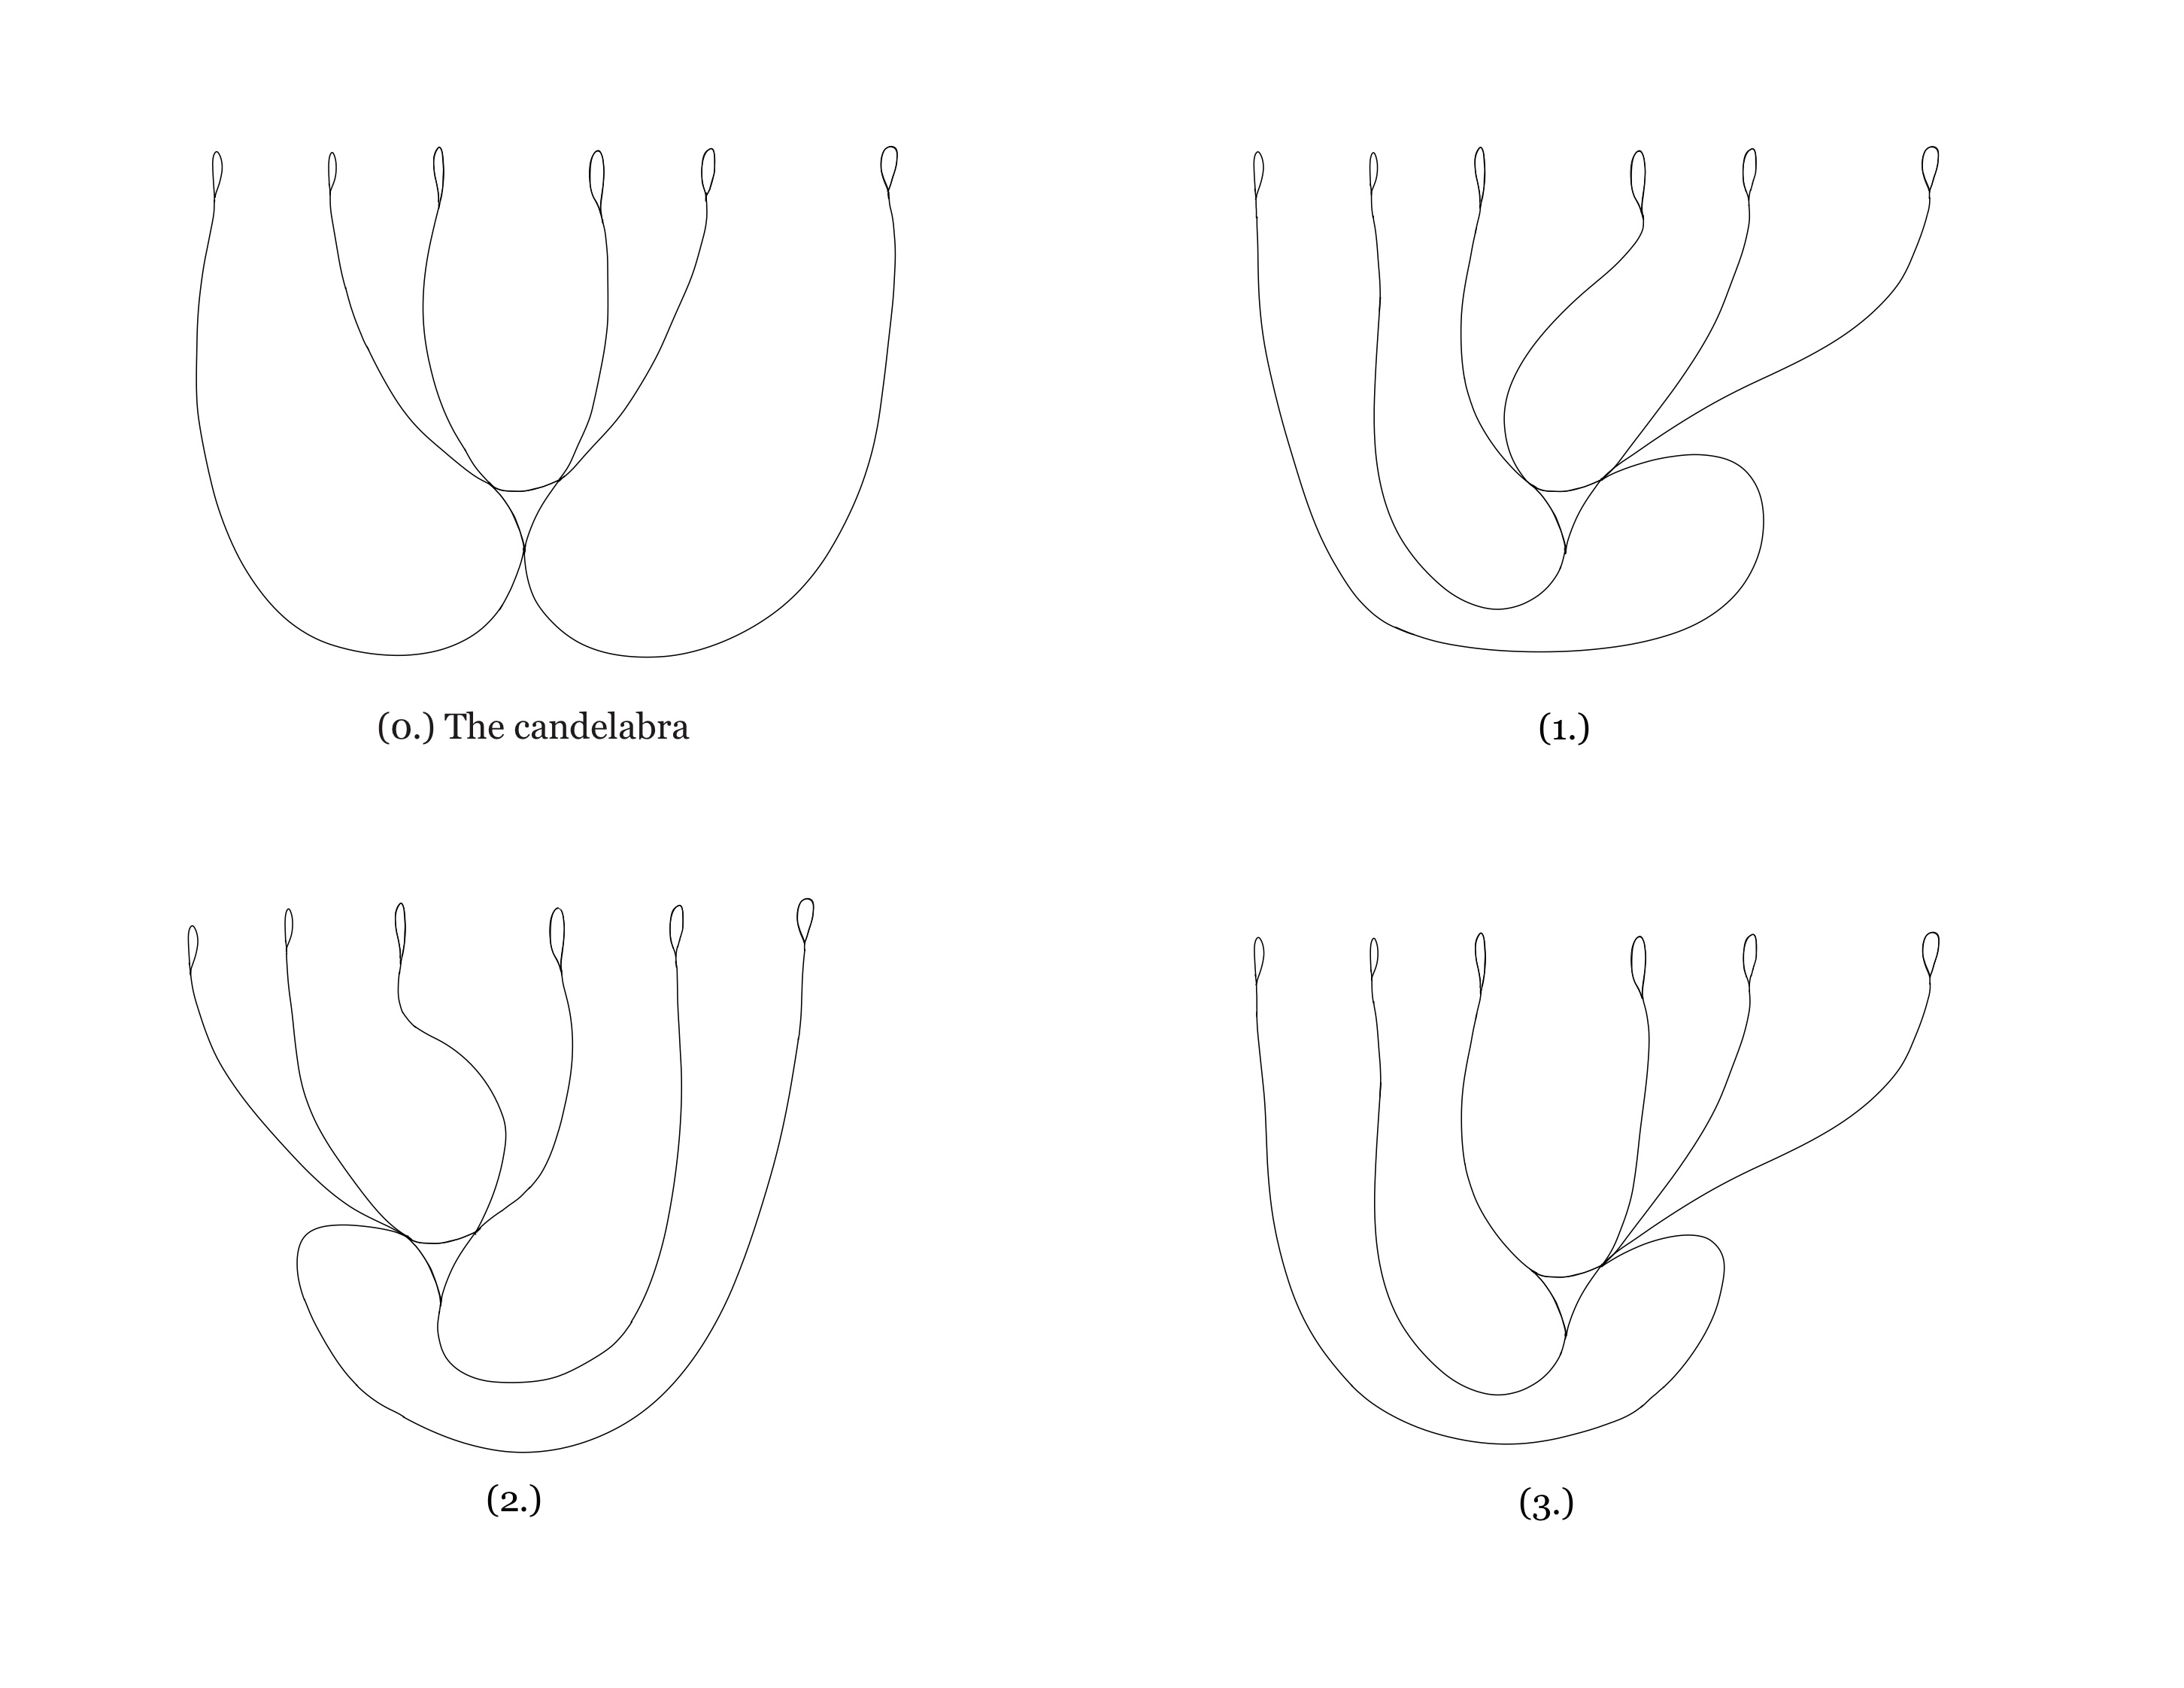
\includegraphics[width=\linewidth]{figures/Candelabra_stratum-5.jpg}
        \caption{The four jointless standard train tracks in the stratum $(3;1^6;3)$. Track 0 is the Candelabra.}
        \label{fig:candelabra_stratum}
    \end{figure}

    We construct splitting diagrams for these candidate tracks. Figure \ref{fig:candelabra_splitting_3} shows that Train Track 3 eventually splits to Train Track 1 or 2. Figure \ref{fig:candelabra_splitting_1} shows that Train Track 1 eventually splits to the Candelabra (Track 0), or Train Track 2.

    \begin{figure}[ht]
        \centering
        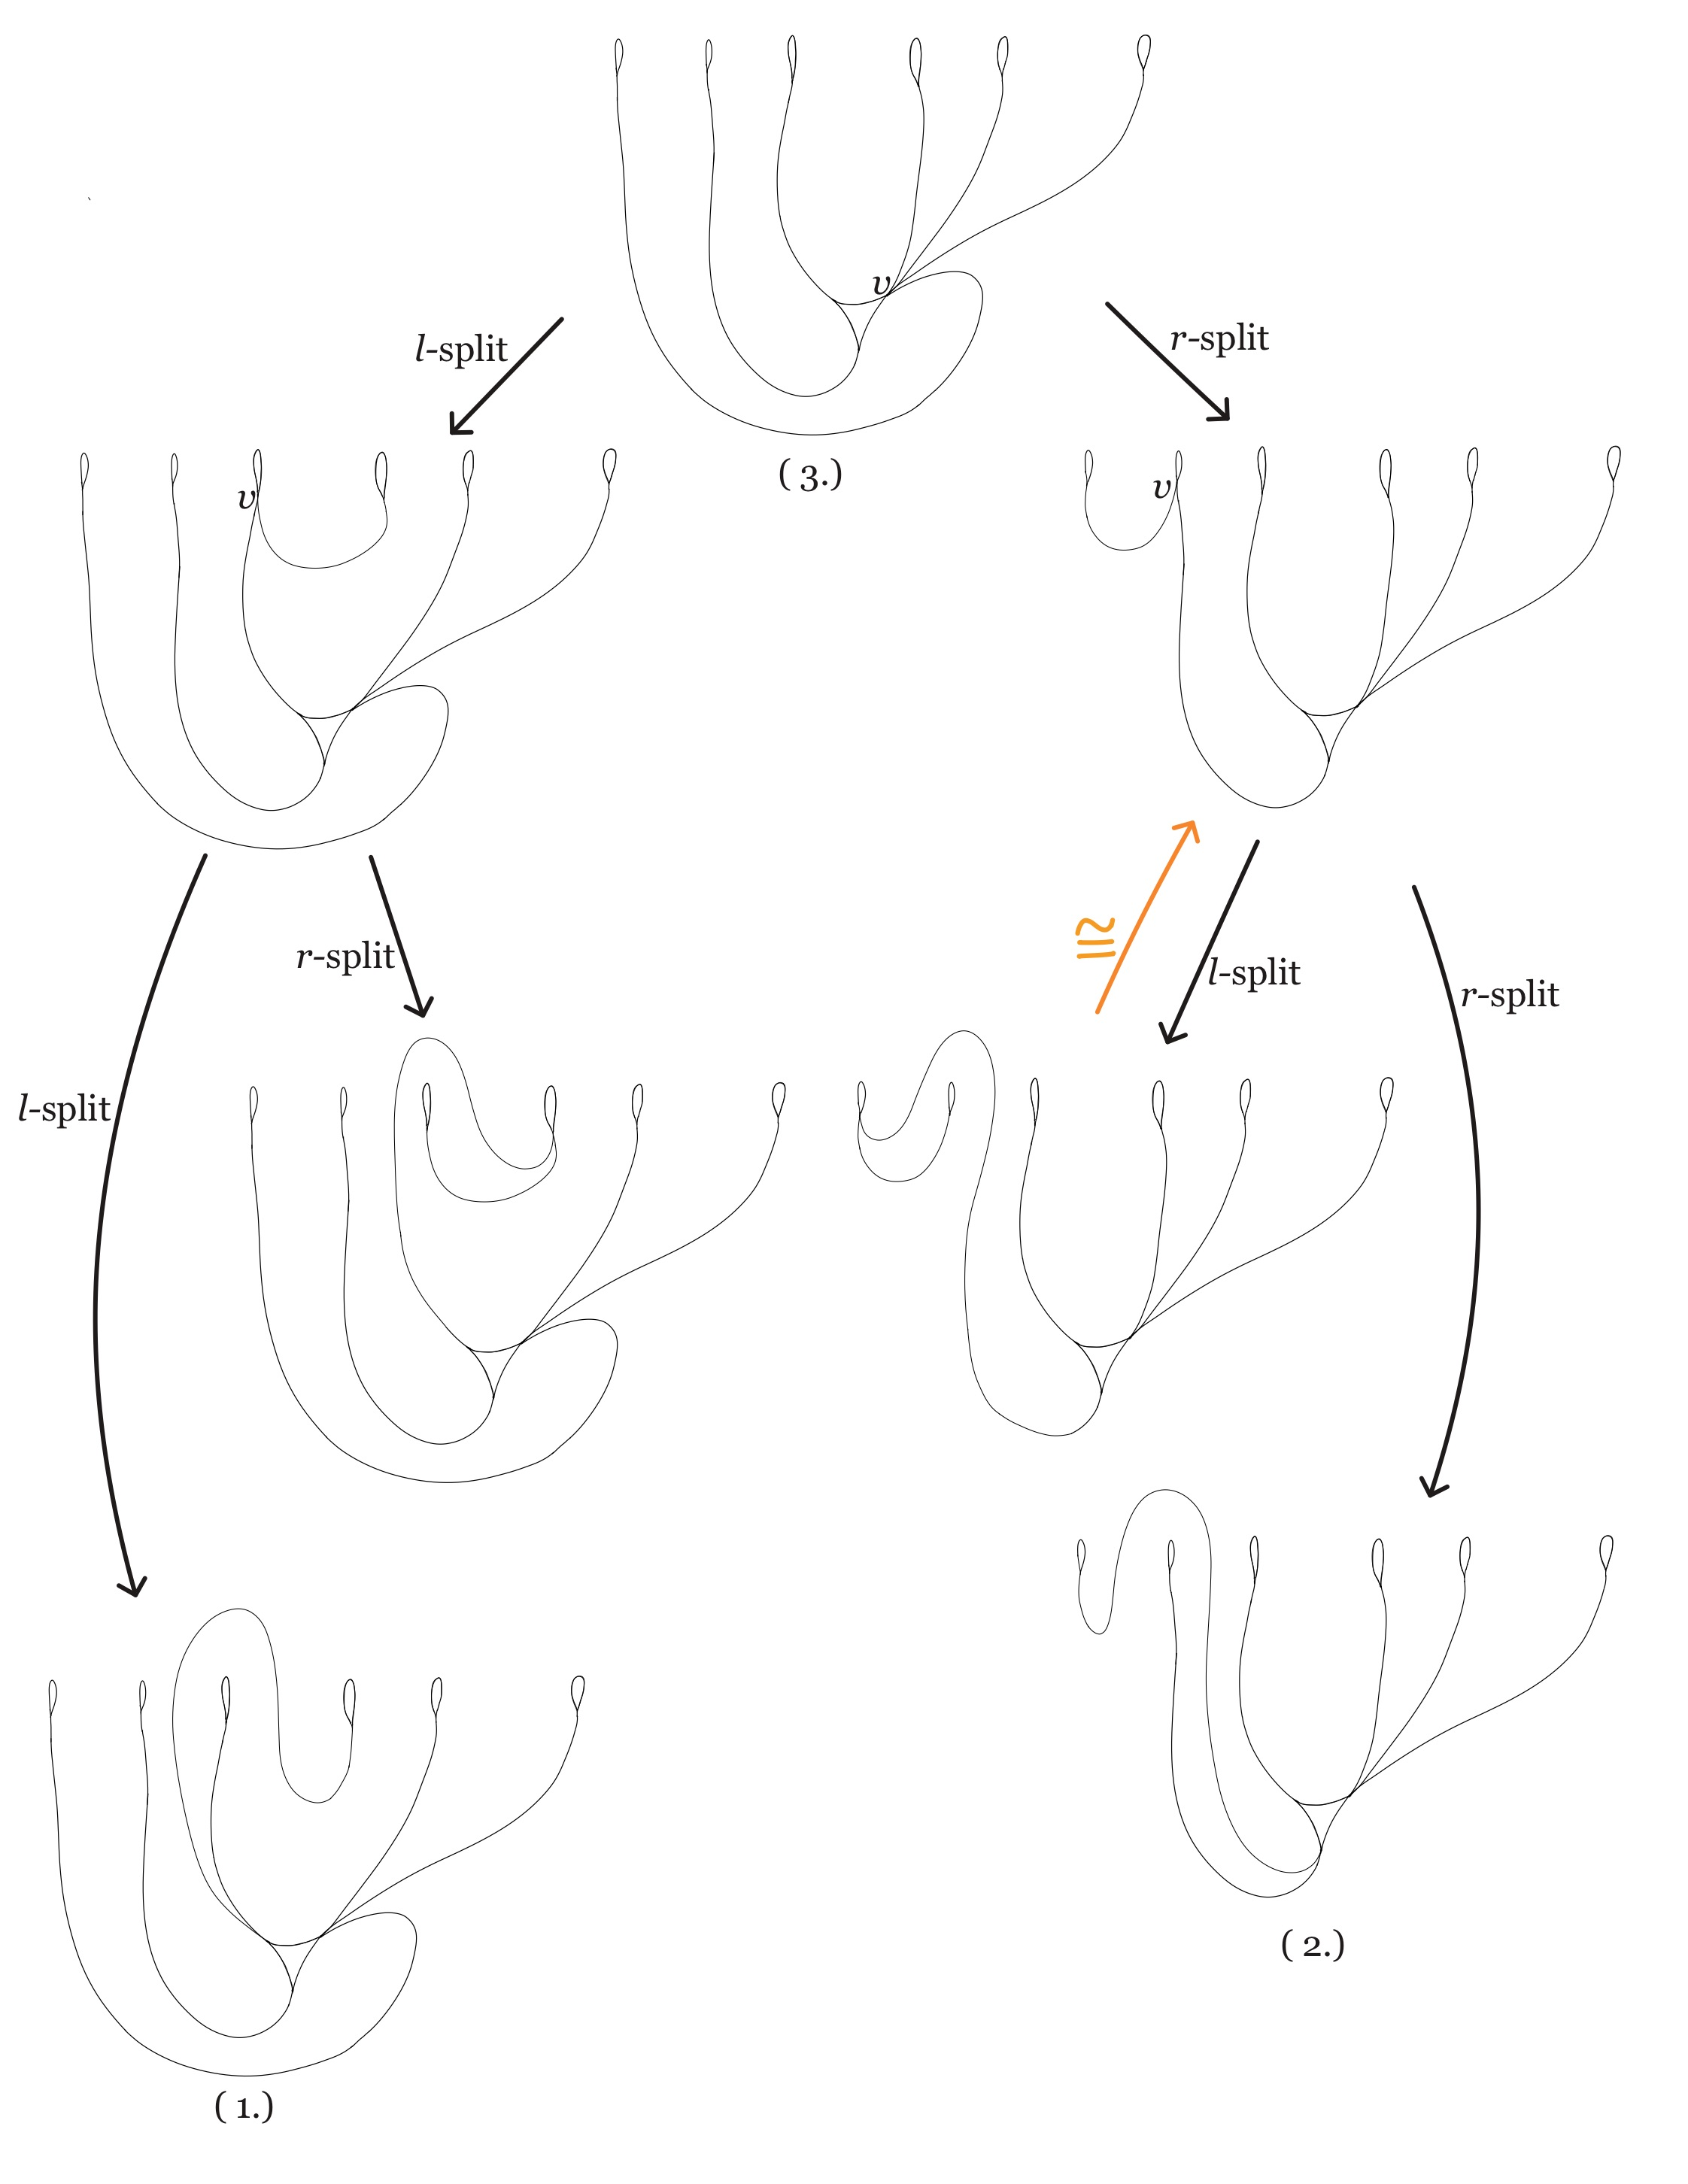
\includegraphics[width=\linewidth]{figures_splitting/Candelabra Splitting 3-5.jpg}
        \caption{Train Track 3 eventually splits to Train Track 1 or the Candelabra.}
        \label{fig:candelabra_splitting_3}
    \end{figure}

    \begin{figure}[p]
        \centering
        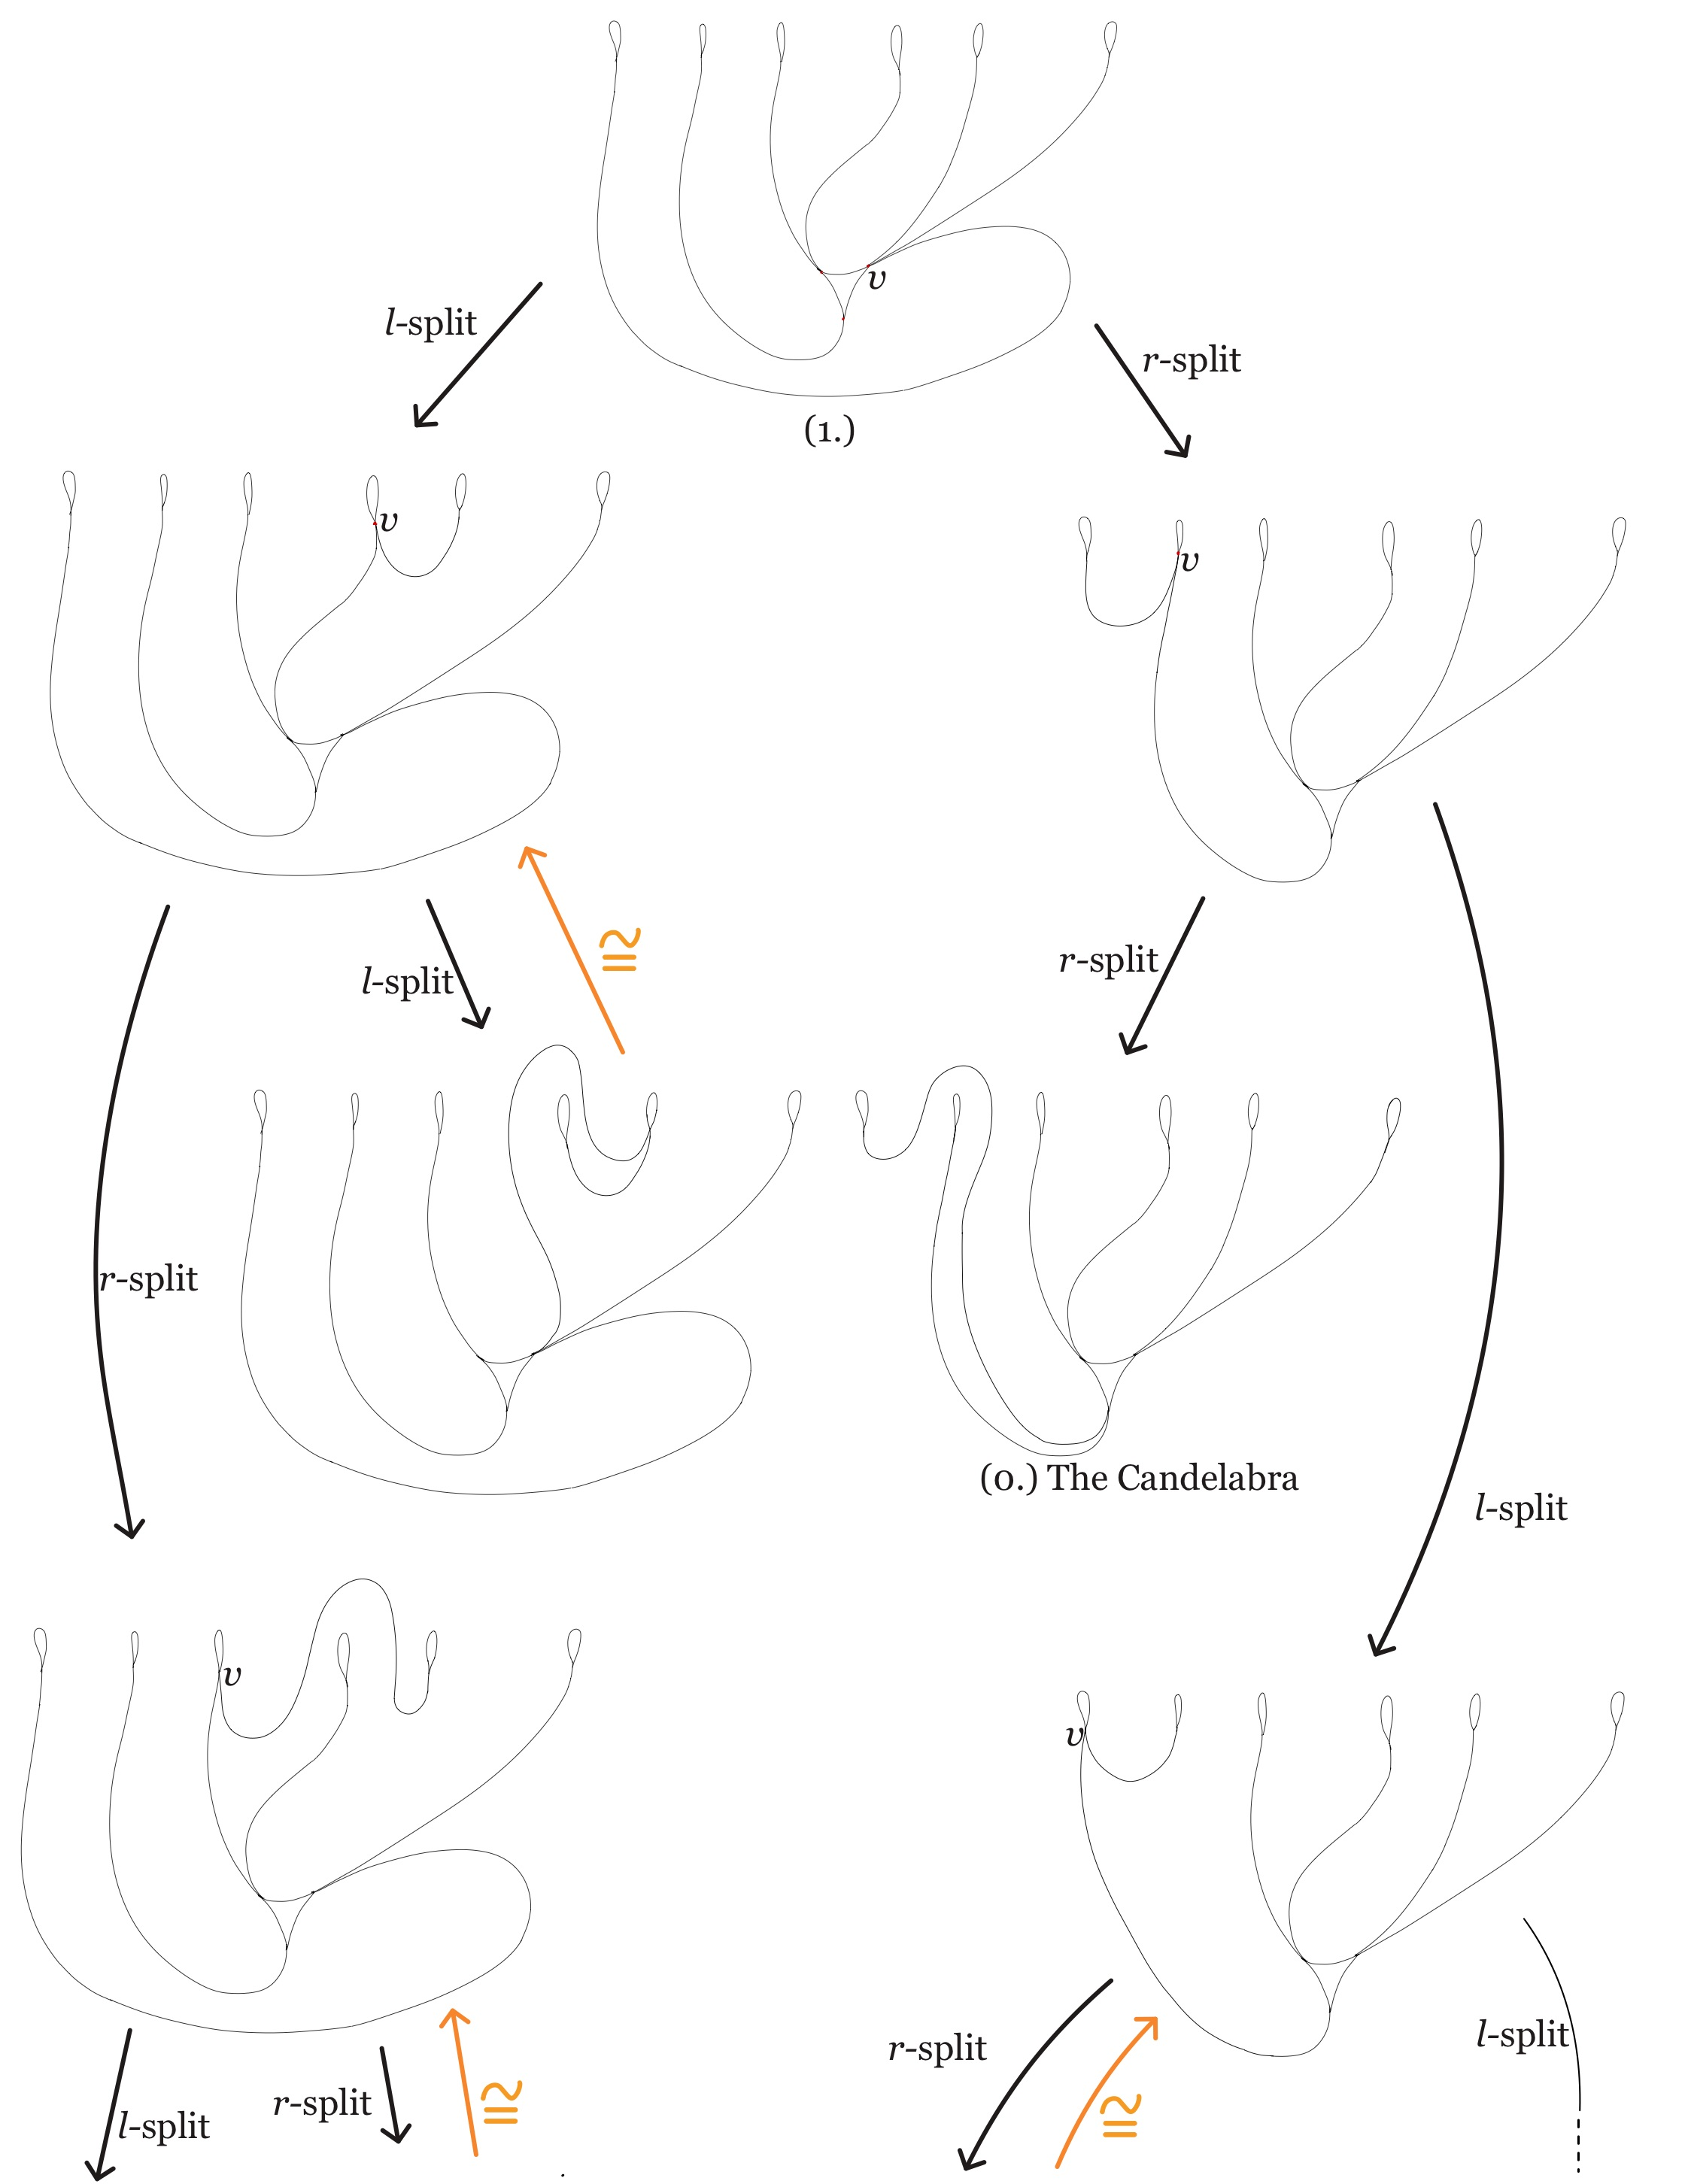
\includegraphics[width=\linewidth, height=0.45\textheight, keepaspectratio]{figures_splitting/Candelabra Splitting-6.jpg}\\[1em]
        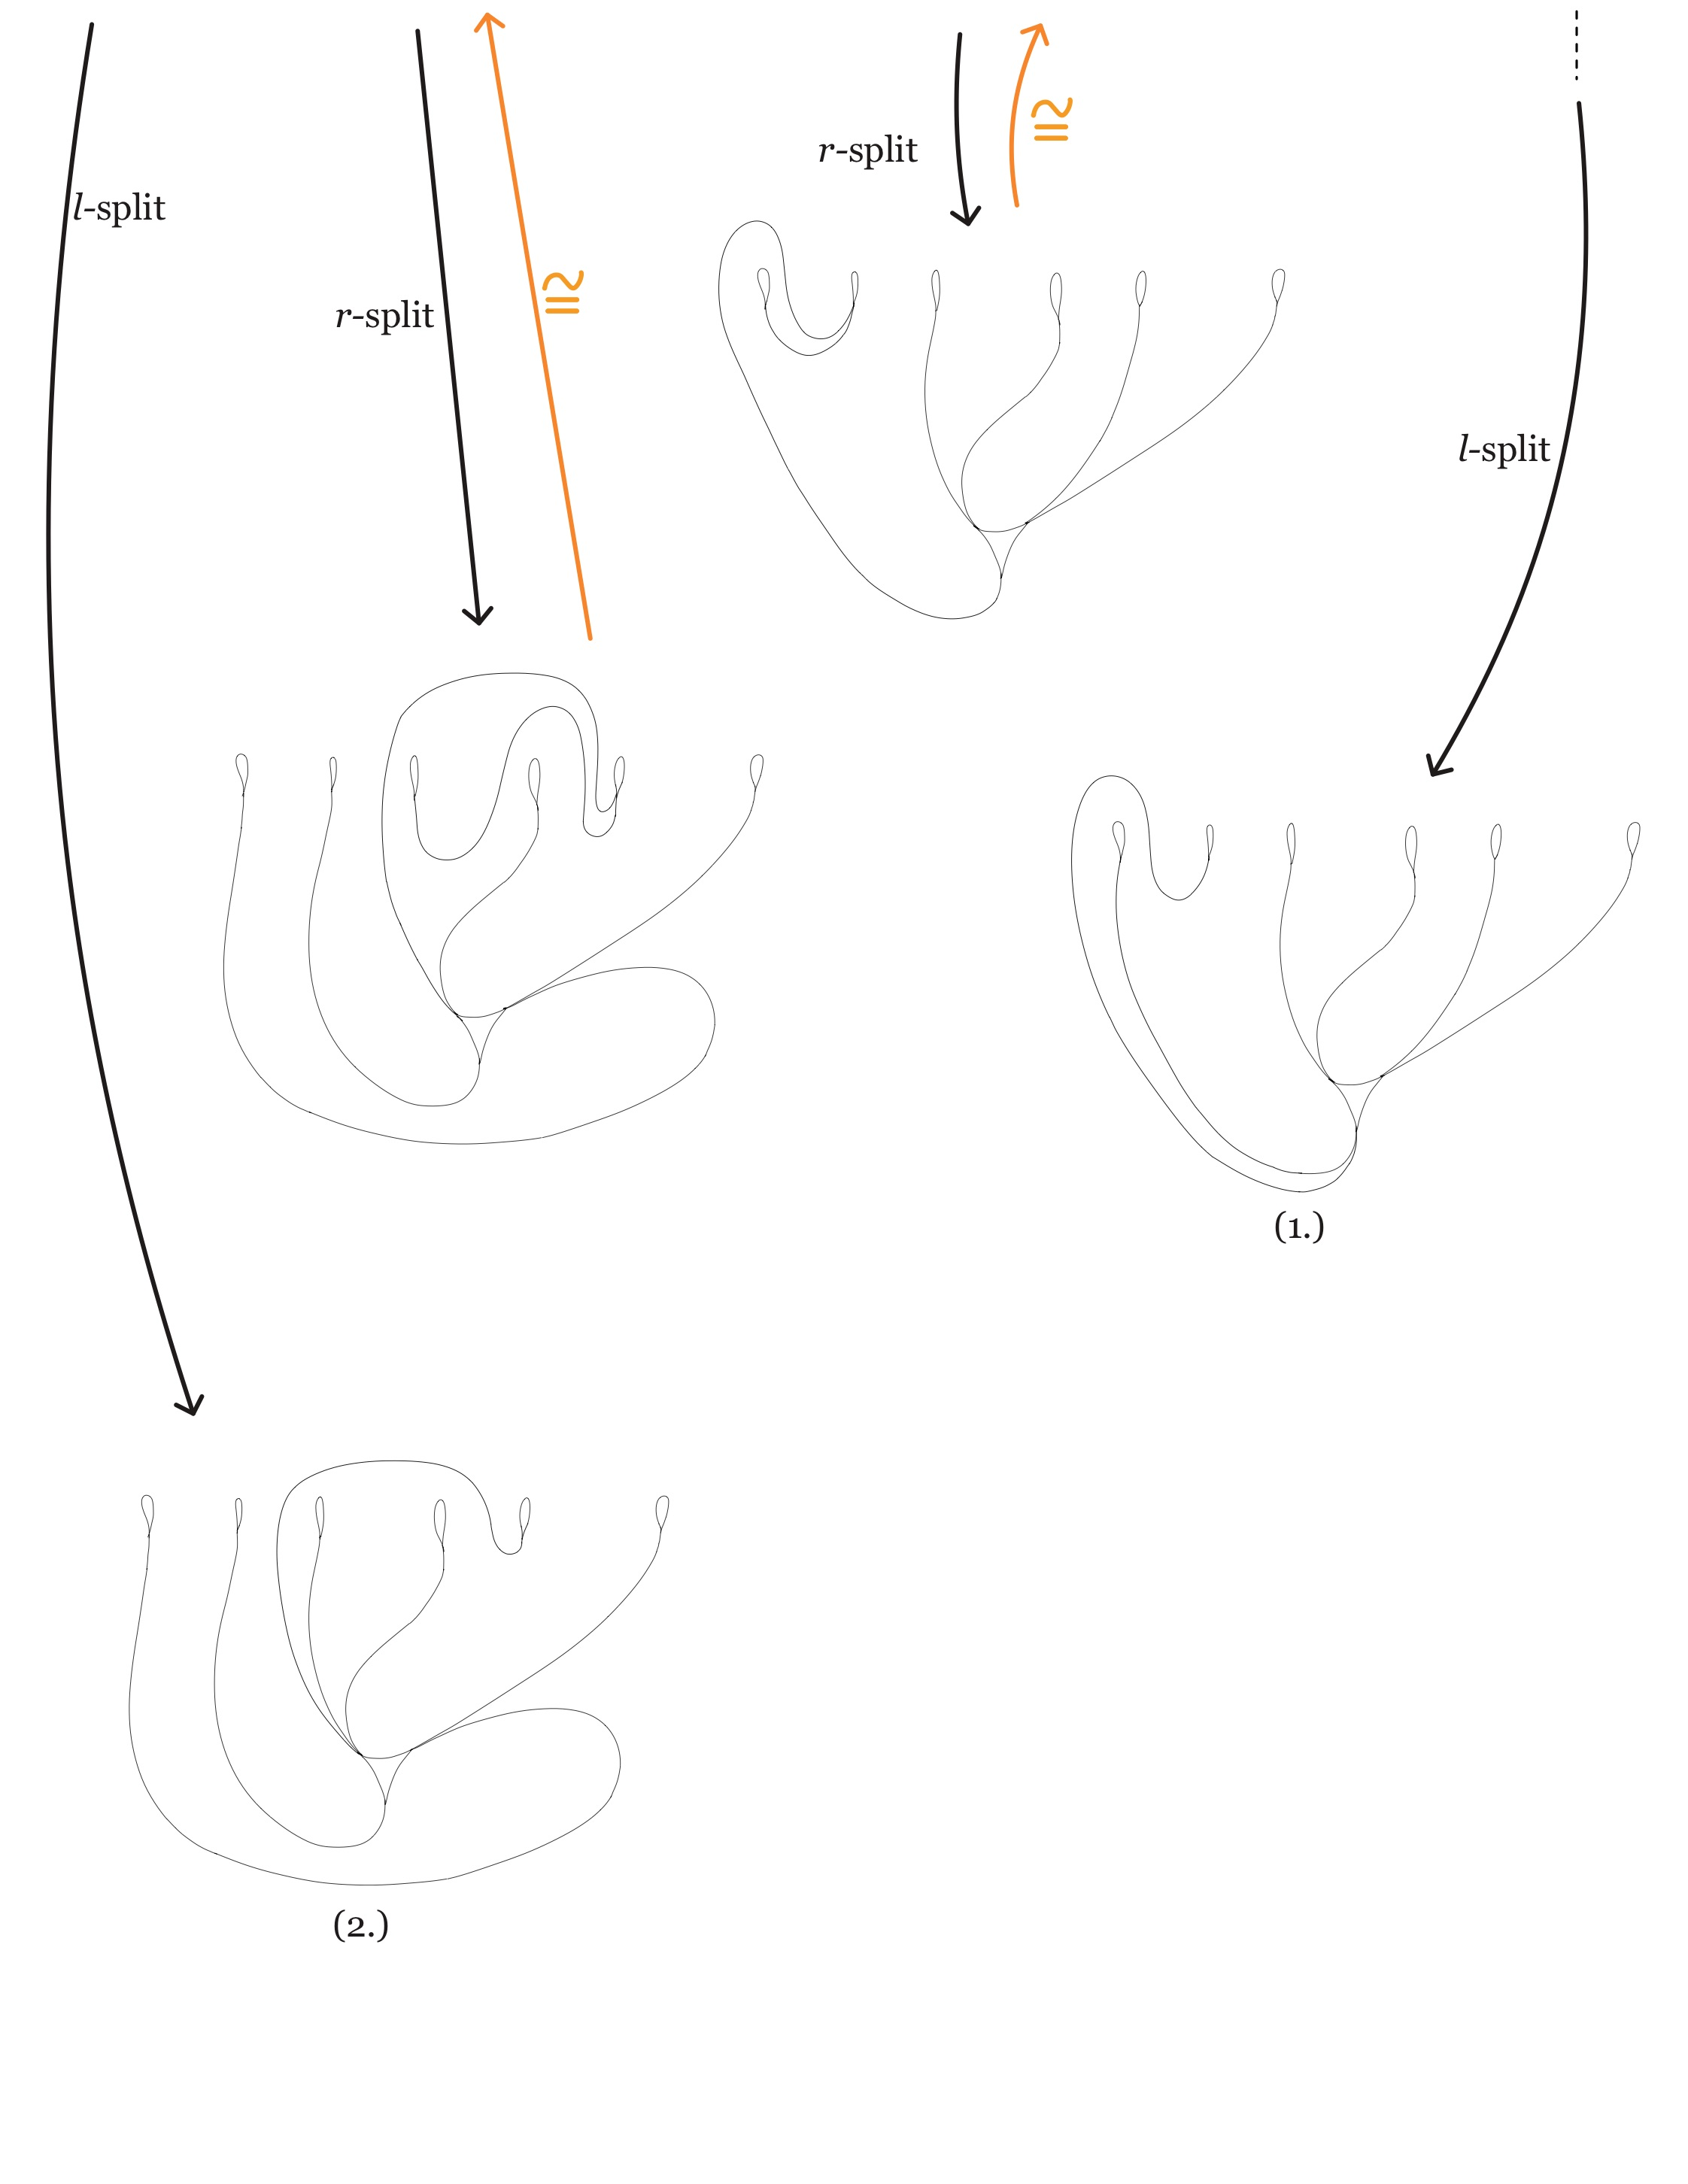
\includegraphics[width=\linewidth, height=0.45\textheight, keepaspectratio]{figures_splitting/Candelabra Splitting-7.jpg}
        \caption{Train Track 1 eventually splits to Train Track 2 or the Candelabra. Mirroring this figure demonstrates that Train Track 2 eventually splits to Train Track 1 or the Candelabra.}
        \label{fig:candelabra_splitting_1}
    \end{figure}

    Observe that Train Tracks 1 and 2 are vertical mirrors of each other. By mirroring the entire splitting sequence of Figure \ref{fig:candelabra_splitting_1}, we obtain a valid splitting sequence for Train Track 2, which necessarily shows that Train Track 2 eventually splits to the Candelabra or back to Train Track 1. By the termination of tight splitting (Theorem \ref{thm:splitting_termination}), this cyclic pattern cannot repeat indefinitely. Therefore, both Train Track 1 and Train Track 2 must eventually split to the Candelabra.

    In conclusion, any pseudo-Anosov map carried by Tracks 1, 2, or 3 is ultimately carried by the Candelabra. Thus, we may assume $\tau$ is strictly the Candelabra train track.
\end{proof}

\begin{figure}[ht]
    \centering
    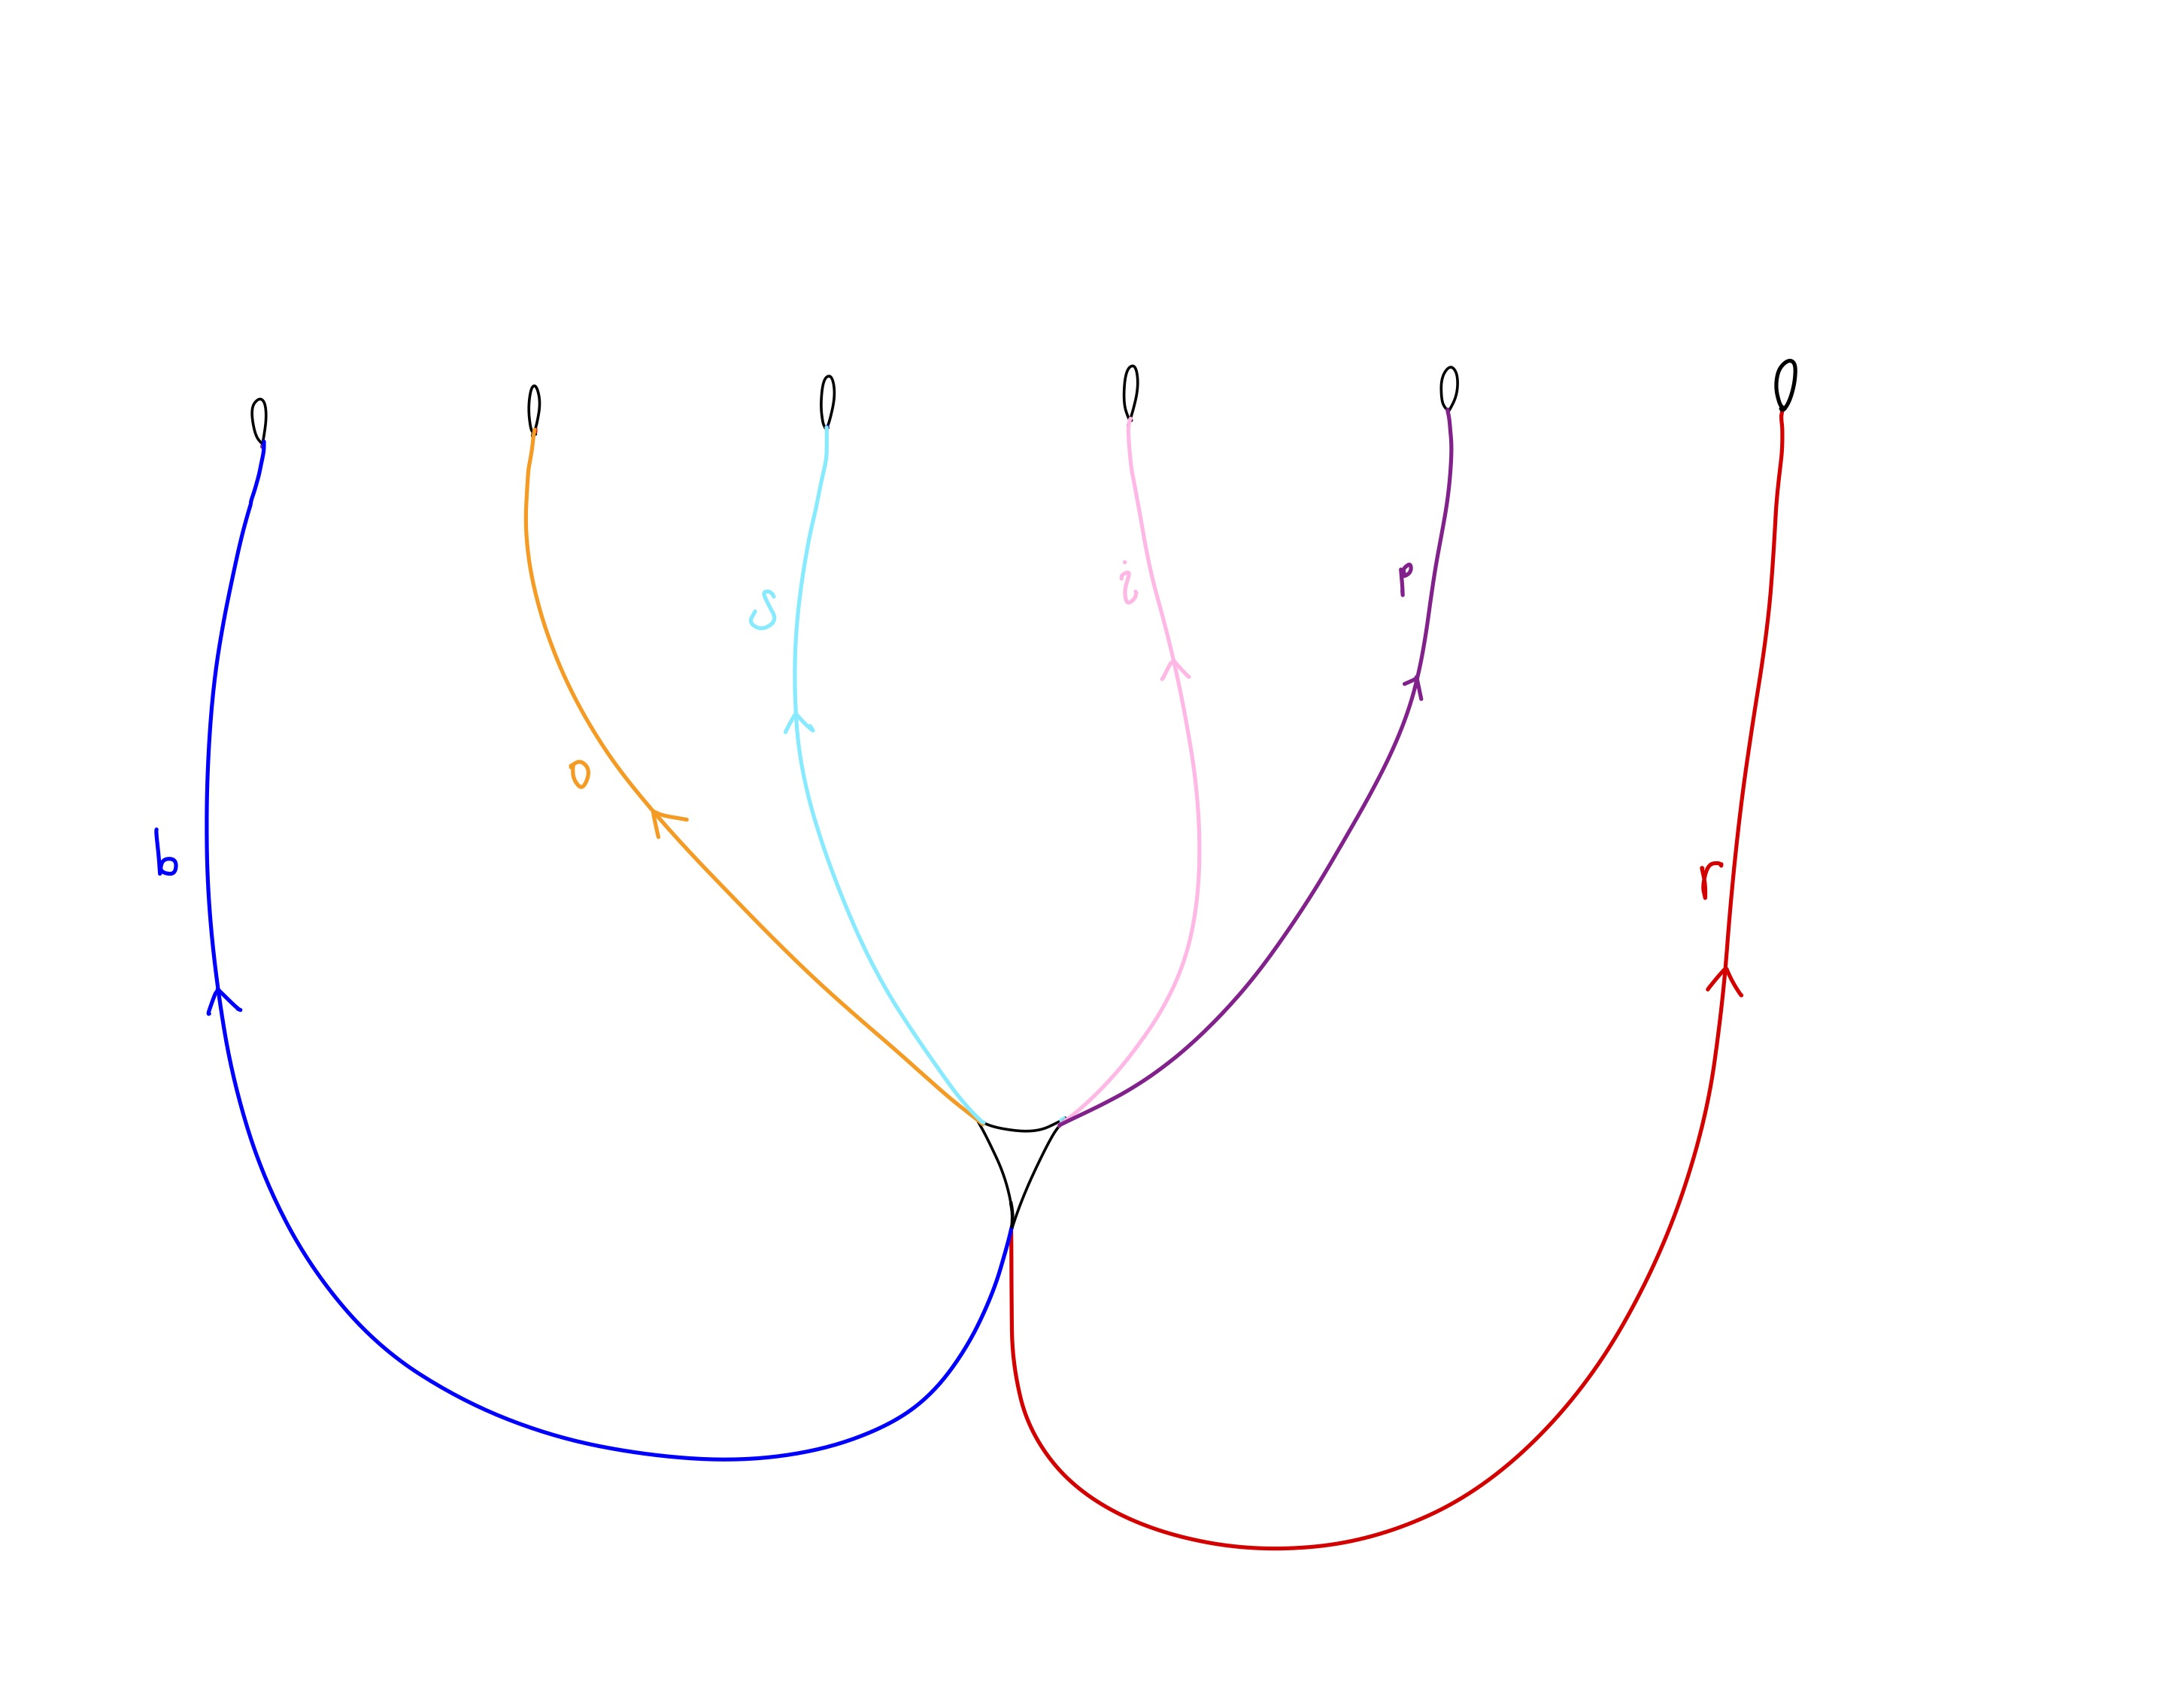
\includegraphics[width=0.8\linewidth]{figures/The Candelabra-1.jpg}
    \caption{The Candelabra train track.}
    \label{fig:candelabra}
\end{figure}

\subsection{Enumeration of Train Track Maps and Braids}

Having reduced our geometric search space to the Candelabra, we execute the case analysis procedure of Section \ref{subsec:case_analysis_procedure}. With no central edge $d$ in this stratum, Cases B, C, D and Assumption A do not arise; the dominant obstruction is Corollary \ref{cor:trace_jointless} (the no-self-occurrence rule for jointless-monogon edges), with the Absorption Obstruction handling most remaining geometric routing decisions. The complete derivation of the surviving maps and their corresponding braid words is presented in Appendix \ref{app:candidate_braids_candelabra}, yielding the following proposition:

\begin{prop}\label{prop:candelabra_34_braids}
    Let $\Phi \colon \Sigma_2^2 \to \Sigma_2^2$ be a pseudo-Anosov mapping class corresponding to the stratum $(3;1^6;3)$ on the disk. If the pseudo-Anosov representative $\phi_\Phi$ has no interior fixed points, then $\Phi$ is conjugate to the lift of one of the 34 braid families explicitly enumerated in Appendix \ref{app:candidate_braids_candelabra}.
\end{prop}

\subsection{Proof of the Main Elimination Theorem}

We are now equipped to definitively prove Theorem \ref{thm:candelabra_stratum_classification}.

\begin{proof}[Proof of Theorem \ref{thm:candelabra_stratum_classification}]
    Suppose, for the sake of contradiction, that the geometric braid representative $\beta$ associated with the knot $K$ belongs to the stratum $(3;1^6;3)$. Since the knot complement is hyperbolic, $\beta$ lifts to a pseudo-Anosov map on $\Sigma_2^2$ that must be fixed-point-free in its interior.

    By Lemma \ref{lem:candelabra_reduction}, up to conjugation and mirroring, $\beta$ must be carried by the Candelabra train track. By Proposition \ref{prop:candelabra_34_braids}, the topological restriction that its lift is fixed-point-free further forces $\beta$ to belong to one of the 34 specific braid families enumerated in Appendix \ref{app:candidate_braids_candelabra}.

    To determine if any of these 34 braid families can correspond to the monodromy of $K$, we apply the homological filters detailed in Section \ref{sec:homological_filtering}. For each of the 34 families, we computationally extract the reduced homological action matrix $A_{\text{red}}$. We test each matrix against the zero-surgery condition (requiring $|\det(I - A_{\text{red}})| = 1$ to ensure the ambient manifold is $S^3$) and the Alexander polynomial condition (requiring $\det(tI - A_{\text{red}}) = (t^2-t+1)^2$).

    Our computational verification demonstrates that \textbf{none} of the 34 families simultaneously satisfy both homological requirements. Since the finite, exhaustive list of topological candidates has been entirely eliminated by algebraic obstruction, no such braid $\beta$ can exist. This concludes the proof.
\end{proof}

%%%%%%%%%%%%%%%%%%%%%%%%%%%%%%%%%%%%%%%%%%%%%%%%%%%%%%%%%%%%%%%%%%%%%%%%
% SKELETON: STRATUM (2;1^6;3^2)
%%%%%%%%%%%%%%%%%%%%%%%%%%%%%%%%%%%%%%%%%%%%%%%%%%%%%%%%%%%%%%%%%%%%%%%%

\section{The Stratum \texorpdfstring{$(2;1^6;3^2)$}{(2;1\textasciicircum 6;3\textasciicircum 2)}}
\label{sec:analysis_2_16_32}

We now turn our attention to the second non-orientable stratum. As in the previous section, our objective is to rigorously eliminate all pseudo-Anosov mapping classes within this stratum as candidates for our specific Birman-Hilden correspondence.

We aim to establish the following elimination theorem:

\begin{theorem}\label{thm:two_triangle_stratum_classification}
    Let $K \subset S^3$ be a hyperbolic knot satisfying $\widehat{HFK}(K) \cong \widehat{HFK}(T_{2,3} \# T_{2,3})$, and let
    \[
    (h, \phi_h, \hat{h}, \hat{\phi}_h, b, \phi_b, \beta, \phi_\beta, \Phi, \phi_\Phi)
    \]
    be the associated Birman-Hilden correspondence data induced by the monodromy of $K$. Then the pseudo-Anosov 6-braid $\beta$ on the disk cannot belong to the stratum $(2;1^6;3^2)$.
\end{theorem}

\subsection{Reducing Candidate Train Tracks via Splitting}

Because the geometric complexity of this stratum involves two interior 3-pronged singularities, the initial state space generated by the folding automaton is significantly larger than that of the Candelabra. We rely heavily on tight splitting and symmetries to reduce this to a computable set.

\begin{lemma}\label{lem:two_triangle_reduction}
    Let $\beta$ be a pseudo-Anosov 6-braid in the stratum $(2;1^6;3^2)$ that lifts to a fixed-point-free mapping class on $\Sigma_2^2$. If $\beta$ is carried by a standard train track $\tau$, then up to conjugation and mirroring, $\tau$ is one of exactly six specific standard train tracks (Tracks 0, 1, 8, 12, 13, and 17).
\end{lemma}

\begin{proof}
    Running the \texttt{autofolder} algorithm on the stratum $(2;1^6;3^2)$ outputs a folding automaton structured as a directed graph with 110 vertices and 412 directed edges. This corresponds to 110 standard train track isomorphism classes. By Corollary \ref{cor:jointless_track}, we may strictly restrict our analysis to the jointless train tracks within this automaton. There are exactly 20 such jointless tracks, depicted in Figure \ref{fig:big_stratum_jointless}.

    \begin{figure*}[p]
        \centering
        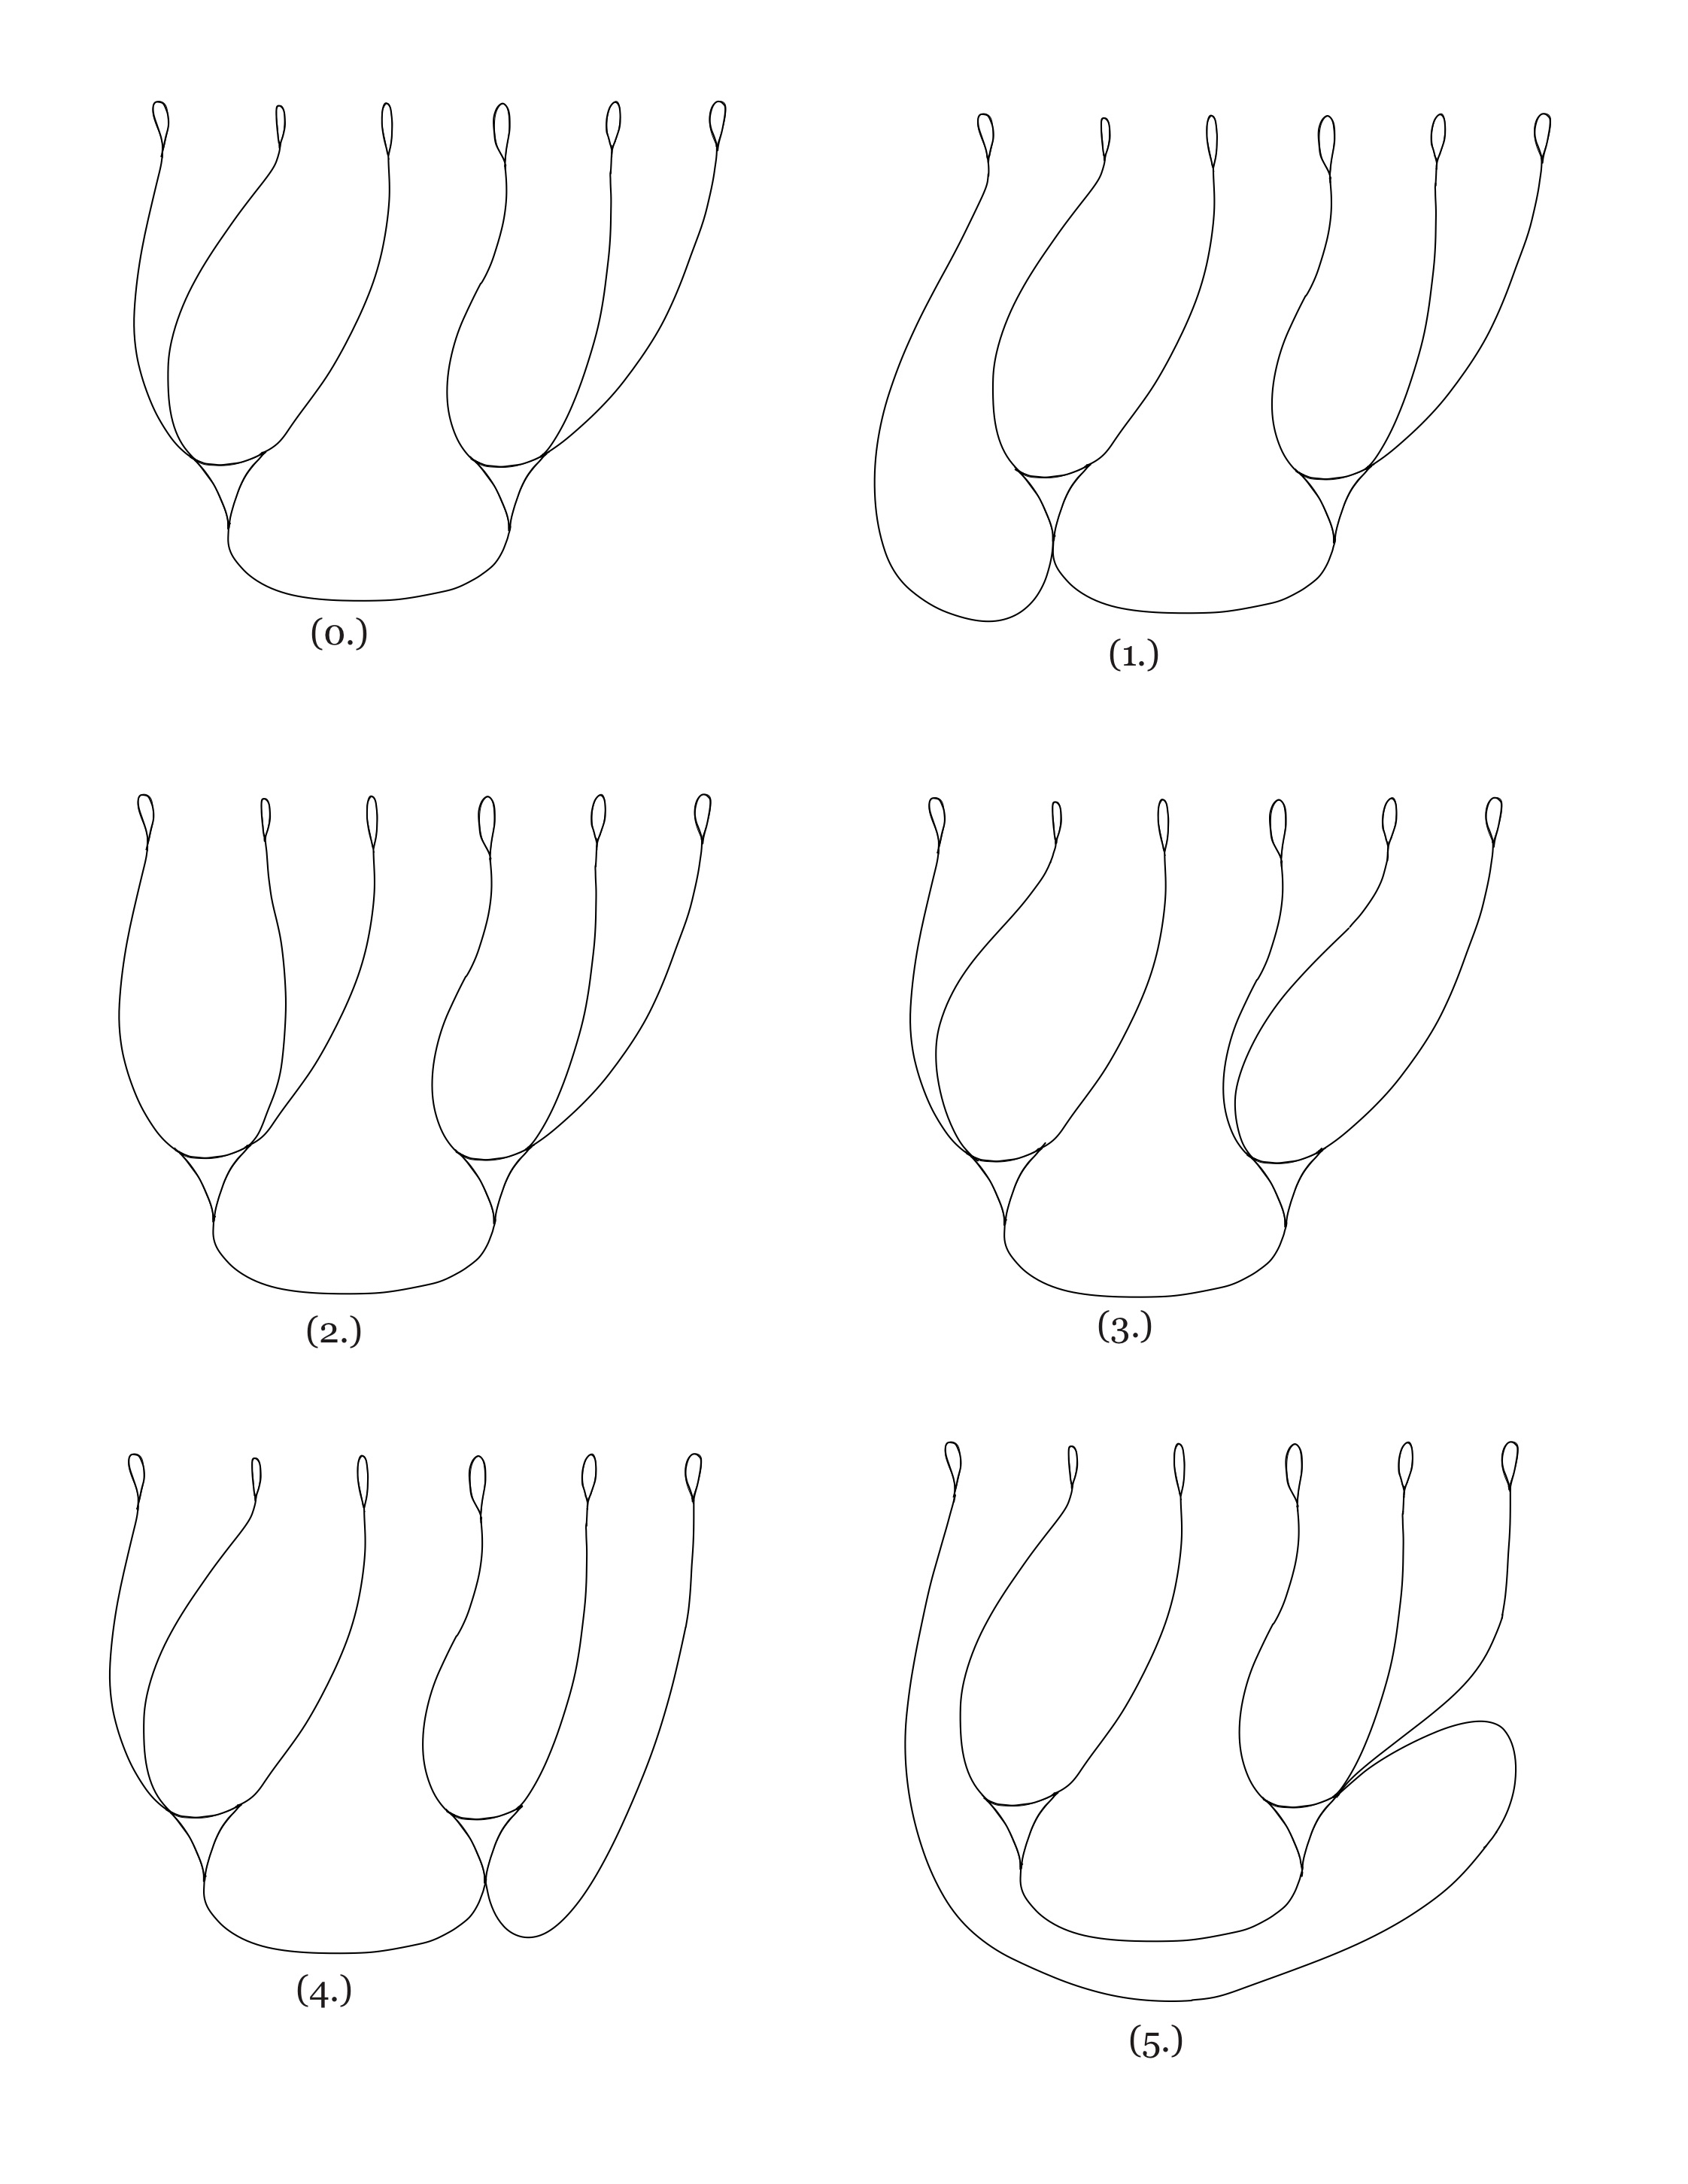
\includegraphics[width=\linewidth, height=0.45\textheight, keepaspectratio]{figures/Big Stratum-1.jpg}\\
        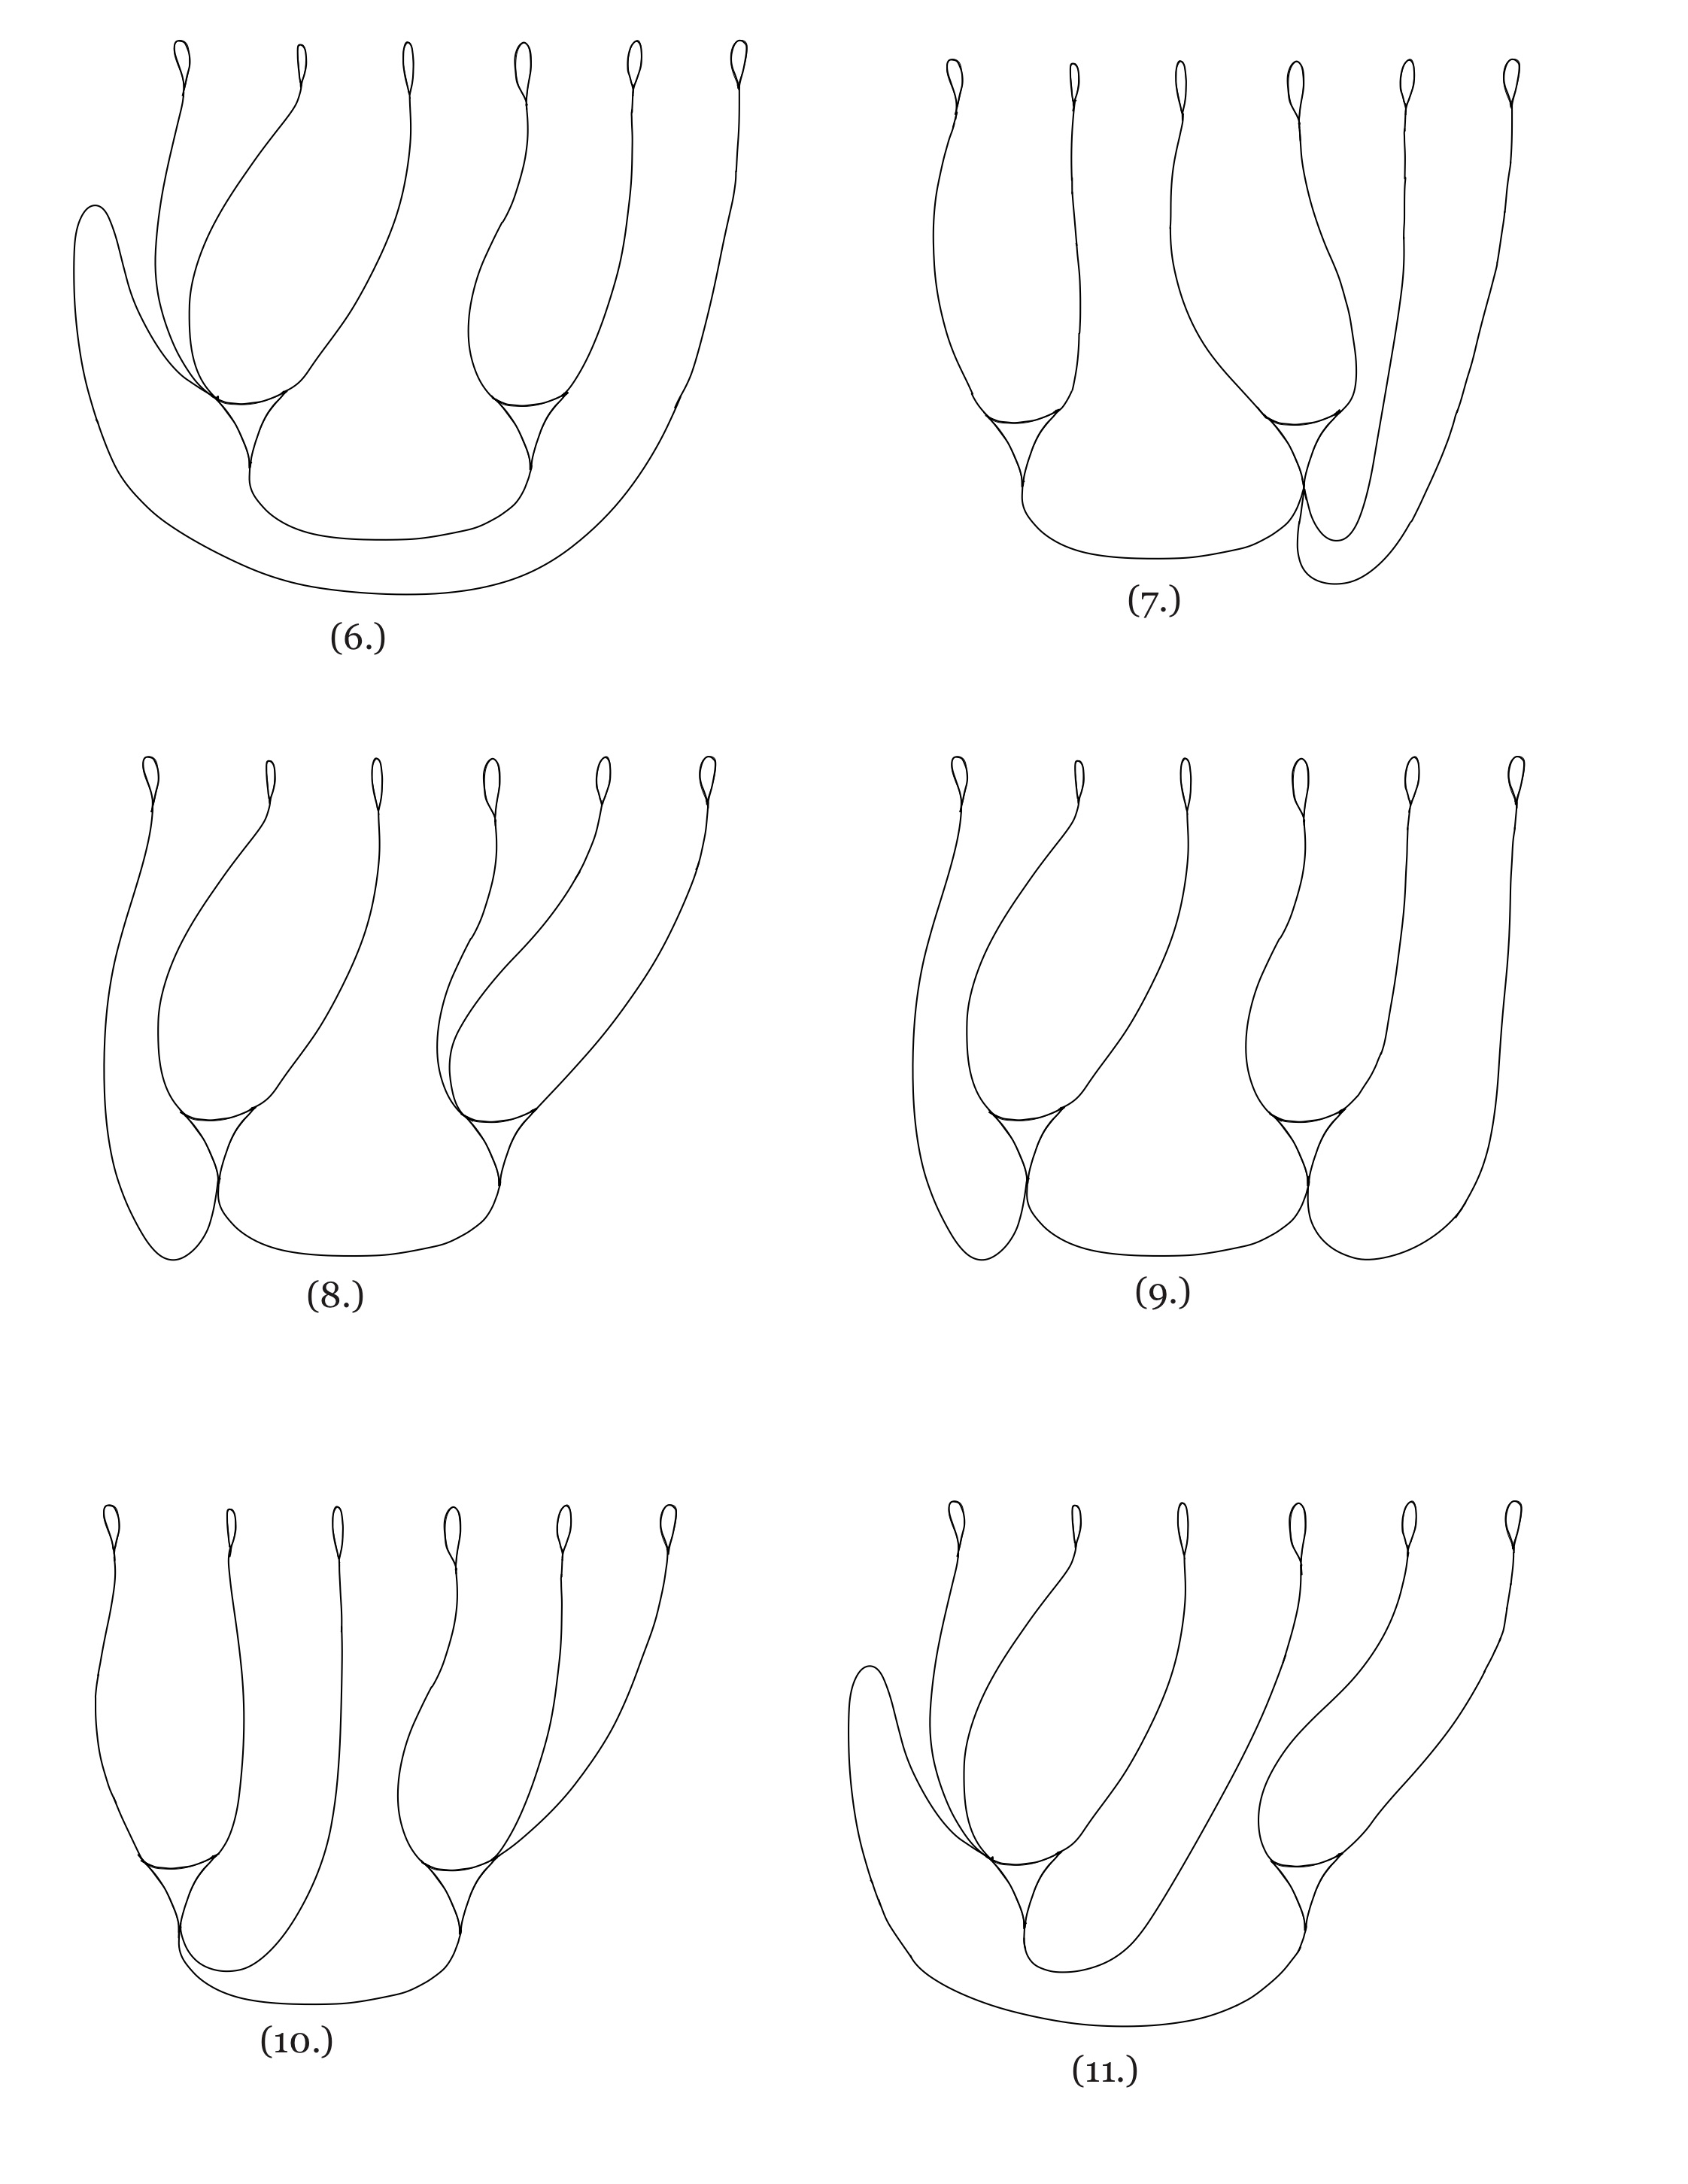
\includegraphics[width=\linewidth, height=0.45\textheight, keepaspectratio]{figures/Big Stratum-2.jpg}
        \caption{The 20 standard jointless train tracks in the stratum $(2;1^6;3^2)$.}
        \label{fig:big_stratum_jointless}
    \end{figure*}

    \begin{figure*}[p]
        \ContinuedFloat
        \centering
        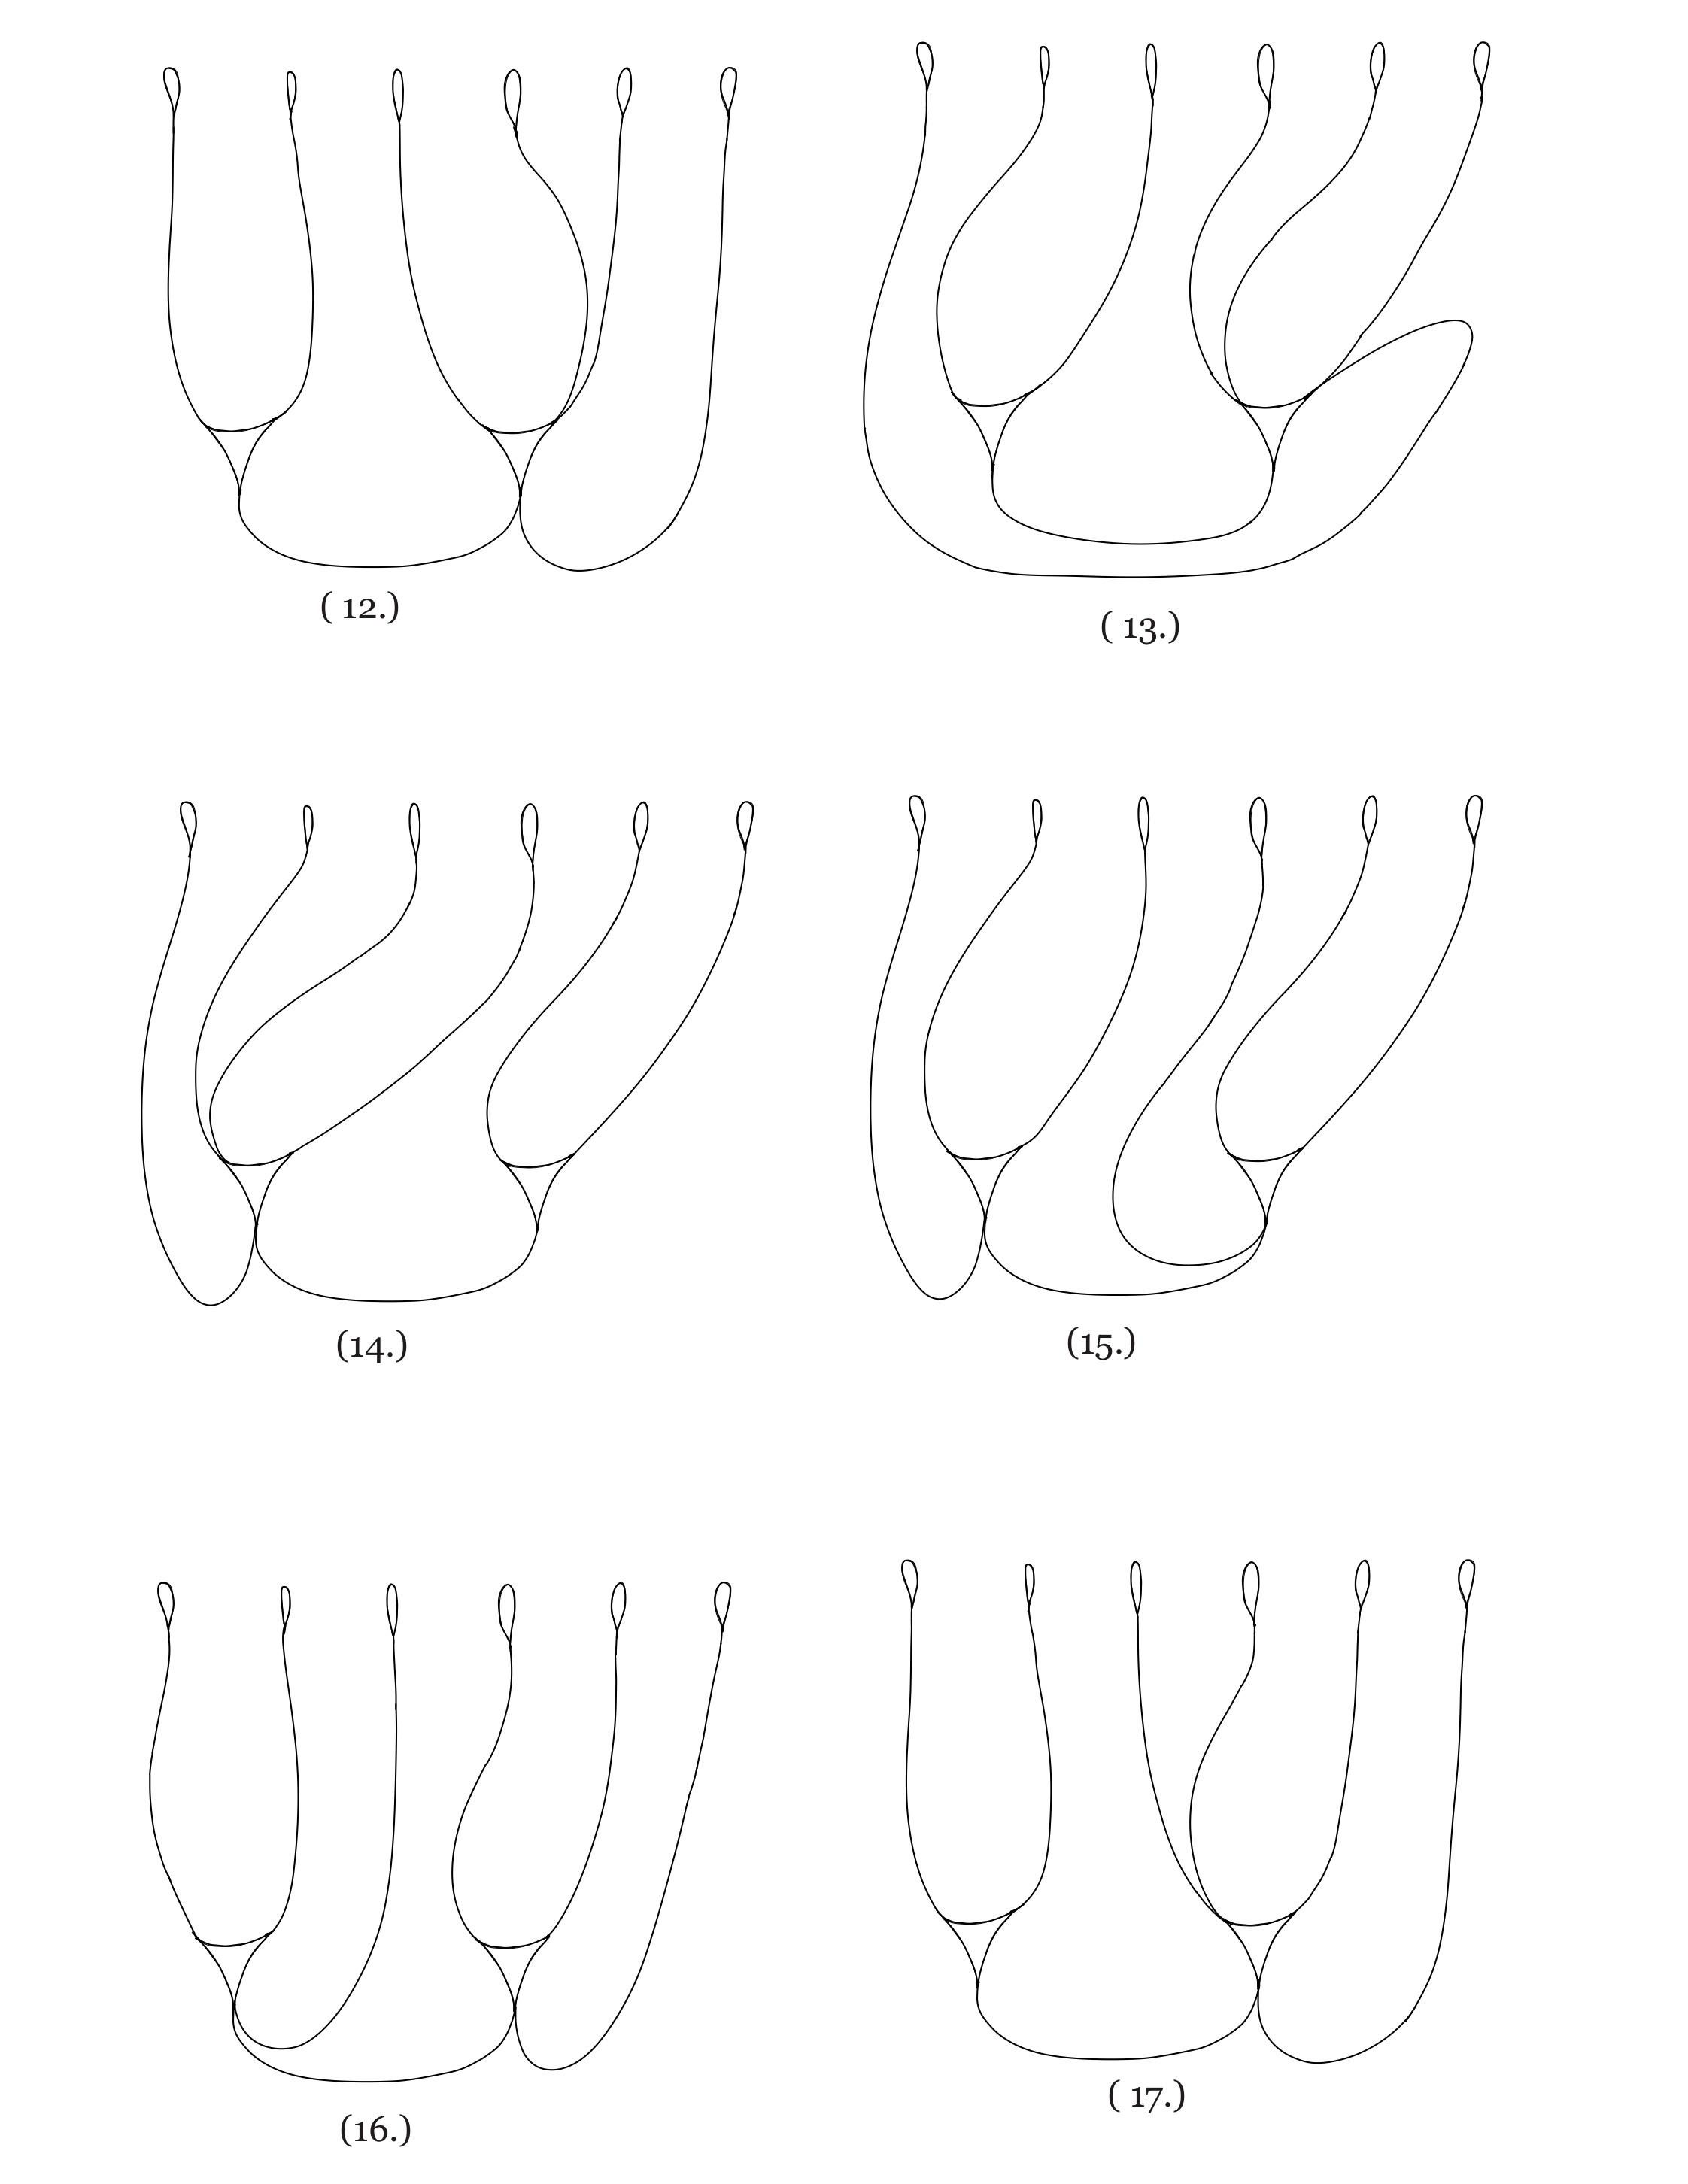
\includegraphics[width=\linewidth, height=0.45\textheight, keepaspectratio]{figures/Big Stratum-3.jpg}\\
        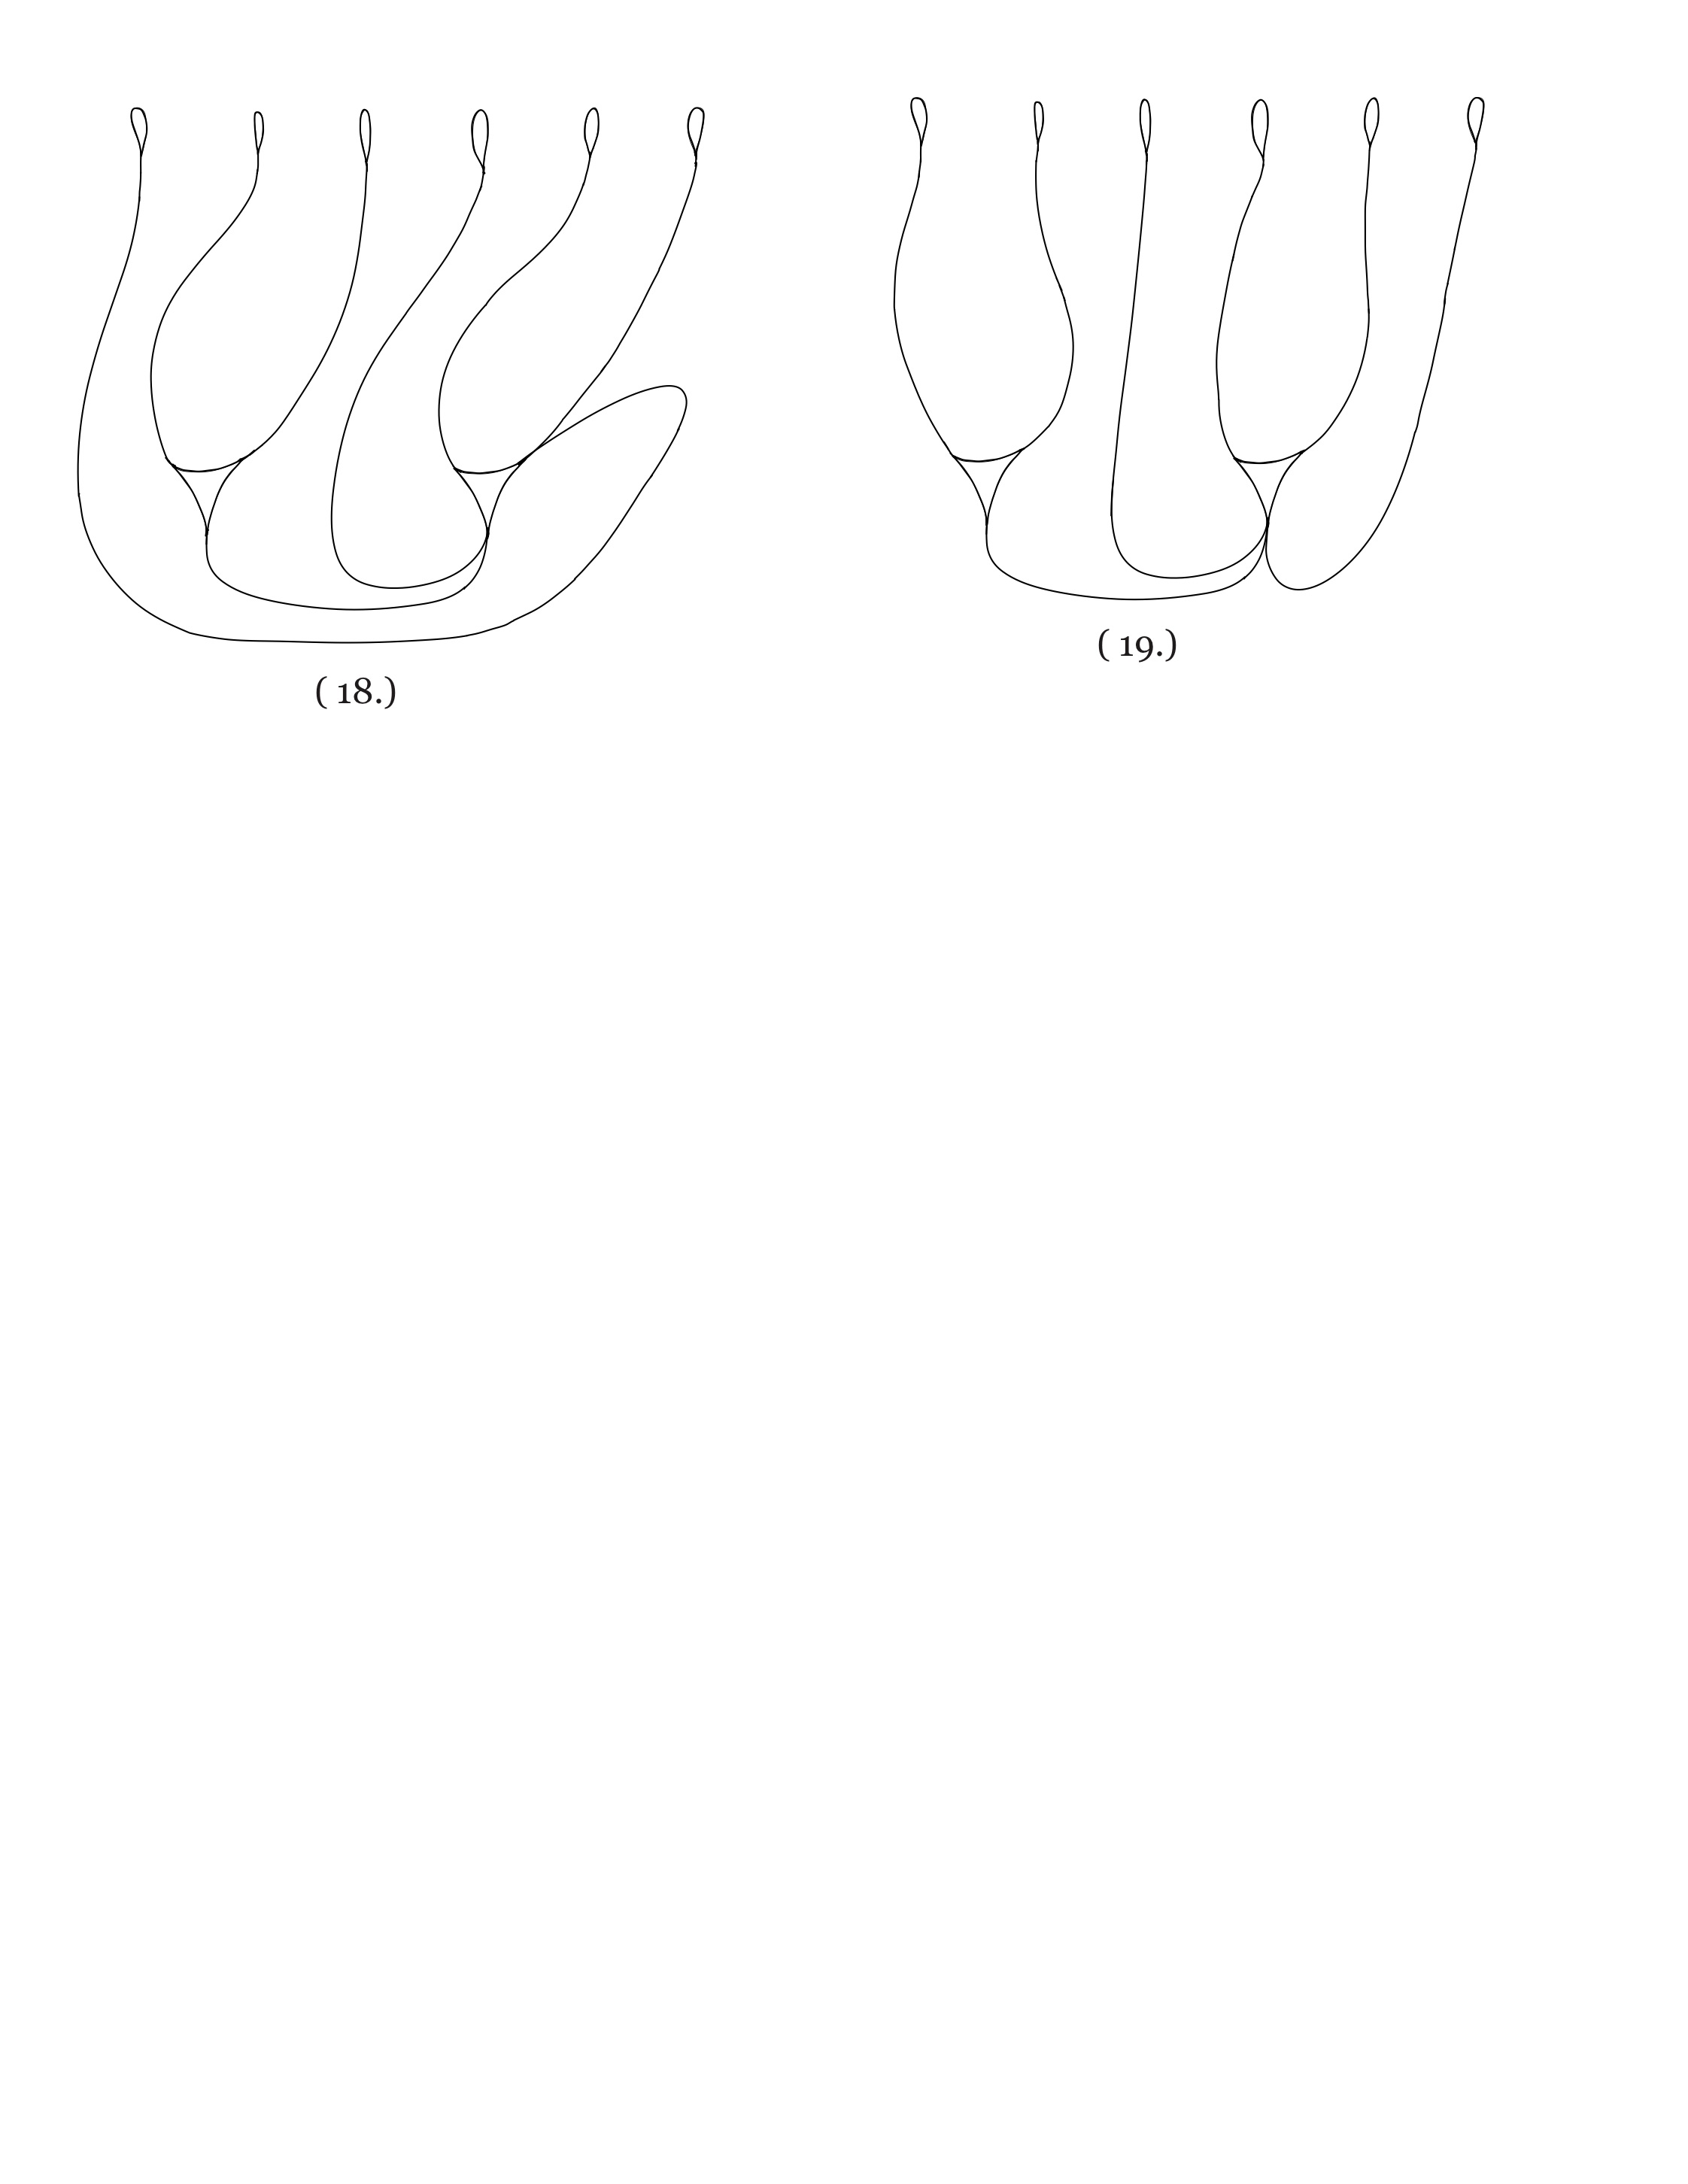
\includegraphics[width=\linewidth, height=0.45\textheight, keepaspectratio]{figures/Big Stratum-4.jpg}
        \caption[]{The 20 standard jointless train tracks in the stratum $(2;1^6;3^2)$ (continued).}
    \end{figure*}

    To simplify the analysis, we identify pairs of train tracks that are vertical mirror images of one another. Any pseudo-Anosov braid carried by a given track can simply be mirrored to be carried by its partner. Among the 20 jointless tracks, we identify the following mirror pairs:
    \begin{itemize}
        \item (1) and (4)
        \item (2) and (3)
        \item (5) and (6)
        \item (7) and (11)
        \item (8) and (10)
        \item (12) and (14)
        \item (15) and (16)
        \item (17) and (18)
    \end{itemize}
    By selecting one representative from each pair, we reduce the space to 12 base tracks: (0), (1), (2), (5), (7), (8), (9), (12), (13), (15), (17), and (19).

    Finally, we deploy the tight splitting operation. Because each train track possesses two infinitesimal triangles ($3$-gons), an initial tight splitting can occur at either of the two corresponding loop switches. We compute the exhaustive splitting sequences for these 12 base tracks, the complete diagrams for which are provided in Appendix \ref{app:splitting_big_stratum}.

    As demonstrated in the appendix, the splitting sequences for tracks (19), (17), (15), (13), (12), (9), (8), (7), (5), (2), and (1) recursively terminate by splitting into one of the following six base tracks: (0), (1), (8), (12), (13), and (17). Therefore, up to conjugation and mirroring, any pseudo-Anosov map in this stratum must be carried by one of these final six tracks, shown in Figure \ref{fig:final_six_tracks}.
\end{proof}

\begin{figure}[ht]
    \centering
    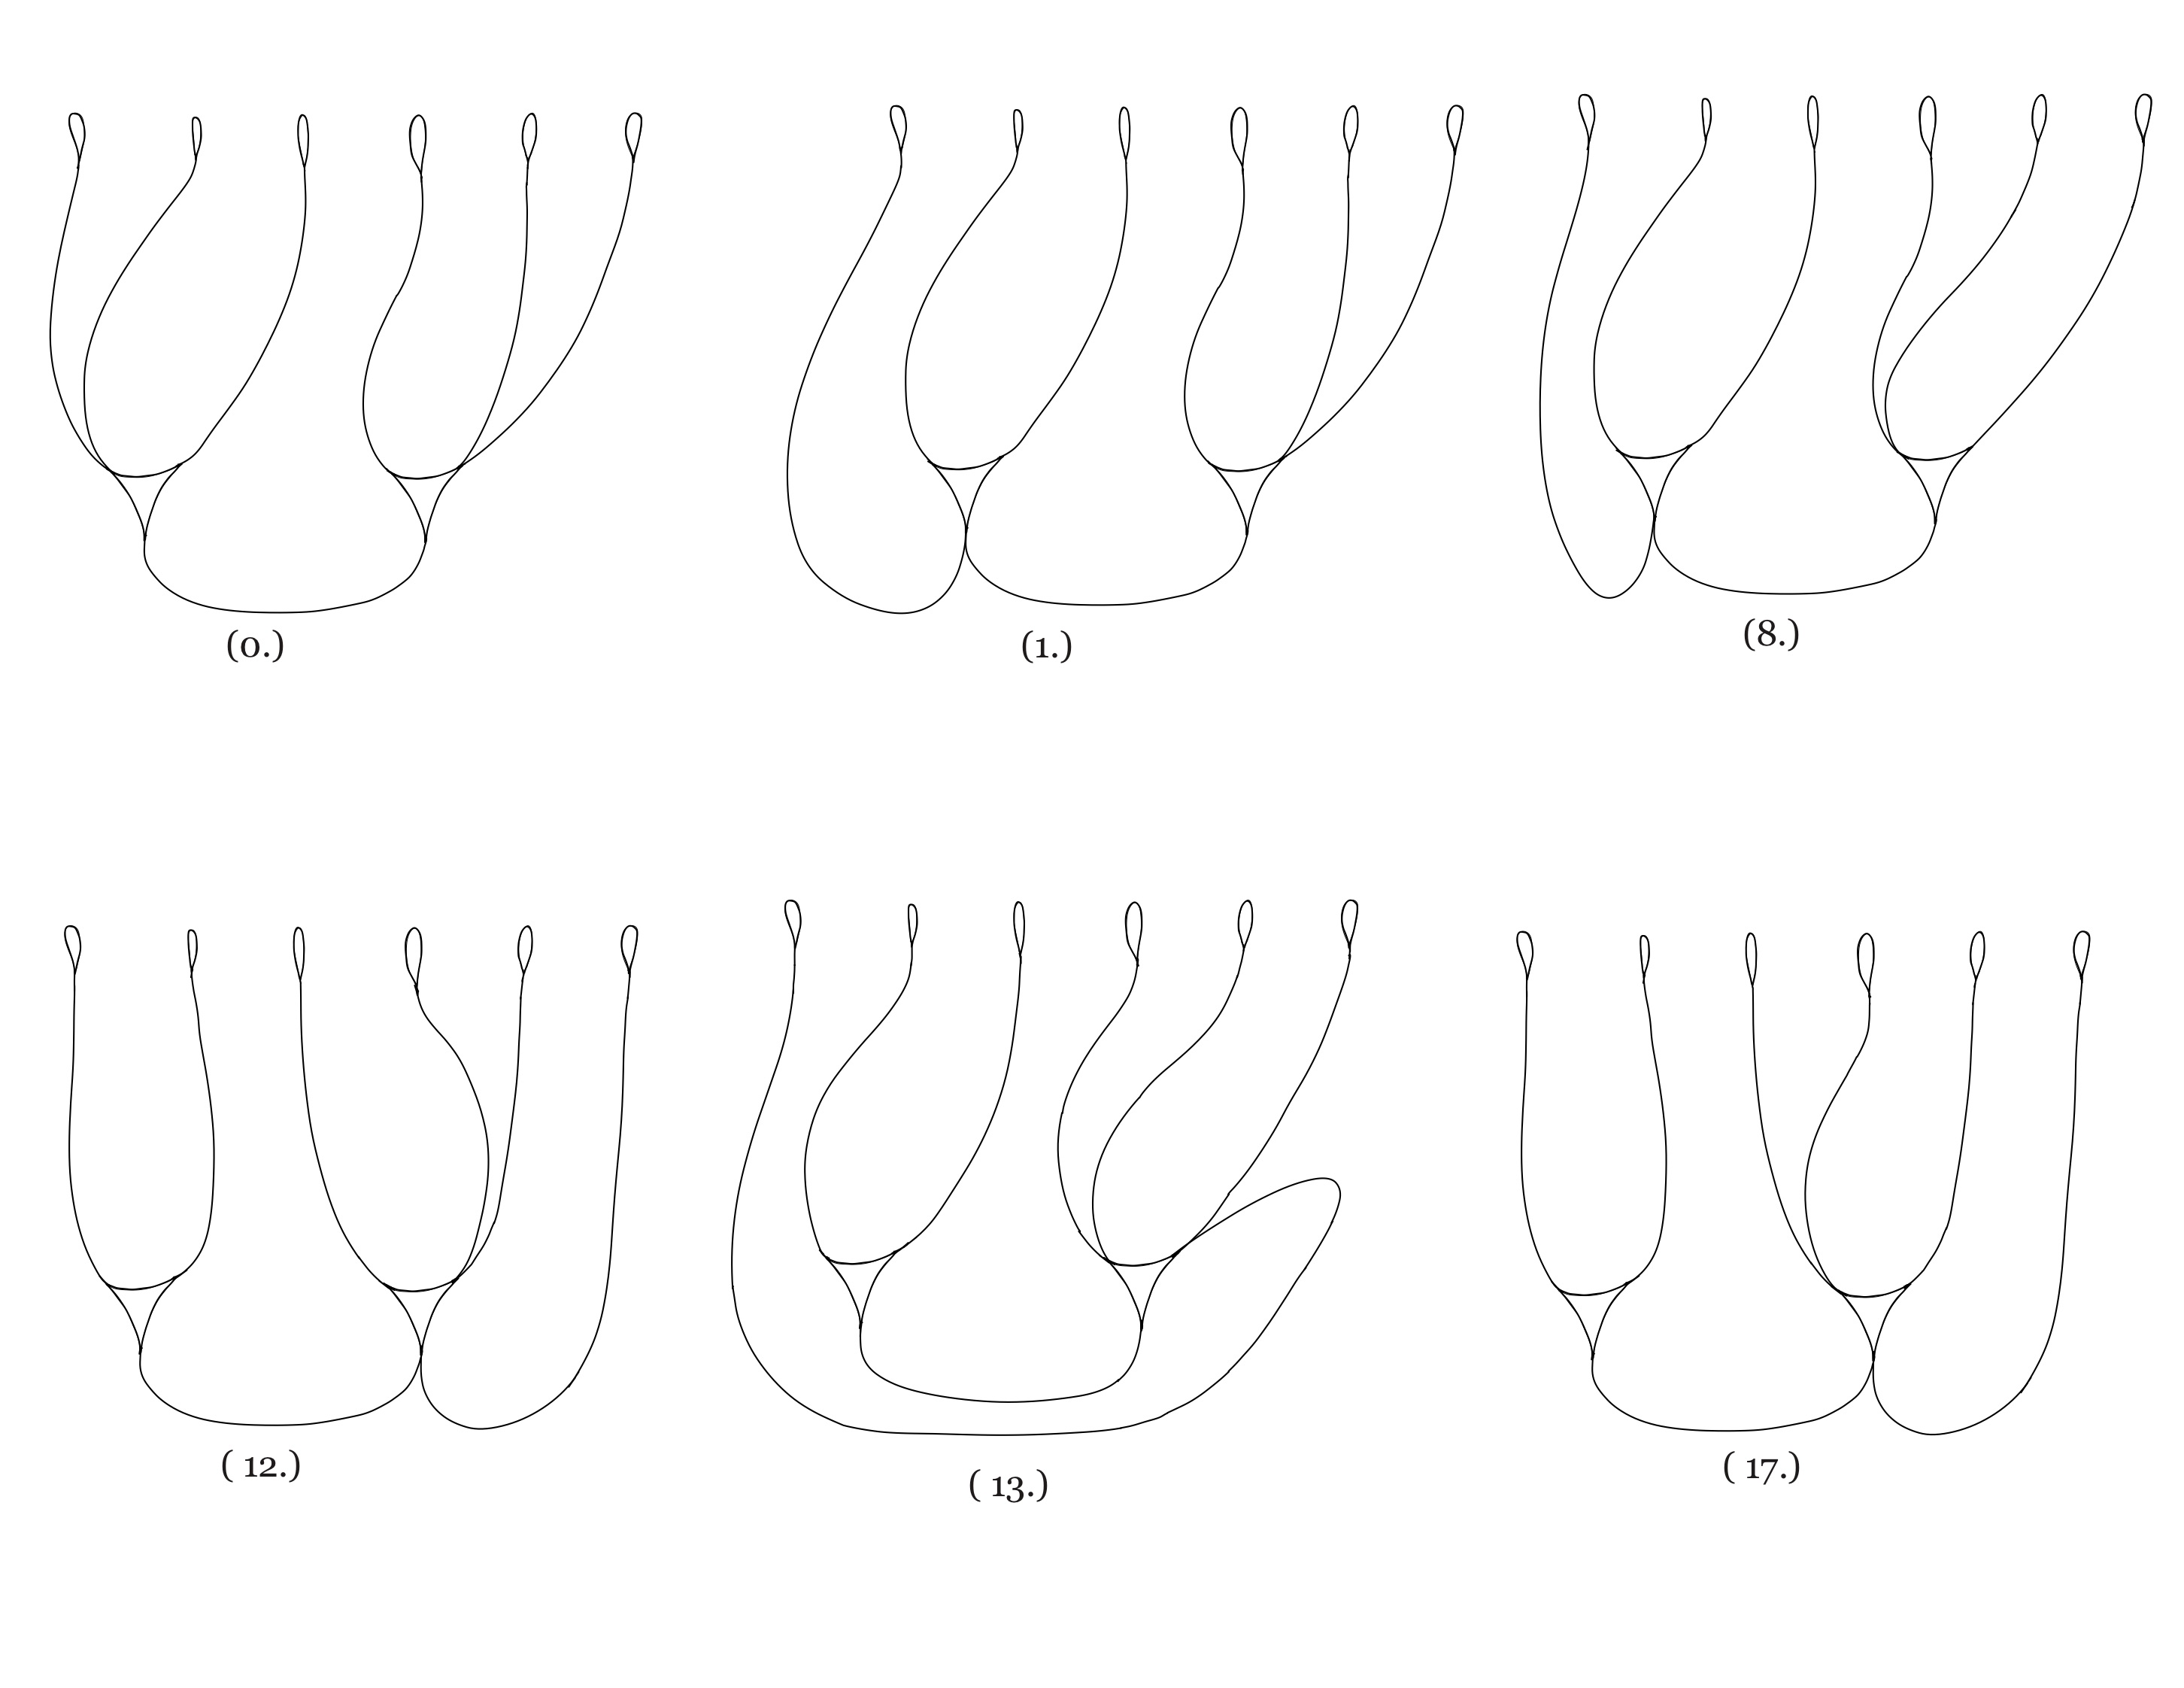
\includegraphics[width=\linewidth]{figures/Six Tracks-1.jpg}
    \caption{The six irreducible standard train tracks for the stratum $(2;1^6;3^2)$. Up to equivalence, all valid maps must be carried by one of these tracks.}
    \label{fig:final_six_tracks}
\end{figure}

\subsection{Enumeration of Train Track Maps and Braids}
With the geometric state space reduced to six invariant tracks, we execute the case analysis procedure of Section \ref{subsec:case_analysis_procedure} on each. The parity constraints on $f_\beta(d)$ and $f_\beta(\bar{d})$ (the Trace Lemma applied to the central edge in its four-case form) become the decisive obstruction in this stratum: Situation $\alpha$ produces the bulk of non-termination eliminations (the dotted lines circle the outer perimeter without joining), and Situation $\beta$ produces the bulk of direct-violation eliminations (the dotted lines are trapped in a pocket forcing an odd-parity return). Path mills arise as a secondary non-termination obstruction for the non-dotted edges.

For Track 12, this analysis yields no surviving train track maps: every candidate transition word is excluded either by a tracing violation of Corollary \ref{cor:trace_jointless} or by absorption between adjacent edge images. The full case analysis for Track 12 is included in Appendix \ref{app:case_analysis_track12} for completeness. Consequently, no fixed-point-free pseudo-Anosov braid in the stratum $(2;1^6;3^2)$ is carried by Track 12, and the analysis below treats only the remaining five tracks where surviving candidates exist.

This combinatorial exhaustion yields a finite set of surviving train track map families on the five remaining tracks. The step-by-step derivation and the explicit extraction of their corresponding braid words are detailed in Appendices \ref{app:candidate_braids_track_0}, \ref{app:candidate_braids_track_1}, \ref{app:candidate_braids_track_8}, \ref{app:candidate_braids_track_13}, and \ref{app:candidate_braids_track_17}. This analysis establishes the following proposition:

\begin{prop}\label{prop:two_triangle_braids}
    Let $\Phi \colon \Sigma_2^2 \to \Sigma_2^2$ be a pseudo-Anosov mapping class corresponding to the stratum $(2;1^6;3^2)$ on the disk. If the pseudo-Anosov representative $\phi_\Phi$ has no interior fixed points, then $\Phi$ is conjugate to the lift of one of the finite braid families enumerated for Tracks 0, 1, 8, 13, and 17 (Appendices \ref{app:candidate_braids_track_0}, \ref{app:candidate_braids_track_1}, \ref{app:candidate_braids_track_8}, \ref{app:candidate_braids_track_13}, \ref{app:candidate_braids_track_17}).
\end{prop}

\subsection{Proof of the Main Elimination Theorem}

With our topological candidates isolated, we arrive at the final algebraic obstruction.

\begin{proof}[Proof of Theorem \ref{thm:two_triangle_stratum_classification}]
    Suppose, for the sake of contradiction, that the geometric braid representative $\beta$ associated with the knot $K$ belongs to the stratum $(2;1^6;3^2)$. Because the target knot complement is hyperbolic, $\beta$ lifts to a pseudo-Anosov map on $\Sigma_2^2$ that is fixed-point-free in its interior.

    By Lemma \ref{lem:two_triangle_reduction}, $\beta$ must be carried by one of the six irreducible train tracks. By Proposition \ref{prop:two_triangle_braids}, the Trace Lemma forces $\beta$ to belong to one of the specific braid families enumerated in the corresponding track appendices.

    We route these surviving candidates through the homological filters detailed in Section \ref{sec:homological_filtering}. For each candidate family, we compute the reduced homological action matrix $A_{\text{red}}$. We test these matrices against the zero-surgery requirement ($|\det(I - A_{\text{red}})| = 1$) and the Alexander polynomial requirement ($\det(tI - A_{\text{red}}) = (t^2-t+1)^2$).

    Computation demonstrates that none of the candidate families from these appendices simultaneously satisfy both necessary conditions. Because the finite set of topological candidates has been entirely eliminated, no such braid $\beta$ can correspond to the monodromy of $K$. This completes the proof.
\end{proof}